\documentclass[pdftex,11pt]{book}
\usepackage[pdftex]{graphicx}
\usepackage[activeacute,spanish]{babel}
\usepackage[T1]{fontenc}
\usepackage[protrusion=true,expansion=true]{microtype}
\usepackage{enumitem}
\usepackage{lmodern}
\usepackage[latin1]{inputenc}
\usepackage{geometry}
\geometry{verbose,dvips,paperwidth=5in,paperheight=8in,tmargin=.65in,bmargin=.9in, left=0.80in, right=0.65in}
\usepackage{lettrine}
\usepackage[raggedright]{titlesec}

\newcommand{\degree}{\ensuremath{^\circ}}

\setcounter{secnumdepth}{0} 
\setcounter{tocdepth}{2}

\titleformat{\section}
  {\raggedright\normalfont\scshape}{\thesection}{1em}{}
	
\titleformat{\subsection}
  {\raggedright\normalfont\slshape}{\thesection}{1em}{}	
	
\widowpenalty=10000
\clubpenalty=10000
\brokenpenalty=10000\relax

\setlist[itemize]{leftmargin=*, noitemsep}

\makeatletter
\def\@makechapterhead#1{%
  \vspace*{20\p@}%
  {\parindent \z@ \raggedright
    \Large
    \ifnum \c@secnumdepth >\m@ne
        \textsc{\Large#1}
        \par\nobreak    
    \fi
    \interlinepenalty\@M
    \vskip 110\p@
  }}
  
  \def\notesname{}%


\def\@makeschapterhead#1{%
  \vspace*{20\p@}%
  {\parindent \z@ \raggedright
    \Large
    \ifnum \c@secnumdepth >\m@ne
        \textsc{\Large#1}
        \par\nobreak    
    \fi
    \interlinepenalty\@M
    \vskip 110\p@
  }}
  
  \def\notesname{}%

\makeatletter

\usepackage{fancyhdr}
\fancyhead[LE,RO]{}
\fancyhead[CE,CO]{}
\fancyhead[RE,LO]{}
\fancyfoot[LO,RE]{}
\fancyfoot[CE,CO]{}
\fancyfoot[LE,RO]{\thepage}

\usepackage{hyperref}

\begin{document}

\renewcommand{\headrulewidth}{0pt}

\normalsize

\newpage
\thispagestyle{empty}
\mbox{}

\newpage
\thispagestyle{empty}
\mbox{}

\begin{frontmatter}
\pagestyle{empty}

\vspace*{3cm}
\begin{center}
\Large{\emph{Introducci?n a los Sistemas de Informaci?n Geogr?fica}}
\end{center}
\newpage

\null
\vfill
\scriptsize
\noindent
Introducci?n a los Sistemas de Informaci?n Geogr?fica\\
Copyright \copyright 2016 V?ctor Olaya\\

\vspace{10mm}
\noindent Versi?n revisada el \today{}\\

\vspace{6mm}
\noindent
Permission is granted to copy, distribute or modify this work under the terms of the Creative Commons, which can be found at \url{www.creativecommons.org}.
The license applies to the entire text, including the images created by the author.
All images are by the author unless explicitly stated.
This book can be downloaded and consulted freely in various formats, including editable formats from \url{http://victorolaya.com}.\\

\noindent
The names of products or corporations that appear in the text may constitute trademarks and must only used for identification.
% Unsure
Also, the mention or absence of such products does not express any recommendation on the part of the author.\\

\vspace{5mm}
\noindent \rule{\textwidth}{1pt}

\newpage

\makeatletter
\newlength\drop
\newcommand*{\titleGM}{%
\thispagestyle{empty}
\begingroup% Gentle Madness
\drop = 0.1\textheight
\vspace*{\baselineskip}
\vfill
\hbox{%
\hspace*{0.1\textwidth}%
\rule{1pt}{\dimexpr\textheight-28pt\relax}%
\hspace*{0.05\textwidth}% 
\parbox[b]{0.75\textwidth}{%
\vbox{%
    \vspace{\drop}
    {\Large\textsc{V?ctor Olaya}\par}\vskip3.5\baselineskip
    {\Huge\bfseries\raggedright{Introducci?n a los Sistemas de Informaci?n Geogr?fica}\par}
    \vspace{2.5cm}
    \vspace{0.4\textheight}
}% end of vbox
}% end of parbox
}% end of hbox
\vfill
\null
\endgroup}
\makeatother
\titleGM

\cleardoublepage
\normalsize

\chapter*{Prologue}

\vspace{-1cm}

When in 2005 I started writing my book ``Sistemas de Informaci\'{o}n Geogr\'{a}fica'', I did it for two reasons: first, because no books on GIS theory had been published in Spanish since the early 90's; second, because there were no free books about GIS, except those related to free GIS software, which included little theoretical content.

It took me five years to write the book, which ended up being a complete reference book with almost a thousand pages. Knowing that its size and its level of detail could be intimidating, and that many people would prefer a shorter version, in 2015, I wrote ``Introducci\'{o}n a los SIG''. The book you are reading now is the English translation of that shorter work.

Unlike what happens in Spanish, there are many good books on GIS theory written in English, and new editions are published constantly to update them with the latest changes in the field of GIS. However, no free book (that is, no book that can be freely copied, printed and distributed) on this topic had been published yet. 

I believe this book will be of great use for current GIS users and for anyone wanting to start in this fascinating field of GIS. If you have any suggestions or comments, you can contact me at: \texttt{volayaf@gmail.com}.

\end{frontmatter} 
\pagestyle{empty}

\cleardoublepage
\vspace*{3cm}
\begin{center} 
{\Large\scshape Introducci?n a los Sistemas de Informaci?n Geogr?fica}
\end{center}

\begin{mainmatter}

\chapter{What is a GIS?}

\pagestyle{fancy}

Most of the information that we use nowadays is georeferenced. That is, it is information to which a geographical position can be assigned, and it is thus information that has some ancillary information related to its location.

A \textbf{Geographical Information System} (GIS) is a tool to work with georeferenced information. In particular a GIS is a system that allows the following operations:

\begin{itemize}
	\item \textbf{Reading, editing storing}, and, generally speaking, \textbf{managing} spatial data.
	\item \textbf{Analyzing} those data. That includes from simple queries to complex models, which can be performed using whether the \textbf{spatial component} of the data (the location of each value or element), the \textbf{thematic component} (the value or element itself), or both.
	\item Generating \textbf{documents} such as maps, reports, plots, etc.
\end{itemize}


A GIS is a step further from traditional maps. A map represents a rendering of a set of spatial data, and, while this rendering has a great importance within a GIS, is it but one of its many components. A GIS includes not only data and their rendering, but also all the operations that can be performed on them, which are part as well of the system.

A GIS is a flexible and versatile tool, and most disciplines today use GIS in one way or another. One of the main reasons for this is the integrative nature of GIS. The following ones are some of the main contexts in which GIS plays this integrative role.



\begin{itemize}
\item \textbf{GIS as a tool to integrate information}. A common link between most disciplines is that they study something which can be located. This allows to combine them and get results from a joint analysis. In this context, GIS provides the framework to which that information from different disciplines can be added and in which we can work with it. 

\item \textbf{GIS as a tool to integrate technologies}. A large part of the technologies that have appeared in the last years (and most likely of those that will appear in the near future) are based on using spatial information, and are connected to some extent to a GIS to extend their capabilities and their reach. Due to its central position in this group of technologies, GIS plays a central role in linking them and allowing them to establish a fluent communication, centered around its own functionalities.


\item \textbf{GIS as a tool to integrate technologies}. GIS functionalities cover a broad range of users, most of which would not have such a well-defined framework if it was not for GIS itself. As a consequence of that, there is  better coordination between them.

\item \textbf{GIS as a tool to integrate theoretical areas}. We can understand GIS as the sum of two disciplines: geography and computer science. However, a more detailed analysis reveals that a GIS incorporates elements from many different scientific fields, such as those related to technology and data management (computer science, database design, digital image analysis), those that study the Earth from a physical point of view (geology, oceanography, ecology) or from a social and human one (anthropology, geography, sociology), those that study human behavior and understanding (psychology) or those that have themselves traditionally integrated knowledge from different fields, such as the already mentioned geography.

The term \textbf{geomatics}, derived from \emph{geography} and \emph{informatics}, is frequently used to refer to the array of scientific areas related to GIS.
\end{itemize}

With this, we have that a GIS is a system that integrates technology, informatics, people and geographical information, and whose main purpose is to capture, analyze, store, edit and visualize georeferenced data.

From a different point of view, a GIS can be considered as composed of five main elements:


\begin{itemize}
 \item \textbf{Data}. Data is needed for the rest of the components to make sense and be able to serve a given purpose. Geographical information, the core of GIS, lives in the data, and a detailed knowledge of the data that we use, its quality, its origin, its characteristics, and how to manage and store it is paramount to correctly understand GIS itself.

\item \textbf{Analysis}. Analysis is one of the main strengths of GIS, and one of the reasons why the first GIS were developed. Most GIS include analysis capabilities. They include methods that were already used with traditional cartography, others that existed but were not feasible to use without computers, and new approaches that were developed specifically after GIS appeared.

\item \textbf{Visualization}. All types of information can be represented graphically, which makes it easier to interpret it. In the particular case case of geographical information, visualizing it is not only a different way of working with that information, but indeed the main one, since it is the one we are more used to.

While maps are graphical entities, in a GIS we work with raw alphanumeric data. In order to have the same capabilities of a printed map, a GIS must be able to create visual representations from that data, including map-like ones.

The same cartographic principles that apply when designing a printed map are also valid when rendering geographic data within a GIS, and GIS users must be familiar with them. 

\item \textbf{Technology}. This includes both the GIS software and the hardware that runs it. Additional elements that are common when working with GIS data, such as peripherals used for data entering or for creating printed cartography, are also included in here.

\item \textbf{Organization.} This includes the elements that ensure a proper coordination between people, data and technology. As GIS gets more complex, managing the relations between its elements becomes more important.
\end{itemize}

In the following chapters, we will describe these elements in detail.

\pagestyle{empty}

\chapter{History of GIS}


\pagestyle{fancy}

GIS has experienced a huge development since its early days. With the popularization of GIS technologies, and thanks to the help of all other disciplines that use GIS and rely on it, the field of GIS has been redefined and expanded, especially in the last years.

We can locate the origins of GIS in the sixties, when the first GIS applications appeared. The two main reasons for this were the \textbf{increasing need of geographical information} and the \textbf{appearance of the first computers}.

The theoretical foundation of GIS was laid a few years before, with the development of new approaches in the field of cartography, such as \textbf{quantitative cartography}, which seemed to predict the future needs that the use of computers and geographical data would bring.

The first relevant experience that combined computers and geography can be found in 1959, when Waldo Tobler defined the principles of a system called MIMO (map in--map out), with the purpose of applying computers to the field of cartography. He defined the basic ideas for creating, encoding, analyzing, and rendering geographical data within a computer system.

The first GIS was the CGIS (Canadian Geographical Information System). It was developed in Canada in the early sixties by Roger Tomlinson, who is popularly known as the ``father of GIS''.

In the mid-sixties, two applications, SYMAP and GRID, laid out the theoretical foundation for the analysis of \textbf{raster} and \textbf{vector} data, the two main approaches for encoding and storing geographical information (we will explain them in detail in the upcoming chapters). The main ideas for performing analysis in raster GIS were defined by Dana Tomlin with his \textbf{map algebra}.

During the sixties, the field of GIS starts developing itself from those seminal works. GIS is not anymore an experimental tool, and it starts to become and important part of the cartographic world.

From this moment, GIS evolves through several different periods, moving very fast thanks to the influence of many external factors. This evolution affects the discipline of GIS itself, the technology it involves, the data, and also the theories and techniques it is built on.

\section{The evolution of GIS as a discipline}

At first, GIS was just a combination of ideas from quantitative cartography, and the computer systems that existed at that time. It was basically the work of cartographers and geographers who tried to adapt their knowledge and their needs to a technology that looked promising. Since then, a large number of other disciplines have contributed to the field of GIS and their contributions are as important, or in some cases even more so, than those of cartography and geography.

More or less at the same time, society was becoming more concerned about the environment and the effect of human actions on it. This influenced GIS which was becoming a fundamental tool for all tasks related to environmental management (land-use planning, environmental monitoring, etc.), and boosted its development.

At the beginning of the seventies, once it was clear that GIS had a great future ahead, the field of GIS started to shape its identity and to become a solid discipline. The first conferences and symposiums about GIS took place and GIS was already included in University�\emph{curricula}. Specialized journals and forums appeared in the eighties and helped spread GIS to a wider audience, The industry of GIS consolidated itself in the seventies. \textbf{ESRI} (Environmental Systems Research Institute), pioneer and current leader of the GIS market, was founded is 1969, and its products have played a key role in the popularization of GIS. The first open-source GIS, \textbf{GRASS} (Geographic Resources Analysis Support System), appeared in 1985.

The beginning of the 21st century marks a turning point in the history of GIS, as it reaches non-professional audiences. Cartography services such as \textbf{Google Maps} allow users with little or no technical GIS knowledge to interact with a GIS application and use it. \textbf{GPS navigators}, which include both analysis and rendering capabilities that come from GIS, are another good example of this.

\section{The evolution of technology}

The evolution of computers has affected GIS. Three are the main areas that have had a major influence in shaping GIS as we know it now.

\begin{itemize}
 \item \textbf{Graphical outputs}. The capabilities of computers to generate graphical outputs have greatly improved since their beginnings, and they are still evolving. GIS has followed this evolution closely, both for screen rendering and for the case of printed outputs.
\item \textbf{Data access and storage.} The size of GIS datasets has increased enormously, and using these large datasets would not be possible without the corresponding improvements in both data storage and data access.
\item \textbf{Data input}. In the early days of GIS, data were manually digitized. Nowadays, creating data that can be used in a GIS is a completely different process, and it uses specific hardware such as high-resolution scanners, or specific software such as the one used for automatic digitalization of pattern recognition based on images, all of which generate ready-to-use data.
\end{itemize}

Along with this, software has changed following the evolution of computers themselves, from mainframes to personal computers, and more recently, to other platforms such as tablets or mobile phones.

By the end of the eighties, cartography can be efficiently produced in personal computers, with a comparatively low cost, without the need of expensive and dedicated large mainframes.

Nowadays, the combination of positioning systems such as GPS with mobile platforms is playing and important role in the development of GIS, in areas such as data collection.

The Internet also changed GIS, much like it changed every other field, whether scientific or not. In 1993, \emph{Xerox PARC}, the first \textbf{map server} to distribute cartography over the Internet, was created. The first digital on-line atlas, the Canadian National Atlas, has been available since 1994. More recently, the ideas of the Web 2.0 are adapted to the field of GIS and contribute to the development of what is now known as \textbf{Web Mapping}.

\section{The evolution of data}

The first geographical datasets used in GIS contained just \textbf{scanned maps} and \textbf{digitized features} obtained from them. Since then, new data sources have been constantly appearing, with formats that are better adapted to GIS, and with GIS itself adapting to them as well. As a consequence of that, the amount, precision, and quality of data that is now available to be used in a GIS has dramatically increased.

The launching of the first \textbf{earth observation satellites} represents a key advance. The techniques that were already in use for aerial photography, developed mostly during the First World War (although the discipline goes back to the second half of the 19th century, when photos were taken from hot air balloons), are applied on a global scale when the first satellites are created. SPOT Image, the first commercial company to distribute satellite images that cover the entire globe, was created in 1982.

Positioning technologies are another important data source for GIS. In 1981, the GPS system became completely operative, and in 2001, its accuracy for civil use was increased.

As it happened with GIS software, digital geographical data becomes more popular and receives more attention. In 1976, the United States Geological Service (USGS) publishes its first \textbf{Digital Elevation Models} (DEM), in response to the high relevance that this type of data now had in the context of geographical analysis. In 2000, elevation data from the \emph{Shuttle Radar Topographic Mission}(SRTM) is released to the public, covering 80\% of the Earth's surface with a resolution of one arc second (about 30 meters).

The development of techniques such as \textbf{LiDAR}, which can be used to get elevation data with much more detail, opens a large array new possibilities for areas such as terrain analysis.

The evolution of data is not just technical, but also \textbf{social and organizational}. As the amount of data increases, it becomes clear that new strategies must be developed for managing those data. So-called \textbf{Spatial Data Infrastructures} are developed as a result of this. The most relevant of them is the United States National Spatial Data Infrastructure (NSDI), created in 1994. In Europe, the INSPIRE directive serves a similar purpose.

Many of these activities and developments follow the specifications set up by the \textbf{Open GIS Consortium} (OGC), and international consortium founded in 1994, which works to \textbf{homogenize and standardize} the use and distribution of geographical data.

\section{The evolution of theories and techniques}

Once the first GIS was implemented and could respond to the data management and analysis needs for which they were created, new techniques and approaches began to be developed. 

Spatial analysis is a comparatively recent field. In 1854, \textbf{John Snow} performed what is usually considered one of the first examples of analytical cartography, when he used a map to determine the source of a cholera outbreak in London.

In his book \emph{Design with Nature} (1969), Ian McHarg defined the basic ideas about  \textbf{map overlays}, which, as we will later see, are fundamental for the analysis and visualization of geographical data \textbf{layers} within a GIS.

Terrain analysis is another field that has experienced a huge qualitative change thanks to GIS. Traditional terrain analysis, mostly based on geology and geomorphological analysis, developed into a quantitative science focused on the morphometric analysis of relief.

Along with the analytical component, cartography also evolved in the context of GIS. In 1819, Pierre Charles Dupin created the fist \textbf{choropleth map}. With the arrival of GIS, this type of map will become very popular.

The advances in Computer-Assisted Design (CAD) applications and in-screen rendering techniques helped in defining a new discipline: computational geometry. GIS vector analysis is based on it.

\pagestyle{empty}


\chapter{Fundamentos geod�sicos y cartogr�ficos}

Puesto que los SIG heredan conceptos utilizados anteriormente en la elaboraci�n de mapas, es necesario conocer estos para hacer buen uso de las herramientas que un SIG ofrece. En este sentido, resultan fundamentales los elementos de la geodes�a y la cartograf�a, sin los cuales no es posible entender el contexto de un SIG.

\section{Conceptos geod�sicos b�sicos}
\pagestyle{fancy}

La caracter�stica principal de la informaci�n georreferenciada es que tiene una \textbf{localizaci�n en el espacio}, particularmente en el espacio terrestre. Esta localizaci�n se ha de dar por medio de unas \textbf{coordenadas} que la definan de forma adecuada, lo cual implica la necesidad de establecer un sistema en base al cual expresar dichas coordenadas. 

La \textbf{geodesia} es la ciencia encargada de proveer el marco te�rico en el que fundamentar lo anterior, y su objeto de estudio es \textbf{la forma de la Tierra}. La geodesia, en sus diversas ramas, proporciona m�todos y conceptos que permiten la utilizaci�n rigurosa de coordenadas.

La necesidad del estudio geod�sico surge por el hecho de que la Tierra no es plana, y cuando el territorio que pretendemos estudiar es lo suficientemente extenso, la curvatura de la Tierra no puede ser ignorada. Este es el caso que vamos a encontrar cuando trabajemos con un SIG, y es por ello que los SIG implementan los elementos necesarios para poder efectuar un manejo de la informaci�n geogr�fica riguroso y acorde con los conceptos de la geodesia.

Uno de los objetivos principales de la geodesia es establecer un sistema de referencia y definir un conjunto de puntos (conocidos como \textbf{v�rtices geod�sicos}) cuyas coordenadas en dicho sistema sean conocidas con una precisi�n elevada. Posteriormente, y en base a esos puntos, los cuales forman una \textbf{red geod�sica}, se pueden calcular las coordenadas de cualquier punto en el sistema de referencia definido.

\subsection{Superficies de referencia}

Dos conceptos b�sicos para esta tarea: el  \textbf{elipsoide de referencia} y el \textbf{geoide}.

La Tierra tiene forma esf�rica, aunque no es una esfera perfecta, sino que est� achatada, constituyendo lo que se conoce como \textbf{elipsoide}. Sobre un elipsoide, el radio de la Tierra ya no es constante, y depende del emplazamiento. Asimilar la Tierra a un elipsoide es m�s preciso que suponer la Tierra con una forma perfectamente esf�rica, y es necesario a la hora de elaborar cartograf�a de zonas no muy extensas.

Una vez que se dispone de una expresi�n te�rica para la forma de la Tierra, el siguiente paso es la determinaci�n de los par�metros que definen esta. En el caso de utilizar la esfera, hay que calcular su radio. En el caso de asumir el elipsoide como forma de referencia, deben determinarse las medidas de los semiejes menor y mayor. 

Por razones hist�ricas, existen numerosos elipsoides, derivados del trabajo de los geodestas en diferentes �pocas y lugares. Los primeros elipsoides generales, que permiten ser usados en toda la superficie terrestre, aparecen hace aproximadamente un siglo, con objeto de disponer de una referencia internacional que facilite el uso de cartograf�a en las distintas zonas del planeta. El \textbf{elipsoide WGS--84} es uno de los m�s empleados en la actualidad, ya que es el utilizado por el sistema GPS.

El geoide\index{Geoide} es la otra superficie de referencia, definida como la superficie tridimensional en cuyos puntos la atracci�n gravitatoria es constante. Se trata de una superficie equipotencial que resulta de suponer los oc�anos en reposo y a un nivel medio y prolongar estos por debajo de la superficie terrestre. 

Al igual que en el caso de los elipsoides, existen diversos geoides de referencia, y estos no son constantes en el tiempo sino que evolucionan para adaptarse a las modificaciones que tienen lugar sobre la superficie terrestre.

La figura \ref{Fig:Tres_superficies} muestra una comparaci�n esquem�tica entre las tres superficies: superficie real de la Tierra, geoide y elipsoide.

\begin{figure}
\centering
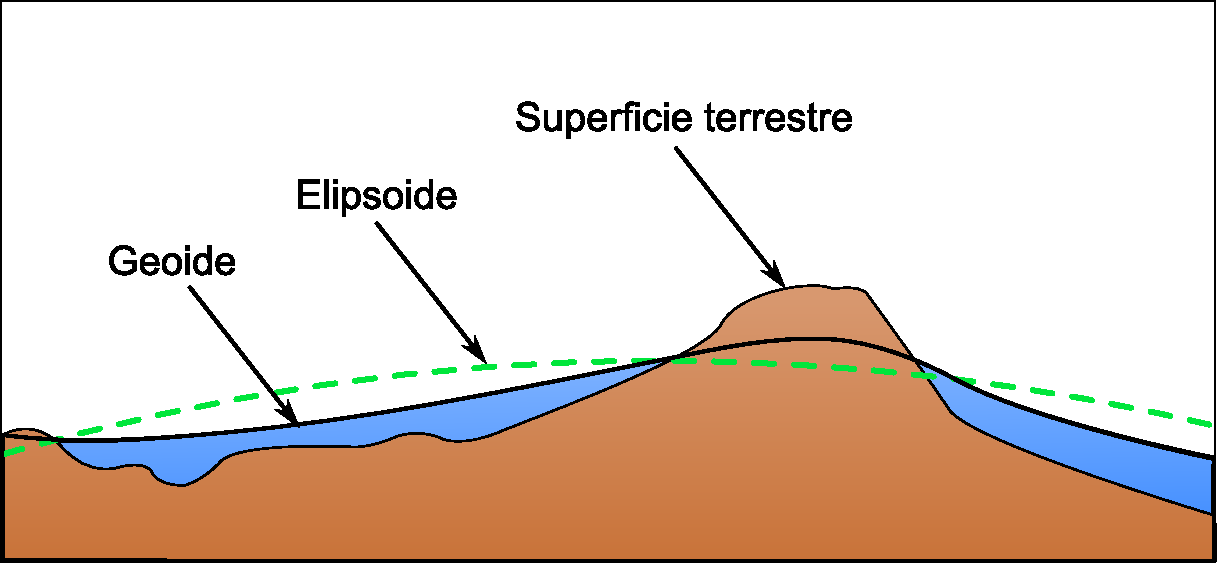
\includegraphics[width=.7\columnwidth]{../es/Fundamentos_cartograficos/Tres_superficies.pdf}
\caption{\small Tres superficies fundamentales: superficie real de la Tierra, geoide y elipsoide (Adaptado de Wikipedia).}
\label{Fig:Tres_superficies} 
\end{figure}

En un elipsoide \textbf{general}, tanto la posici�n de su centro de gravedad como de su plano ecuatorial coinciden con los terrestres. Por el contrario, cuando el elipsoide es \textbf{local}, estas propiedades no han de cumplirse necesariamente, y el elipsoide a solas resulta insuficiente, ya que carecemos de informaci�n sobre su posicionamiento con respecto a la superficie terrestre. 

Surge as� el concepto de \textbf{datum}, que es el conjunto formado por una superficie de referencia (el elipsoide) y un punto en el que <<enlazar>> este al geoide. Este punto se denomina \textbf{punto fundamental}, y en �l el elipsoide es tangente al geoide. La vertical al geoide y al elipsoide son id�nticas en el punto fundamental. 

Para un mismo elipsoide pueden utilizarse distintos puntos fundamentales, que dar�n lugar a distintos datum y a distintas coordenadas para un mismo punto.

\subsection{Sistemas de coordenadas}

Una vez hemos definido un modelo para definir la forma de la Tierra, podemos establecer un sistema de codificar cada una de las posiciones sobre su superficie y asignar a estas las correspondientes coordenadas. Para ello, encontramos dos opciones: utilizar los elementos de la \textbf{geometr�a esf�rica} y con estos definir el sistema de referencia, o utilizar la \textbf{geometr�a plana}, para lo cual ser� necesario un mecanismo de \textbf{proyecci�n} de coordenadas que permita situar los elementos de la superficie del elipsoide sobre una superficie plana.

El sistema de \textbf{coordenadas geogr�ficas} es un sistema de coordenadas esf�ricas mediante el cual un punto se localiza con dos valores angulares: \textbf{latitud} y \textbf{longitud}. Las lineas de igual latitud o longitud se denominan \textbf{paralelos} y \textbf{meridianos} respectivamente.

Las coordenadas geogr�ficas resultan de gran utilidad, especialmente cuando se trabaja con grandes regiones. No obstante, no se trata de un sistema cartesiano, y tareas como \textbf{la medici�n de �reas o distancias es mucho m�s complicada}. Para poder crear cartograf�a y simplificar gran n�mero de operaciones posteriores, necesitamos coordenadas cartesianas. El proceso de asignar una coordenada plana a cada punto de la superficie de la Tierra (que no es plana) se conoce como \textbf{proyecci�n cartogr�fica}.

La superficie de la esfera no es \textbf{desarrollable}, es decir, no puede convertirse en un plano. Por ello, es necesario disponer de una metodolog�a para pasar puntos desde la superficie curva al plano, tal y como el que se muestra en la figura \ref{Fig:Proyeccion}.

\begin{figure}
\centering
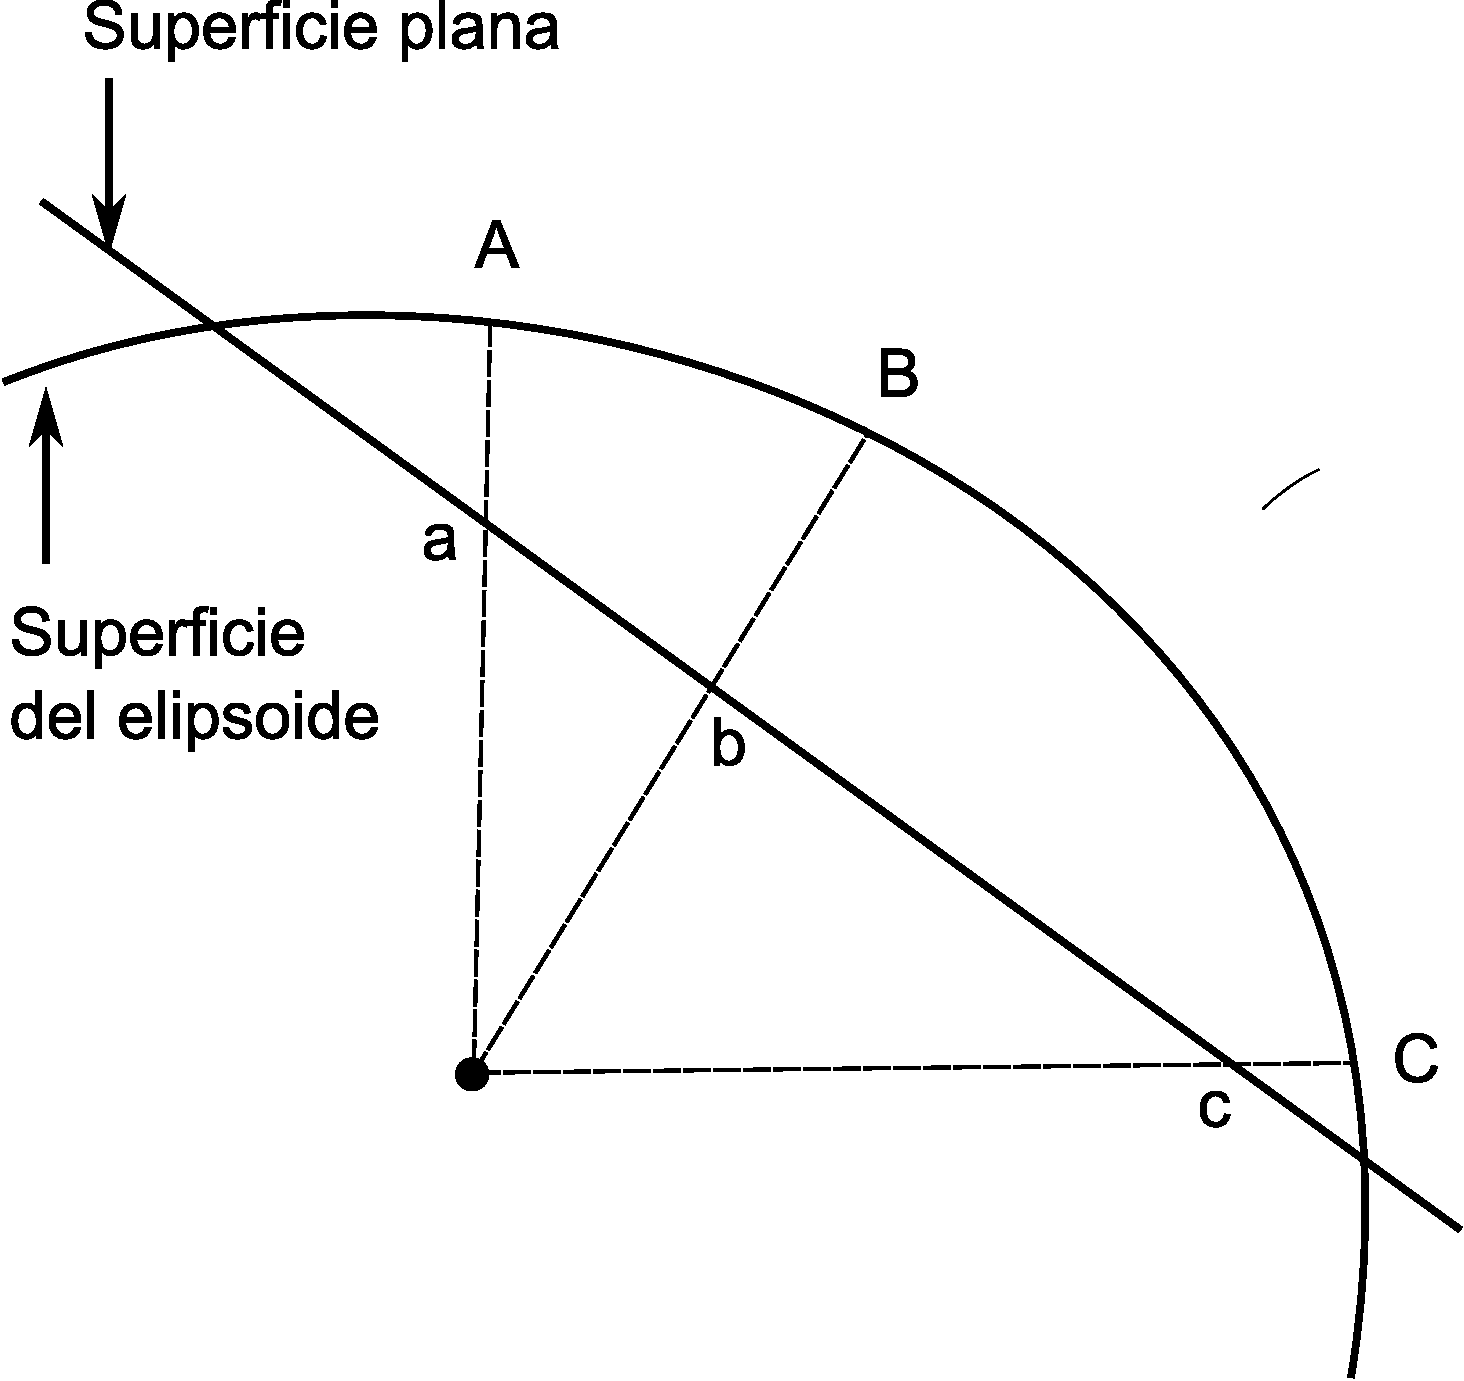
\includegraphics[width=.5\columnwidth]{../es/Fundamentos_cartograficos/Proyeccion.pdf}
\caption{\small Esquema del concepto de proyecci�n. A los puntos $A, B$ y $C$ sobre la superficie del elipsoide se les asocian equivalentes $a, b$ y $c$ sobre un plano.}
\label{Fig:Proyeccion} 
\end{figure}


En el caso de la figura, los puntos se proyectan directamente sobre un plano. Otra opci�n es proyectarlos sobre una superficie tridimensional que, al contrario que la esfera, sea desarrollable. Las m�s habituales son el cilindro y el cono, que dan lugar a las \textbf{proyecciones c�nicas} y \textbf{cil�ndricas}.

Puede apreciarse en la figura que se producen distorsiones al realizar la proyecci�n. Por ejemplo, la distancia entre los puntos $A$ y $B$ no es igual a la existente entre los puntos $a$ y $b$. Con independencia de las caracter�sticas propias de la proyecci�n, siempre existen distorsiones, por ser la de la esfera una superficie no desarrollable. Estas distorsiones se conocen como \textbf{anamorfosis} . 


Seg�n las propiedades m�tricas que se conserven, las proyecciones pueden ser \textbf{equi�rea} (mantienen una escala constante), \textbf{conformes} (mantienen los �ngulos y la forma de los objetos) o \textbf{equidistantes} (mantienen las distancias).

La elecci�n de una u otra proyecci�n es funci�n de las \textbf{necesidades concretas} de cada caso de uso. 

En la actualidad, una de las proyecciones m�s extendidas en todos los �mbitos es la \textbf{proyecci�n universal transversa de Mercator}, la cual da lugar al \textbf{sistema de coordenadas UTM}. Este sistema no es simplemente una proyecci�n, sino un sistema completo para cartografiar la practica totalidad de la Tierra. Para ello, esta se divide en una serie de zonas rectangulares mediante una cuadricula y se aplica una proyecci�n y unos par�metros geod�sicos concretos a cada una de dichas zonas. En su forma actual, emplea un �nico elipsoide (WGS--84).

Con el sistema UTM, las coordenadas de un punto no se expresan como coordenadas terrestres absolutas, sino mediante \textbf{la zona correspondiente y las coordenadas relativas} a la zona UTM en la que nos encontremos.

La cuadricula UTM tiene un total de 60 \textbf{husos} numerados entre 1 y 60, cada uno de los cuales abarca una amplitud de 6\degree de longitud. El huso 1 se sit�a entre los 180\degree y 174\degree O, y la numeraci�n avanza hacia el Este. 

En latitud, cada huso se divide en 20 zonas, que van desde los 80\degree S hasta los 84\degree N. Estas se codifican con letras desde la C a la X, no utiliz�ndose las letras I y O por su similitud con los d�gitos 1 y 0. Cada zona abarca 8 grados de longitud, excepto la X que se prolonga unos 4 grados adicionales. 

Una zona UTM se localiza, por tanto, \textbf{con un n�mero y una letra}, y es en funci�n de la zona como posteriormente se dan las coordenadas que localizan un punto. Estas coordenadas se expresan en metros y expresan la distancia entre el punto y el origen de la zona UTM en concreto. El origen de la zona se sit�a en el punto de corte entre el meridiano central de la zona y el ecuador. 

Para evitar la aparici�n de n�meros negativos, se considera que el origen no tiene una coordenada X de 0 metros, sino de 500000, y una coordenada Y de 10000000 metros, lo cual hace que todas las coordenadas referidas a �l sean positivas.

\subsection{Transformaci�n y conversi�n de coordenadas}

Una situaci�n muy habitual en el trabajo con un SIG es disponer de cartograf�a en \textbf{varios sistemas de coordenadas}, o bien en un mismo sistema pero con par�metros diferentes (por ejemplo, diferente datum). Para poder emplear toda esa cartograf�a de forma conjunta, resulta necesario trabajar en un sistema �nico y bien definido, lo cual hace necesario convertir al menos una parte de ella. Cuando el datum es distinto en los sistemas de origen y destino, la \textbf{conversi�n de coordenadas} se conoce como \textbf{transformaci�n de coordenadas}.

Las operaciones de transformaci�n y conversi�n aparecen en los SIG como funcionalidades que permiten modificar los datos geogr�ficos, reemplazando sus coordenadas por coordenadas en otro sistema de coordenadas. Igualmente, aparecen como funcionalidades de representaci�n, permitiendo la conversi�n \textbf{al vuelo}, es decir, en tiempo real. En este caso, un dato en un sistema de coordenadas se puede representar en cualquier otro sin necesidad de una conversi�n previa, con lo que puede usarse conjuntamente con datos en un sistema de coordenadas distinto.

Para facilitar el uso de sistemas de referencia, existen proyectos de codificaci�n de estos, de forma que cada sistema existente puede identificarse de forma sencilla mediante un c�digo. El m�s extendido de estos es el sistema de codificaci�n \textbf{EPSG}.

\section{Conceptos cartogr�ficos b�sicos}

De entre los conceptos fundamentales de la cartograf�a que todo usuario de SIG ha de conocer, destaca el de \textbf{escala}. La escala  es la \textbf{relaci�n de tama�o} existente entre el mapa que se obtiene al desarrollar nuestra superficie de proyecci�n (de tama�o acorde con el objeto proyectado, esto es la Tierra) y el que finalmente manejamos, de tama�o m�s reducido. Conociendo esta relaci�n podemos conocer las verdaderas magnitudes de los elementos que vemos en el mapa, ya que podemos convertir las medidas hechas sobre el mapa en medidas reales. Es importante recordar que esas medidas no son tan <<reales>>, puesto que la propia proyecci�n las ha distorsionado ---lo cual no debe olvidarse---, pero s� que son medidas en la escala original del objeto cartografiado.

La escala se expresa habitualmente como un denominador que relaciona una distancia medida en un mapa y la distancia que esta medida representa en la realidad. Por ejemplo, una escala 1:50000 quiere decir que 1 cent�metro en un mapa equivale a 50000 cent�metros en la realidad, es decir a 500 metros. Este valor se conoce como \textbf{escala num�rica}.

Independientemente del tipo de proyecci�n, la escala es completamente cierta �nicamente en determinadas partes del mapa. En otros puntos de este, la escala var�a. La relaci�n entre la escala en esos puntos y la escala num�rica se conoce como \textbf{factor de escala}. 

Aunque tradicionalmente se entiende la escala como un concepto asociado a la representaci�n, los datos geogr�ficos tienen una escala inherente que no es funci�n de dicha representaci�n, sino del detalle con que han sido tomados. En este sentido es m�s conveniente entender la escala como un elemento relacionado con la \textbf{resoluci�n} de los datos, es decir, con el \textbf{tama�o m�nimo cartografiado}. Esta concepci�n no es en absoluto propia de los SIG, ya que deriva de las representaciones cl�sicas y los mapas impresos. Se sabe que el tama�o m�nimo que el ojo humano es capaz de diferenciar es del orden de 0,2 mm. Aplicando a este valor la escala a la que queremos crear un mapa, tendremos la m�nima distancia sobre el terreno que debe medirse. 

Es importante ser consciente de la limitaci�n que la escala considerada a la hora de la toma de datos (conocida como \textbf{escala operacional}) impone, especialmente en el contexto de un SIG. En un SIG, podemos aumentar el tama�o en pantalla de una cierta informaci�n geogr�fica, variando la escala de representaci�n (tambi�n conocida como \textbf{escala cartogr�fica}), pero ello no modifica la escala operacional. Por mucho que ampliemos no vamos a ver m�s detalles, ya que para ello ser�a necesario tomar m�s datos. 

Un tipo de datos particulares con los que se trabaja en un SIG, los datos \emph{r�ster}, tienen a su vez un par�metro de resoluci�n (el \textbf{tama�o de celda}) ligado a la escala.

Relacionado con el concepto de escala encontramos la denominada \textbf{generalizaci�n cartogr�fica}. Generalizar implica expresar alguna idea o informaci�n de forma m�s resumida, de tal modo que esta sea comprensible y pueda aprovecharse de la mejor manera posible. La generalizaci�n es necesaria en un SIG para representar datos a una escala menor que su escala operacional, ya que a las limitaciones de la visi�n humana han de sumarse las limitaciones de resoluci�n que los dispositivos presentan. Por ejemplo, no tiene sentido representar el callejero de una ciudad a una escala peque�a como la que se utilizar�a para representar un mapa mundial, ya que cada peque�o punto de la pantalla contendr�a un gran n�mero de calles. Adem�s de obtener un resultado inservible, se consumir�an recursos en efectuar todos los c�lculos necesarios para producir esa representaci�n.

\begin{figure}[!hbt]
\centering
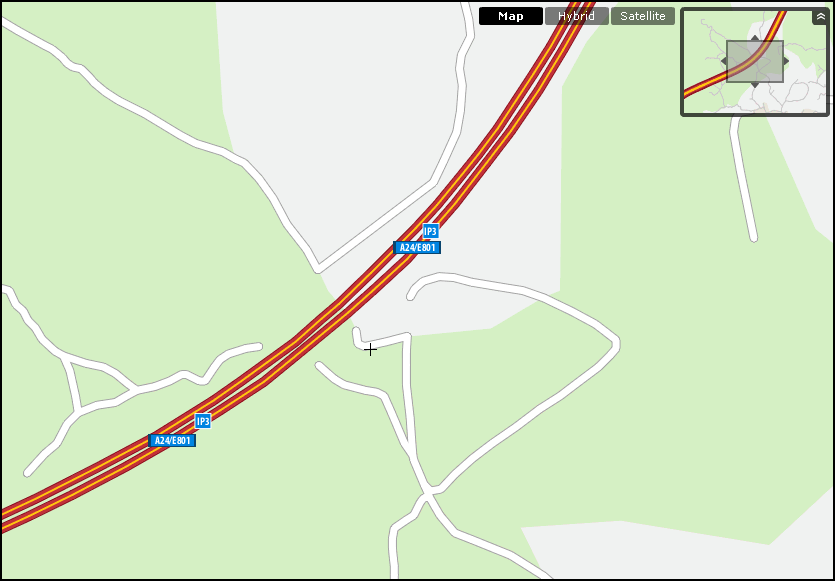
\includegraphics[width=.75\columnwidth]{../es/Fundamentos_cartograficos/Generalizacion_agregacion.png}
\caption{\small Un ejemplo de generalizaci�n por agregaci�n. Dos carreteras pr�cticamente paralelas y unidas se representan como dos elementos en el mapa, pero en el localizador de la parte superior izquierda, a escala de menor detalle, se generalizan como una �nica (Tomado de Yahoo Maps).}
\label{Fig:Generalizacion_agregacion} 
\end{figure}


En ocasiones, el proceso de generalizaci�n es necesario por razones distintas a las anteriores, y requiere operaciones tambi�n distintas. Por ejemplo, podemos crear un mapa del mundo que contenga v�as de comunicaci�n, pero no todas, sino solo las principales autopistas de cada pa�s. En este caso, no vamos a encontrar problemas con distintas carreteras que se solapan en la representaci�n, ni tampoco un volumen excesivo de datos, pero debemos igualmente <<adaptar>> la representaci�n a la escala, es decir, efectuar alg�n tipo de generalizaci�n. En este caso, se representar�an las carreteras con un ancho mayor del real, ya que, de otro modo, no ser�an apenas visibles si las representamos con su ancho correspondiente.

La generalizaci�n, por tanto, es un proceso que tiene como objetivo la producci�n de una \textbf{imagen cartogr�fica legible y expresiva}, reduciendo el contenido del mapa a aquello que sea posible y necesario representar. Para ello, se enfatiza lo que resulta de importancia y se suprime lo que carece de ella. 

Existen diversas operaciones que se emplean en el proceso de generalizaci�n. Algunas de las m�s relevantes son las \textbf{simplificaci�n} (representar un elemento menos complejo), la \textbf{agregaci�n} (representar varios elementos como uno solo ---Figura \ref{Fig:Generalizacion_agregacion}---), la \textbf{exageraci�n} (representar elementos con mayor tama�o del que les corresponde) y el \textbf{desplazamiento} (representar en una posici�n modificada, para garantizar la legibilidad). 


En un SIG, la generalizaci�n puede incorporarse como parte de los propios mecanismos de representaci�n, aplic�ndose las transformaci�n correspondientes en tiempo real. A partir de un juego de datos, se elaboran las representaciones seg�n la escala a la que se est�n representando. Esta soluci�n tiene el inconveniente de producir resultados que no resultan �ptimos, por ser la generalizaci�n un proceso complejo y dif�cil de automatizar, y, sobre todo, el de consumir gran cantidad de recursos. La generalizaci�n en este caso tiene un objetivo cartogr�fico, pero en lugar de  hacer m�s fluido el trabajo con datos de gran volumen, lo hace m�s lento.

\begin{figure}[!hbt]
\centering
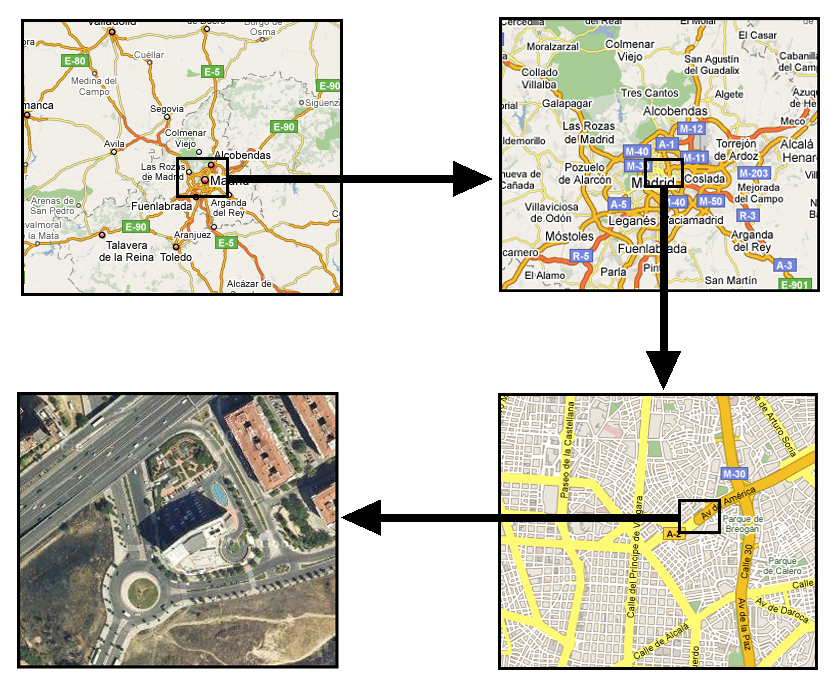
\includegraphics[width=\textwidth]{../es/Fundamentos_cartograficos/SIG_multi_escala.png}
\caption{\small En un SIG es habitual manejar informaci�n a diferentes escalas. En funci�n de la escala de representaci�n, la informaci�n visualizada ser� una u otra.}
\label{Fig:SIG_multi_escala} 
\end{figure}

Una soluci�n alternativa y m�s adecuada de incorporar la generalizaci�n dentro de un SIG suele basarse en un enfoque multi--escalar (Figura \ref{Fig:SIG_multi_escala}), en el cual se maneja informaci�n de una misma zona de estudio a diferentes escalas, y se usa en cada momento aquella que resulte m�s conveniente. Si se trabajara con cartograf�a en papel, ser�a equivalente a tener varios mapas de una zona a diferentes escalas.


El concepto de \emph{capa},\index{Capa} que veremos m�s adelante y que es vital para la idea actual de un SIG, permite este manejo simult�neo de informaci�n a distintas escalas.

En el caso de im�genes, este enfoque multi--escalar implica la creaci�n de las denominadas \textbf{pir�mides}. En lugar de una imagen con una determinada resoluci�n, se tiene una colecci�n de estas con distintas resoluciones, y en funci�n de la escala necesaria para la representaci�n, se emplea la m�s adecuada.

\pagestyle{empty}



\chapter{Geographical data}

\pagestyle{fancy}

From all GIS subsystems, the data one is probably the most important one. It is also the more interrelated, as it is linked to all of them and all depend on it to a certain extent. Data is the fuel that drives GIS. 

\section{Data and information. Types of information.}

There is a big difference between the concepts of \textbf{data} and \textbf{information}. A GIS is a Geographical \emph{Information} System, but it uses geographical \emph{data}.

Data is a \textbf{set of values of elements used to represent something}. For instance, the string 502132N is a data.

We can interpret that data as being a geographical reference, in which case it could be a latitude value, in particular 50\degree $21'$ $32''$ North. If we interpret it as being a reference to an identity card associated to a person, the information that we get from it is completely different. It is the same data, containing six digits and a letter, but the information that we extract from it is different, since we understand and interpret it in a different way.

Information is, therefore, the result of data and \textbf{its interpretation}. and in many cases, working with data means just trying to extract from it all the information that it might contain.

Understanding the meaning and the differences between data an information allows us to understand, for instance, why the ratio between the size of a given data and the amount of information it contains is not constant. The strings 502132NORTH and FIFTY TWENTY ONE THIRTY TWO NORTH are longer than 502132N, but they contain the same information (as long as we interpret them as the latitude component of a coordinate).

Geographical information has two separate components: \textbf{spatial} and \textbf{thematic}. The spatial component contains the position, referred to a given reference system, and it answers the question \emph{where?}. The thematic component answers the question \emph{what?}, and it defines the characteristics of the phenomenon or feature that occurs at the location indicated by the spatial component.

While the spatial component is usually a numerical value (most coordinate systems use just numbers), the thematic component can be \textbf{numeric} or \textbf{alphanumeric}. A numeric variable can be itself of four different types: \textbf{nominal, ordinal, interval} or \textbf{ratio}.

The operations that can be performed on a certain geographical data are defined by the types of variables contained in its thematic component.

The different approaches for representing and storing geographical information, which we will see later in this same chapter, depend on the type of variable that we are working with.

An important concept to consider related to geographical information is the \textbf{dimension}. The elements that we store range from simple points (0D), to three-dimensional volumes (3D) (Figure \ref{Fig:Dimensions}).

\begin{figure}[!hbt] 
\centering
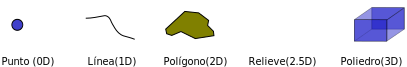
\includegraphics[width=\textwidth]{Data/Dimensions.pdf}
\caption{\small Dimensions of the spatial component of geographical data.}
\label{Fig:Dimensions} 
\end{figure}


\section{Subdivision of information. Layers}

In a GIS, the information about a given study area \textbf{is divided in several levels}. Even if it refers to the same location, the information about different variables is stored separately. That is, a set of different blocks of information exists for the same area, each of them containing a particular variable or set of elements. Each of these blocks is called a \textbf{layer}.(Figure \ref{Fig:Concept_layer}). 

\begin{figure}[!hbt] 
\centering
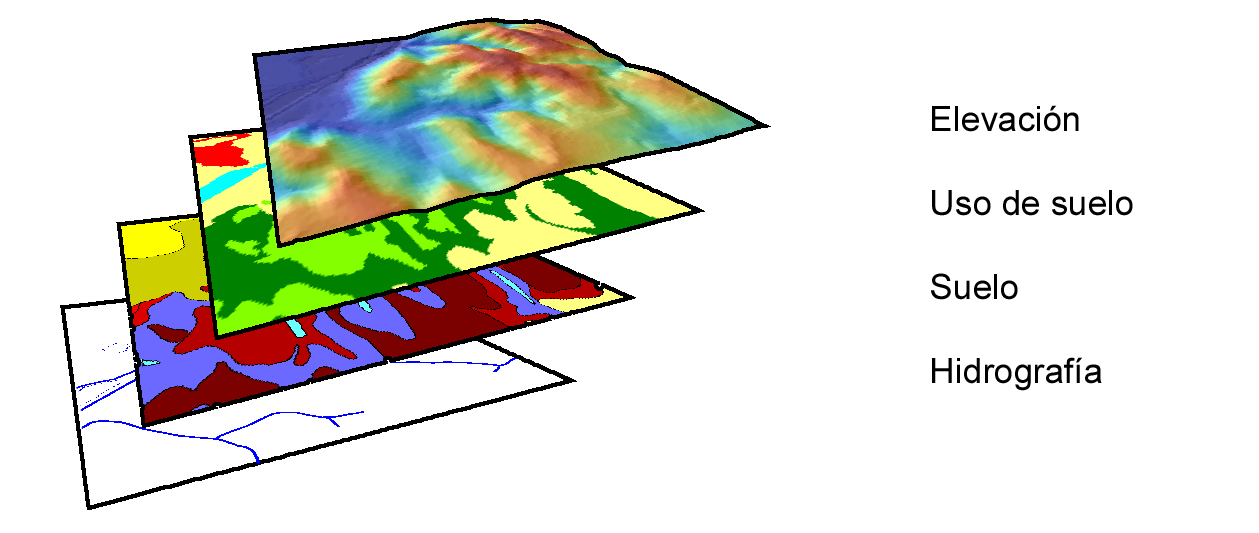
\includegraphics[width=\textwidth]{Data/Concept_layer.png}
\caption{\small A graphical explanation of the concept of \emph{layer}.}
\label{Fig:Concept_layer} 
\end{figure}

The concept of layer is fundamental to understand GIS, and it helps to correctly structure and manage geographical information. All the information that we will use in a GIS will be in the form of layers. Each one of them can be used independently or along with others.

With traditional cartography, it is not possible (or it is complex and not accurate) to combine different types of information, such as, for instance, the one contained in a topographic map and the one from a land-use map. In the case of a GIS, the different layers in which that information is contained can be combined in an easy and clean way.

The concept of layer as the fundamental unit for geographical information in GIS has a huge relevance, as it constitutes the basic framework for most operations. For instance, we saw in the section about cartographic generalization how in a GIS we can use different <<versions>> of the data corresponding to a given area, and show one or another depending on the current scale. This versions will be stored as independent layers. Layers are, thus, not just the fundamental unit for a given area, but also for a given scale, and allow to optimally separate and organize geographical information. 

Layers also help avoiding data redundancy, since each layer just contains information about a particular variable or type of feature. A traditional map always contains a set of different variables, not just a single one. Some of them are used to provide a general context, such as the names of the main cities or the main roads, and these appear in most maps. In a GIS, they exist independently, and the user can add them and combine them with other layers whenever is needed. Therefore, working with layers provides a more efficient approach and a \textbf{more atomized} organization of the data, with the advantages that it has for its storage, management and use.

Apart from dividing geographical information in layers depending on its content, it is also divided considering purely spatial criteria, <<cutting>> it in smaller parts that cover a smaller area. This is similar to what happens with traditional cartography, divided in \textbf{map sheets}.

The main feature of a GIS to transparently integrate data corresponding to different areas and create a seamless mosaic is the \textbf{separation between the data and its visualization}. Data is required for visualization, but these two elements constitute different parts of a GIS, with a clear separation between them. That means that data is used to create a visual output, but data itself does not contain any value related to its rendering and visualization.

Thus, it is possible to combine data and then represent that combination together as a whole. Something like that is not possible with a printed map, since it contain also the visualization elements (colors, line thickness, label placements, etc.) and even some additional cartographic ones (legend, scale, North arrow, etc.). Even if printed maps can be combined, information contained in them does not <<fuse>> to create a single new map. In a GIS, on the other hand, visualization of several blocks of data can be identical to the one that would be obtained if that data were stored as a single block.


\section{Geographical information models}

The process of converting a given geographical area and the information about it in a data that can be used within a GIS can be divided in three different phases.

\begin{itemize}
 \item Establishing a \textbf{geographical model}. That is, a conceptual model of a reality and its behavior.
\item Establishing a \textbf{representation model}. That is, a way of coding the conceptual model, reducing it to a finite set of elements.
\item Establishing a \textbf{storage model}. That is, a storage strategy for storing the elements of the representation model.
\end{itemize}

Representation models are the most important ones, and we will focus on them here. The two main representation models are the \textbf{raster model} and the \textbf{vector model}. Layers using these models are commonly known as \textbf{raster layers} and \textbf{vector layers}.

\subsection{Raster model}

The raster model is based on a \textbf{systematic division of space}. The whole space is characterized by a set of elements that cover it, each of them with an associated value.

The most common raster model is based on a grid of \textbf{square cells}, or sometimes rectangular ones. Knowing the orientation of the grid, the size of  the cells (which is the same for all of them), and at least the coordinates of one of them, it is possible to know the location of all cells, thanks to its \textbf{regular structure}. With that, the values of the variable we are working with are known in all points of the area that is covered by the layer. The \textbf{cell size} is a parameter related to the scale of the layer, since it defines its resolution and depends on the level of detail used when the corresponding measures were taken.

Figure \ref{Fig:Raster_closeup} shows an example of a raster grid.

\begin{figure}[!hbt]   
\centering
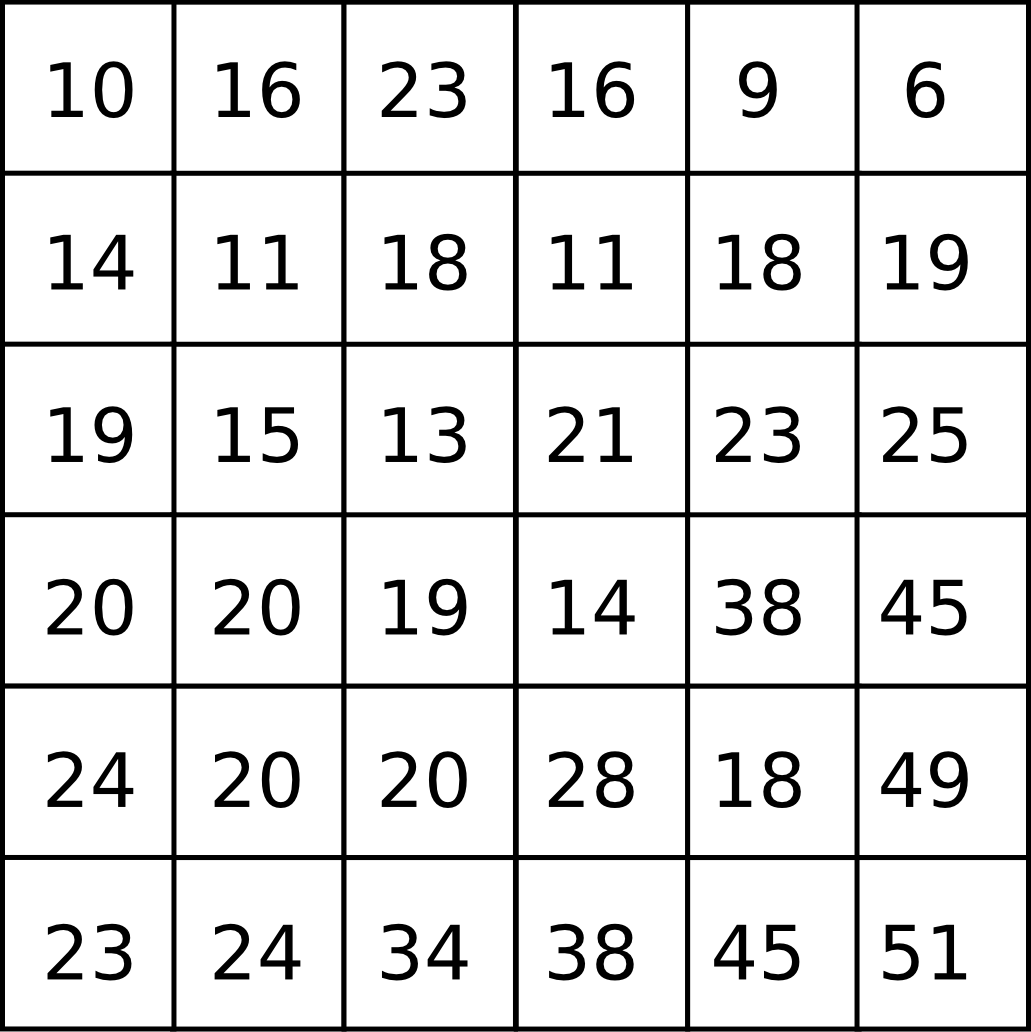
\includegraphics[width=.4\textwidth]{Data/Raster_closeup.png}
\caption{\small Cells in a raster grid with their associated values.}
\label{Fig:Raster_closeup} 
\end{figure}

The number of values stored for each cell defines the number of \textbf{bands} in a raster layer. A band contains a single value for each cell. We can understand a raster layer with more than one band as a set of sublayers, all of them having the same spatial structure (extent and cell size), and wrapped as a single layer.

We can find a clear example of that in digital color images. A digital image is composed of a grid of values (called \textbf{pixels}), each of them with an associated color. In the most common case, that color is expressed with three values, corresponding to the intensity of colors red, green and blue, which, when combined, give the pixel color. That is, an image like that is a raster layer with three bands, containing each of them one of the red, green and blue components.

Another typical use of the raster model is for the so-called \textbf{Digital Elevation Models} (DEM), which contain the topography of a given area. These are always single band layers.

In most cases, the values of a raster layer are numerical, and GIS software is usually not adapted to handle other types of values in the thematic component of a raster layer. Due to this, raster layers can be seen as \textbf{matrices}, and the corresponding mathematical tools can be used for their analysis.


\subsection{Vector model}


The other main representation model is the vector model. In this model, there are no fundamental units that divide and cover the area that is modeled. Instead, the variability and characteristics of that area are modeled using \textbf{features}, which represent elements in which those characteristics do not change. The geographical part of a feature is made of \textbf{geometric primitives}, and these can be of three different types: \textbf{points}, \textbf{lines} and \textbf{polygons} (Figure \ref{Fig:Primitives}).

\begin{figure}[!hbt]   
\centering
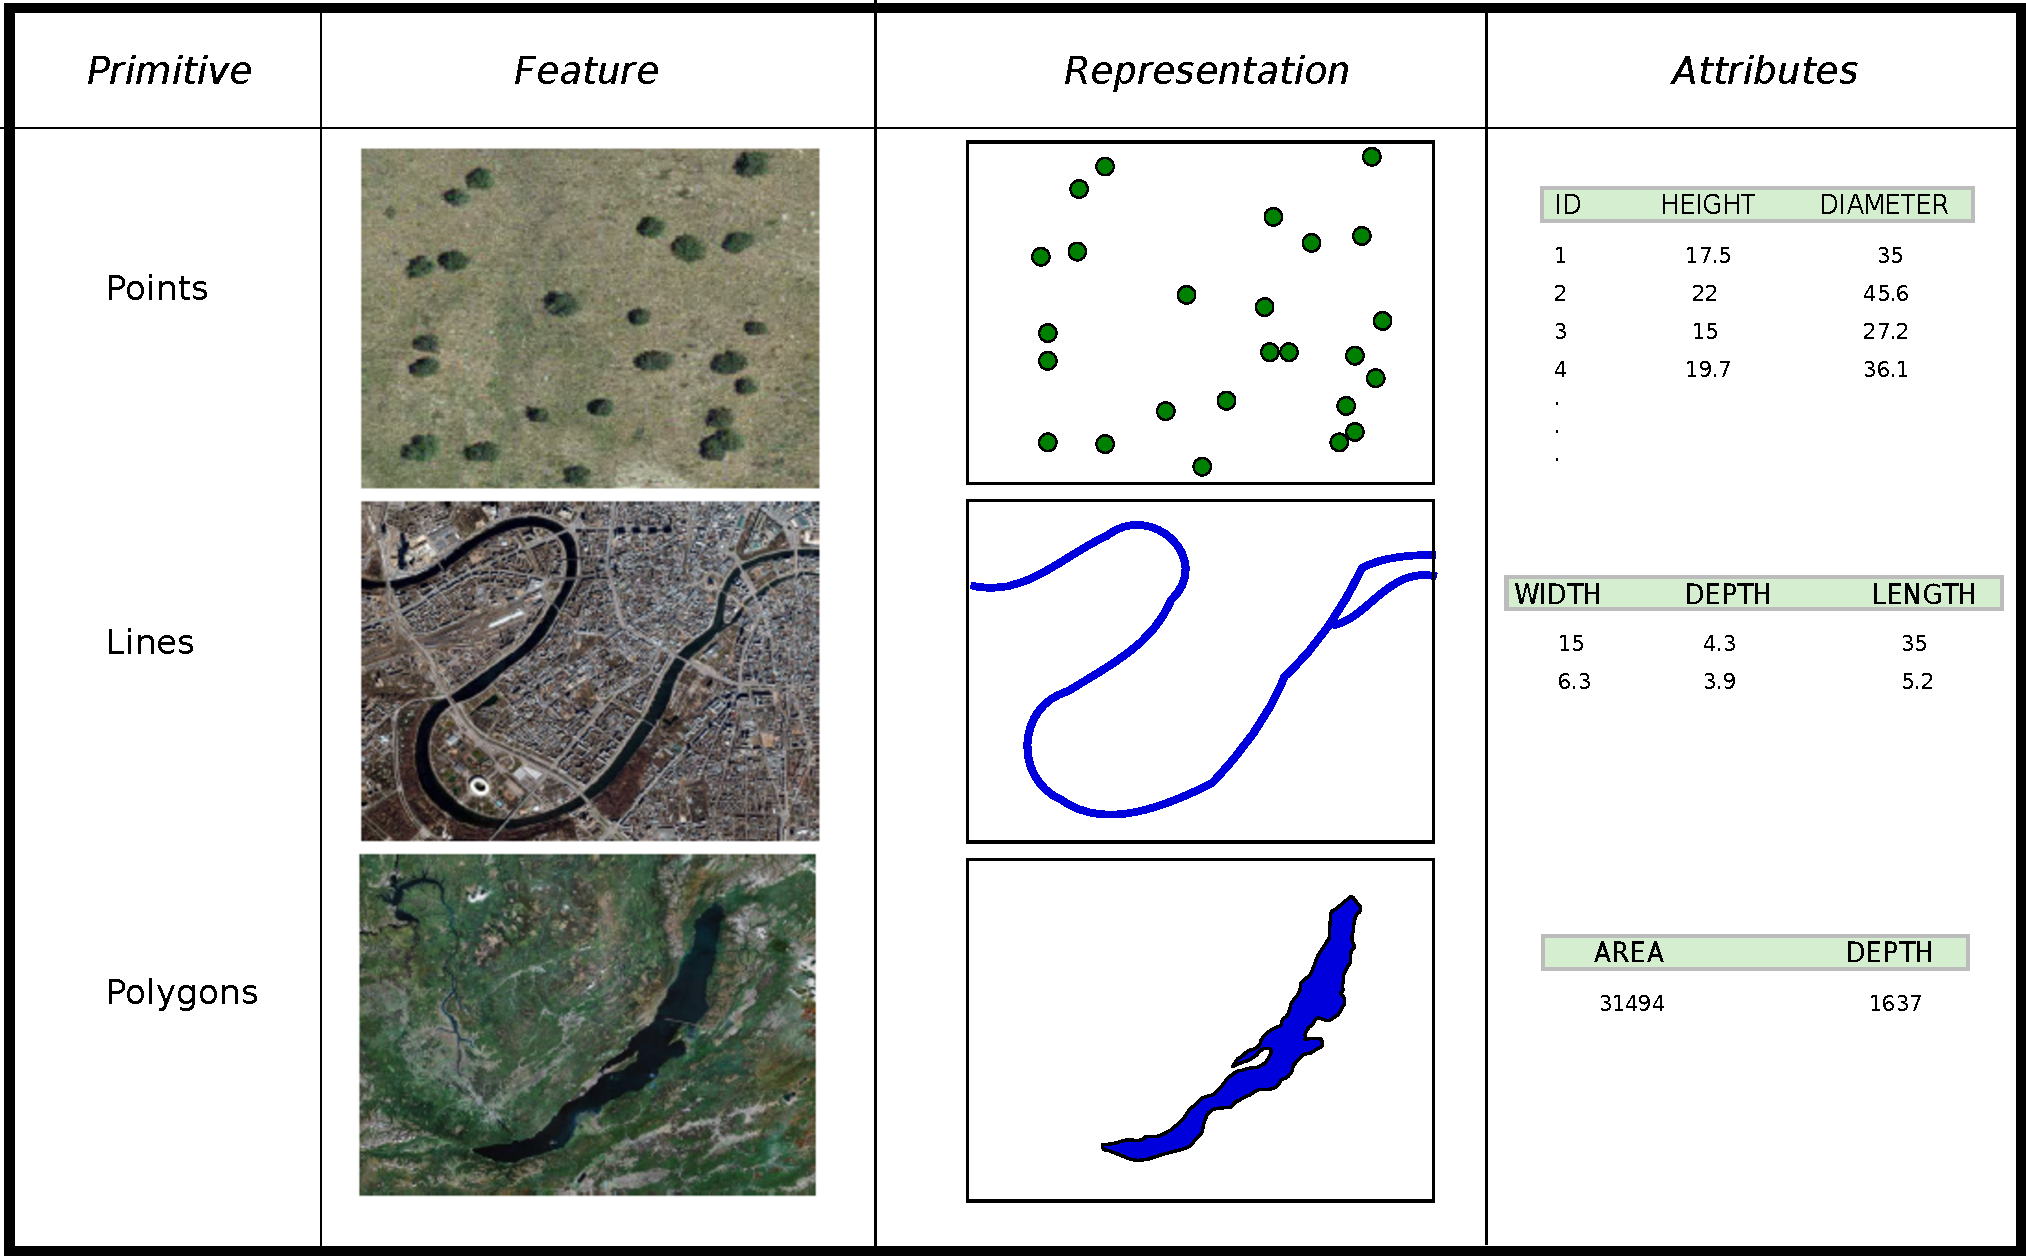
\includegraphics[width=\textwidth]{Data/Primitives.pdf}
\caption{\small Geometric primitives in the vector representation model and some examples of each of them and their associated attributes}
\label{Fig:Primitives} 
\end{figure}

Using points, lines and polygons, geographical space can be modeled by associating values to these primitives. A feature can have \textbf{multiple primitives}. For instance, in a layer that contains countries, a country such as the United States will require several polygons (continental US, Alaska, Hawaii islands, etc.). All those polygons form a single feature, since all of them belong to the same country and will share the same associated values.

A layer can contain features with primitives of different types, but usually it is restricted to just one single type. It is common to speak of a <<points layer>> or a <<polygons layer>> to indicate that. 

Elements can be represented using different types of primitives. For instance, a city can be represented as a single point or as a polygon with its perimeter. Using one or another geometry should depend on the type of phenomenon that we want to model or the level of detail that is needed, among other factors.

The thematic component in the vector model is defined using \textbf{attributes}. A layer usually contains multiple attributes. Attributes are associated to features, can have information of all types, and they are more versatile than the values associated to raster layers, which, as it was mentioned, normally contain just numerical values. Due to its particular structure (a set of attributes associated to a feature), the thematic component in the vector model can be represented as a table and stored in a \textbf{database} (we will see more about this in the chapter devoted to databases). Also, it can be be analyzed independently of the spatial component.

A particular element of the vector representation model is \textbf{topology}. A vector layer is said to contain topology if it contains the spatial relations between its features. Topology is required for certain analysis, and changes the way some operations, such as geometry editing, work in a GIS.

\begin{figure}[!hbt]   
\centering
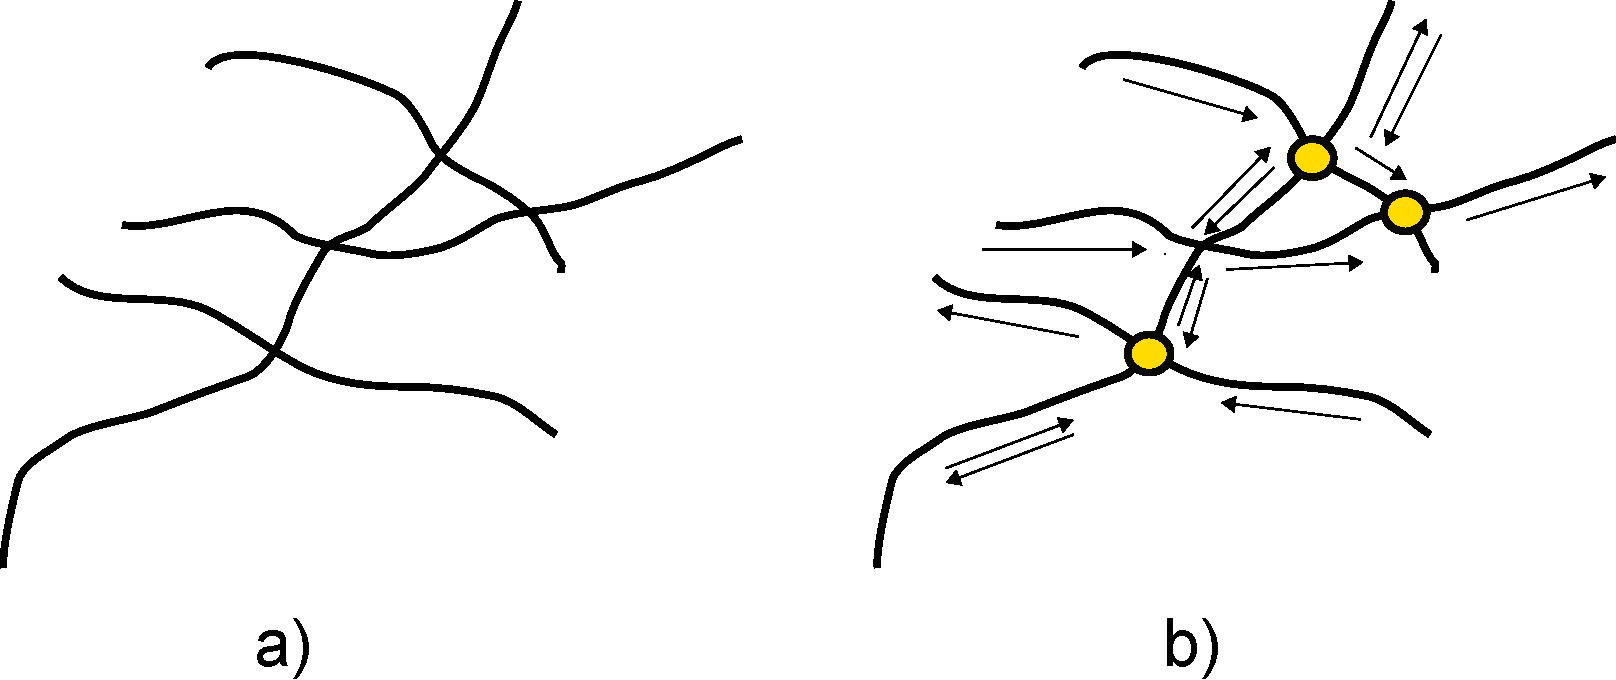
\includegraphics[width=.8\columnwidth]{Data/Topology_roads.pdf}
\caption{\small A roads layer without topology (a) and with topology (b). Circles in this last case indicate connections between roads.}
\label{Fig:Topology_roads} 
\end{figure}

Although most vector layer operations can be performed without topology, some of them such as \textbf{network analysis} are not possible without it. If we think about a roads layer, if it just contains lines representing roads but no information about how they are connected, there is no way of constructing the network from them. The points where lines intersect might be crossings or roundabouts (so it is possible to move from one road to another), but they might also be points without connection between the roads (one passing above the other). Without knowing that, we are missing information, and the network analysis cannot be performed. (Figure \ref{Fig:Topology_roads})

Line data without topology is popularly know as \emph{spaghetti} data.


\subsection{Raster \emph{vs} vector}


Both the raster and vector representation models can be used to store \textbf{any geographical information}. Figure \ref{Fig:Representation_models} contains an example of that, and it shows a roads layer represented using both models. 

We mentioned DEMs as a typical case of raster layers. Representing elevation as a raster layer has many advantages, especially for performing analysis, but it is not the only option. We can have a vector layer with points (that will be the case if the elevation data comes for a topographic survey), or a lines layer with contour lines (which is the most common way of representing elevation in a traditional map).

\begin{figure}[!hbt]   
\centering
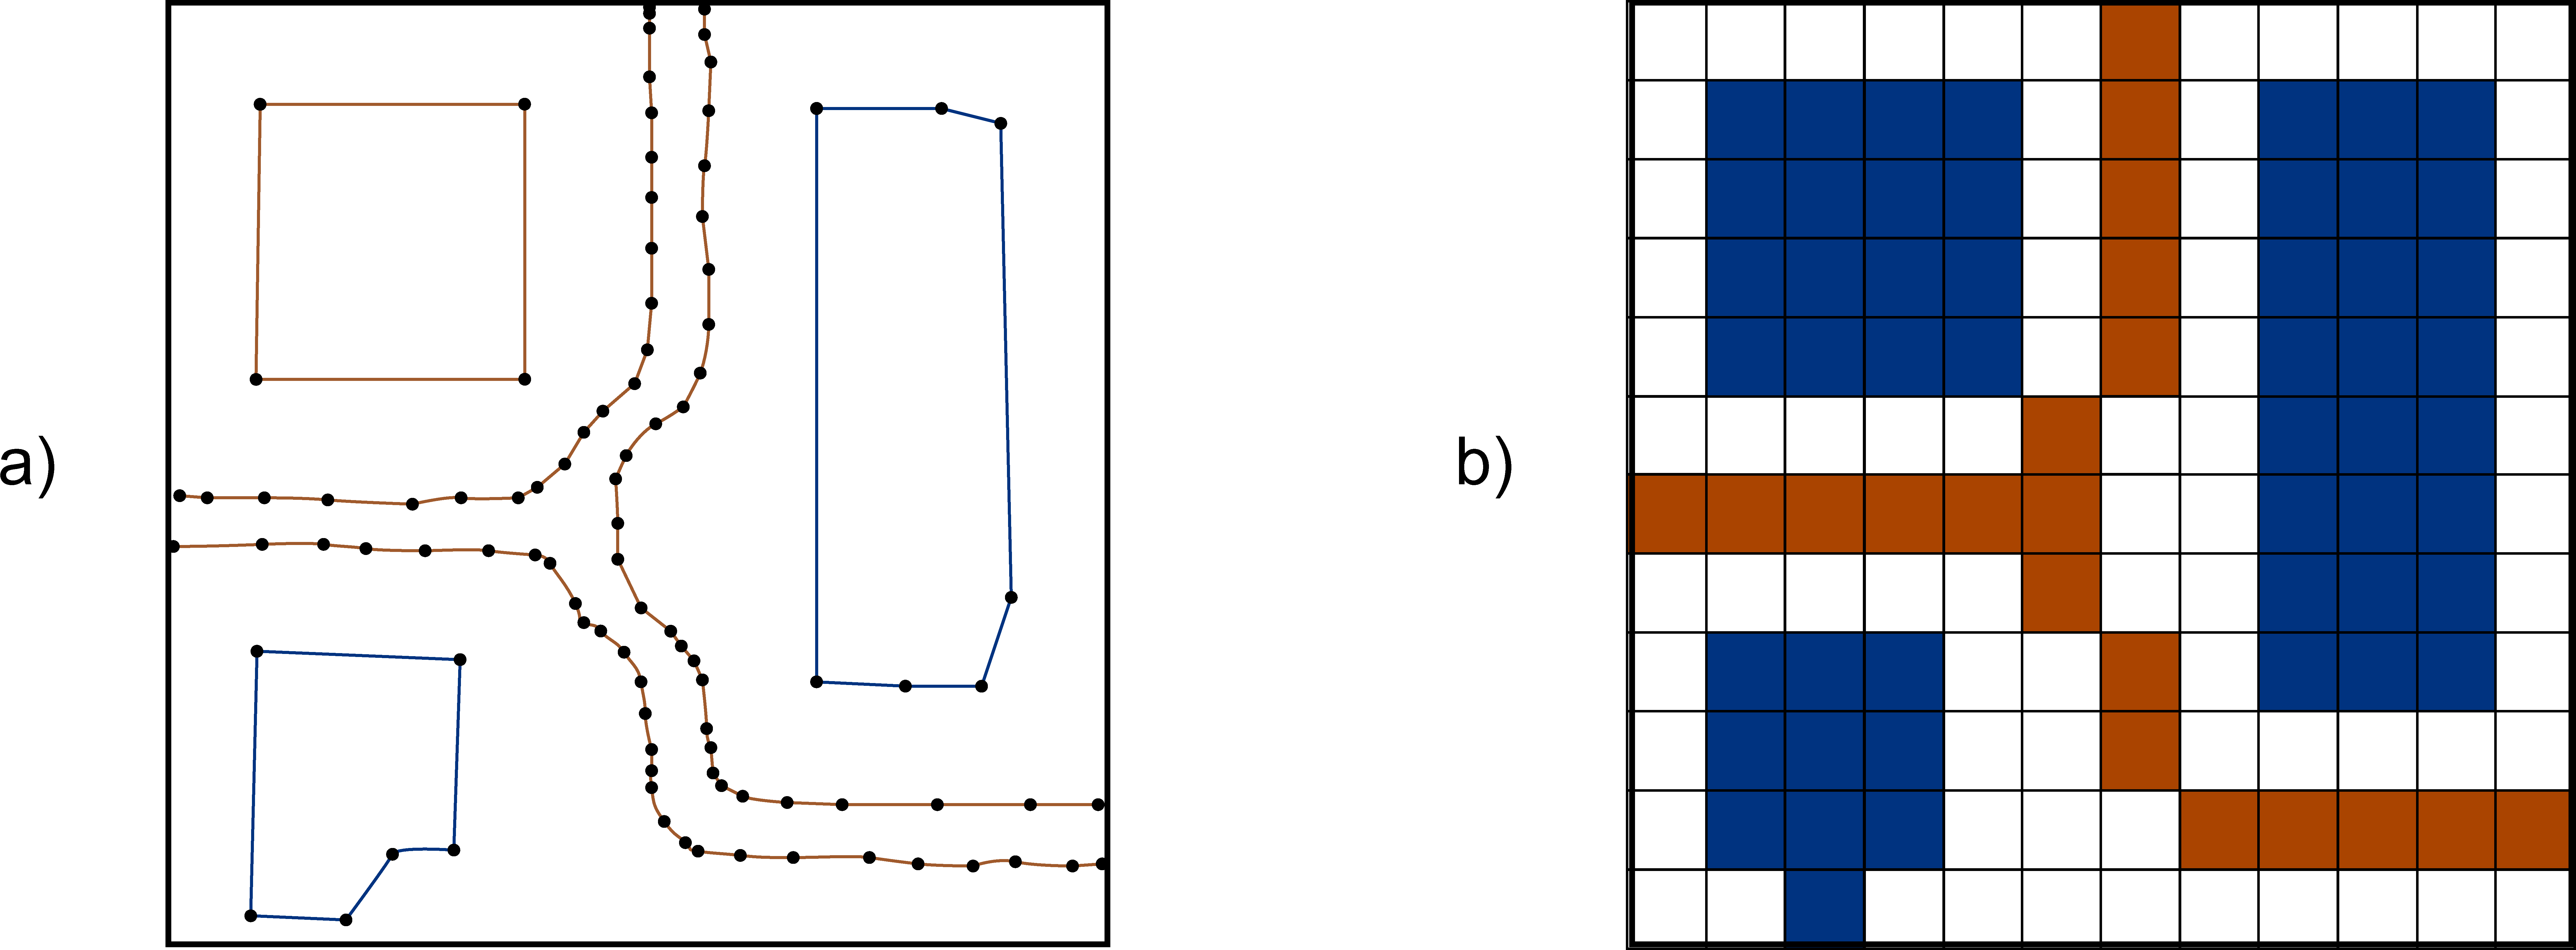
\includegraphics[width=\textwidth]{Data/Representation_models.pdf}
\caption{\small Comparison between vector (a) and raster (b) representation models.}
\label{Fig:Representation_models} 
\end{figure}

It is clear that both models have many differences, and each of them has it pros and cons. The following are some ideas to compare between them.


\begin{itemize}
\item \textbf{Approach}. Raster model focuses on the properties of the space that is represented (\emph{what} and \emph{how}), while the vector model focuses on the location of that property (\emph{where}).
 \item \textbf{Accuracy}. Raster model has its precision limited by the cell size. While this can be as small as we want, that would result in very large amounts of data. Features smaller than that size cannot be represented, and it is assumed that there is no variability within a cell.

 Also, shapes are limited to straight angles, since the base unit for the raster grid, as we have seen, it is a square or rectangle (Figure \ref{Fig:Raster_accuracy}

\begin{figure}[!hbt]   
\centering
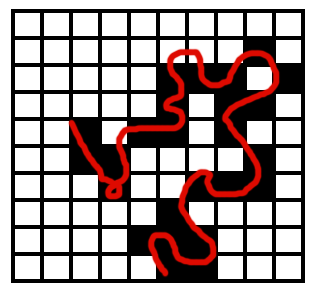
\includegraphics[width=.4\columnwidth]{Data/Raster_accuracy.png}
\caption{\small Limitations of the raster representation model. Since the space is divided in square units, elements such as curves cannot be faithfully represented.}
\label{Fig:Raster_accuracy} 
\end{figure}

\item \textbf{Complexity}. Analysis algorithms, specially those in which several layers are used and combined, are usually simpler and easier to implement with raster layers, mainly due to their regularity and systematicity. Working with vector layer, which do not have any regularity, tends to be more complex from the algorithmic point of view.
\end{itemize}

Overall, there is no representation model that is better than the other. Depending on the case, one will be more suitable than the other. The following factors should be considered when evaluating the suitability of these models to a particular circumstance:

\begin{itemize}
 \item \textbf{Type of variable or phenomenon to represent}. In general, it is better to use raster layers for \textbf{continuous} variables such as elevation, in order to make it easier to perform analysis based on them. \textbf{Discrete} variables, on the other hand, are better represented using a vector approach.
\item \textbf{Layer purpose}. It is important to know how we plan to use a layer, to decide the representation model that might better suit our case. For instance, if we have elevation data and we plan to perform analysis, it will be better to have a raster DEM, since most algorithms require the elevation data to be raster layer. However, if we want to use that elevation data just for visualization and combine it with other layers to create a map, it might be better to have a vector layer with contour lines, since those will be a better cartographic solution and will interfere less with the remaining variables. 
\item \textbf{Context}. The context might make it better (or even mandatory) to work with a given representation model. For instance, if we are working with images and we plan to do some analysis with other layers as well, those should be raster ones, since images, as we have seen, are always raster layers.
\end{itemize}

There are algorithms that allow \textbf{converting between the raster and vector representation models}, so if we have our data in one of them, we can obtain a new layer that uses the other model and might be more suitable for our work.

\pagestyle{empty}

\chapter{Geographical data sources}

\pagestyle{fancy}

Not so long ago, all information used in a GIS came had its origin in a paper map, which was \emph{prepared} to adapt to the particular nature of that GIS. Geogrpahical data were obtained from the \textbf{digitalization} of printed cartography, that is, from the conversion of analogic maps into digital data that a GIS can handle.

Apart from the fact that we can use them in a GIS, digital data have many advantages and represent an important qualitative imrpovement. Digital data are easier to update, easier to distribute (specially since the Internet was created), use less physical space and are easier to maintain (digital data do not degrade. Their physical support does, but they are easy to replicate without losing their quality).

Techniques for gepgraphical data aquisition have evolved, and can now create data that can be directly integrated into a GIS. Data sources that produce data ready for being used in a GIS are called \textbf{primary} data sources. Those that generate data that has to be adapted or converted are called \textbf{secondary} data sources.

In this chapter, we will see the main data sources that provide data for GIS.

\section{Remote sensing}

Remote sensing is the \textbf{acquisition of information about an object or phenomenon without making physical contact with it}. Instead of measuring the object itself, it measures the perturbations ---mainly the electromagnetic ones--- that it causes on its surroundings. In our case, it is applied to objects on the Earth's surface.

A remote sensing system contains the following elements (Figure \ref{Fig:Elements_remote_sensing}):

\begin{figure}[!hbt]   
\centering
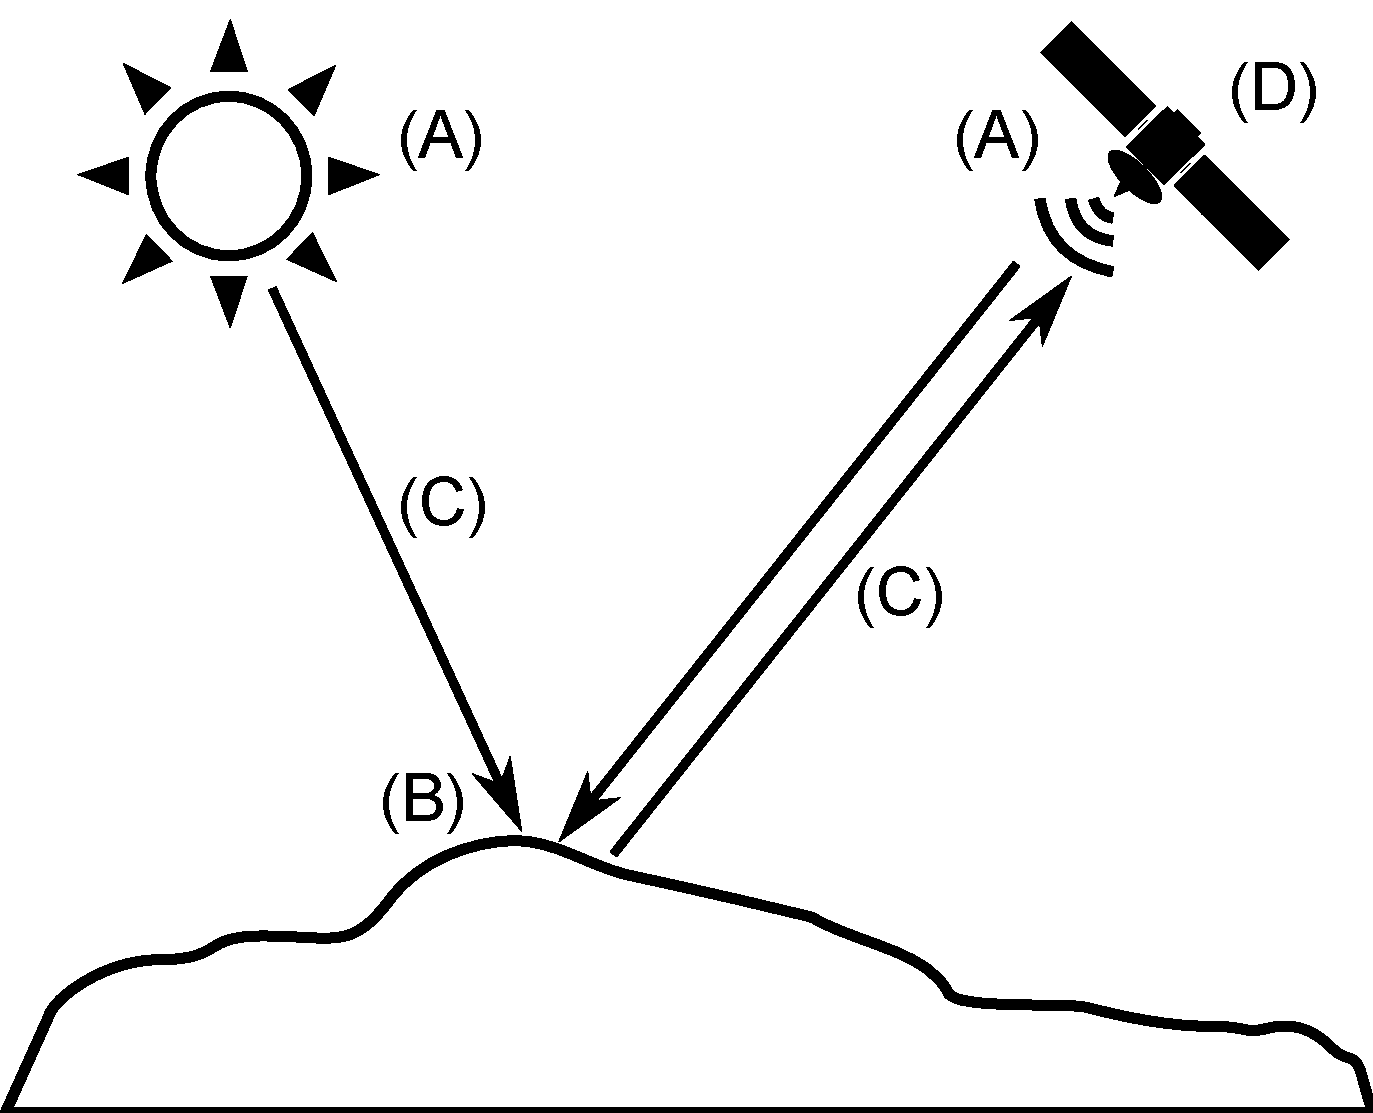
\includegraphics[width=.6\textwidth]{Data_sources/Elements_remote_sensing.pdf}
\caption{\small Elements in a remote sensing system.}
\label{Fig:Elements_remote_sensing} 
\end{figure}


\begin{itemize}
	\item \textbf{A source of radiation (A)}. It can be natural or artificial. Radiation emitted by the source reaches the Earth's surface and is altered by the presence of the objects on that surface. Remote sensing studies that alteration. Objects themselves can emit radiation as well.
	\item \textbf{Objects (B) that interact with radiation} or can emit it, as mentioned above.
	\item \textbf{An atmosphere (C)} through which radiation moves from the source to the objects. The atmosphere also interacts with the radiation and alters it.
	\item \textbf{A receiver (D) which receives the radiation} once that has been emited or altered by the objects. The receptor measures the intensity of the radiation coming from differnt points in the area being studied, and with them generates its final product (in most cases, and image). 
\end{itemize}

In this chapter, we will describe these elements in detail. To study the two first, we will also study some fundamentals about radiation and its interaction with matter. For describing the receivers take make part of a remote sensing system, we will separate them into two components: sensors and platforms.

Interaction with the atmosphere is interesting in order to eliminate its influence, since in most cases we are interested in the object on the Earth's surface, not the atmosphere itself. Removing that influence is part of the post-processing of the data. Those processes are, however, rather complex, and they will not be explained here.


\subsection{Electromagnetic radiation}

Electromagnetic radiation is caused by alterations in the electric and magnetic fields, which generate waves corresponding to each one of the. This waves move at the speed of light and can be described with the usual parameters such as wavelength and frequency. The range of frequencies (and corresponding wavelengths) of electromagnetic radiation is calle the \textbf{electromagnetic spectrum}

The spectrum is subdivided in regions depending on the wavelength, such as (for shorter to larger wavelength) gamma rays, X rays, ultraviolet region, visible region, infrared region or microwaves.


Radiation emited by a radiation source is altered by the presence of objects that \textbf{absorb, transmit} or \textbf{reflect} it.

These three phenomena take place in a different proportion depending on the characteristics of the object and the radiation. For remote sensing, \textbf{the interesting part fis the one that is reflected}, since it is the one that can be collected later and used to produce the data output.

Since each object reflects radiation at different wavelengths in a different way, this can be considered as a property of an object. The particular response of a given object and the way it alters a given radiation (which depends on its shape, material, etc.) is known as its \textbf{spectral signature} and can be used to identify the object.


\subsection{Sensors and platforms}

The two main technological elemtns in a remote sensing system, both of them related to the receiver are the \textbf{sensor} and the \textbf{platform}.

The sensor is the element that can <<read>> the electromagnetic radiation and register its intensity for a given zone of the spectrum. It can be a simple photographic camera or a more specialized sensor.

\textbf{Passive} sensors use natural source of radiation (in most cases, sunlight), and just measure that radiation as it is reflected on the Earth's surface. \textbf{Active} sensors emit their own radiation, and then collect it back after it has been reflected. Here is a simple example to better understandthis: a photographic camera as a passive sensor, while a photographic camera that uses a flash unit is an active one. The radiation emitted by an active sensor does not have to be visible light (as in the case of the flash); the sensor can emit in other parts of the spectrum.

Technologies such as \textbf{radar} or \textbf{LiDAR} (similar to radar but with light pulses instead of radio waves) are based on active sensors.

The sensor is \textbf{mounted on a platform}, and it perfoms its data acquisition from it. \textbf{Several sensors} can be mounted on a single platform.

The two main types of platforms are those located inside the Earth's atmosphere (mostly on airplanes) and those outside of it (on satellites).

The advantage of airplanes is their \textbf{availability}, since they can be piloted and used to cover any place on earth at any moment. Satellites, on the other hand, cannot be guided, and its movement is fixed and defined by a set of parameters known as \textbf{orbital parameters}, which define the orbit described by the satellite around the Earth.

Orbits can be classified according to their \textbf{rotation axis} or their \textbf{movement}. Two particular cases are the \textbf{geosynchronous} orbits (the satellite is located in a fixed point and its movement follows the earth rotation) and the \textbf{heliosynchronous} (the satellite passes over any given point in its path always at the same local solar time).
	
\subsubsection{Resolutions}

One of the most important parameters that define the characteristics of a remote sensing system are its \textbf{resolutions}. These define the level of detail of the products that it creates. Resolutions depend on both the sensor and the platform as an single operative unit, and on the individual characteristics of each of them. Four resolutions can be defined:

\begin{itemize}
	\item \textbf{Spatial resolution}. It indicates the size of the smaller object that can be distinguished. If the output is an image, the spatial resolution is the real size of the area represented by a single pixels.
	\item \textbf{Spectral resolution}. It indicates the amplitude of each of the regions of the spectrum that is registerd. It is defined by the total amplitude that is covered and the number of sections into which it is divided. The measurement corresponding to each of these sections will usually be stored in a separate band in the resulting image. 
	\item \textbf{Radiometric resolution}. It indicates the level of detail of the intensity measurement taken for each of the spectral regions that are registered. 
	\item \textbf{Temporal resolution}. It indicates the time that it takes the sensor to return to a given place. It makes sense only for orbital sensors. It depends on the platform characteristics, such as its attitude, and also on the sensor characteristics.
\end{itemize}

It is not possible (for technical or theoretical reasons) to have a sensor in which all the above resolutions are high. Some sensor might favor cetain resolutions, while other might favor different ones.

When using images coming from remote sensing in a GIS, we should consider which resolution is more important (for instance, to locate elements that have a small size, high spatial resolution is needed). Using data from several different sensors is a good strategy for overcoming these limitations.


\subsection{Photogrammetry}

Photogrammetry is the technique used to study and precisely define the shape, size and position in space of any object, using measurements taken on one or several photographs. Of special interest to GIS is the branch of photogrametry known as \textbf{aerial photogrammetry}, which uses aerial photographs and it is mainly used for generating elevation data through a process known as \textbf{restitution}.

Instead of single images, the branch of photogrammery known as \textbf{stereophotogrammetry} uses pairs of images, each of them taken from a different point. These images form a \textbf{stereo pair} and with them a three-dimensional reconstruction of the original scene can be produced. This can be used by an operator to <<see>> the scene with \textbf{depth and volume}, and using that, terrain forms can be identified and elevation information can be obtained. 

If using satellite images, stereo pairs can be obtained from those platforms and sensors that allow \textbf{changing the angle of vision}, so in the same satellite pass pictures of a given area can be taken from different points.

Photogrammetry can be \textbf{analogic} or \textbf{digital}, the latter being the one more related to the field of GIS.

Stereoplotters are used to combine and align the images that form the stereo pair. Current stereoplotters are called \emph{analytical stereoplotters}  contain elements from GIS, along with more specific ones. Among these, we find specific visualization software and peripherals such as 3D mouses or other mechanical elements found in analogic photogrammetric devices, making it easy for operators to adapt to this new type of tools.

\section{Printed cartography. Digization}

A large amount of cartography exists in printed form, such as maps or old analogic aerial photographs. To be used in a GIS, this cartography has to be \textbf{digitized}. That means creating raster or vector layers from them. In this last case, it also implies \textbf{separating the different types of information} that the map might contain, since printed maps information that, in a GIS, would be stored in independent layers.


Digitizing a printed cartographic document involves three steps: 

\begin{itemize}
\item \textbf{Georeferencing} the original document. That is, setting a geogrpahical context (coordinate system, control points, etc.), so the digitized element that we will produce are correctly referenced.
\item \textbf{Digitizing the spatial component}. That is creating the corresponding geometries.
\item \textbf{Digitizing the thematic component}. Creating cell values for raster layer or attributes in the case of vector ones.

Digitazion can be \textbf{manual} or \textbf{automatic}. In the first case, an operator introduces the value, while in the second one that is an done by an algorithm.

To create raster layers, the most common method is to \textbf{scan} the original document using a \textbf{scanner}, which creates a digital image from an analogic one.

There are hihg-end scanners specifically designed for woking with cartographic documents. Generic scanners, however, can be used for this task with acceptable result in terms of accuracy and distortion. 

Two parameters define the characteristics of a scanner: its \textbf{spatial resolution} and its \textbf{radiometric resolution}. The first one is usually measured in \textbf{dots per inch} (DPI) and indicates the number of points (cells) that the sensor will create in the resulting image for each length unit in the original document. Radiometric resolution defines the ability of the sensor to separate between to different colors.

The ideas discussed in chapter \ref{Fundamentals} about scale should be taken into account here as well. Working with a higuer resolution (if the scanner allows it) will not always mean adding more information to the resulting image, since it might not exist in the original document. We would just have a larger volume of data than the one needed to capture all the information in the printed document, but not more information.

In the case of vector layers, \textbf{manual digitazion} is the most common method. An operator defines the features, tracing its geometries and entering the associated attribute data.

To digitize geometries, the operator can use the \textbf{editing functionality of a GIS} and work on the screen of the computer using its mouse as tracing device, or use specialized peripheral such as a \textbf{digitizing tablet}. In the first case, digitizing takes places on the screen, so a digital version of the printed document is needed (although not a vector one), which can be obtained by scanning it. The full digitazion process is, therefore, a two-step one, which includes two different types of digitazion: from printed map to raster image (automatic), and from image to vector features (manual). If using a tablet, the printed map can be used directly to trace geometries on it.

Automatic digitazation of geometries in a vector layer is known as \textbf{vectorization}. A digital image is needed, so the original document has to be scanned first. The vectorization algorithm analyzes the map and finds the elements that it contains, creating the corresponding vector layer elements from that. Manual work is usually needed to complete and correct the resulting data, since this tends to be a complex and error-prone process in which data preparation has a great importance, and a fully automatic alternative is not possible most of the time.

A particular case of digitazion is the \textbf{creation of layers from values representing some spatial process}. That is, when the original analogic document is not a map, but just a set of values. This process is known as \textbf{geocoding}, and it involves assigning coordinates to those values, and then creating the corresponding layers with the combination of the original thematic data and the geographical information (the spatial component) that resulted from the geocoding process.

The original alphanumeric data can be introduced manually or using an automated approach, such as scanning the document and then using some character recognition (OCR) software.

A particular and very popular case of geocoding (although in this case the document is not analogic) is \textbf{geotagging}, in which coordinates are assigned to digital images.


\subsection{Quality of digitization}

One of the most important aspects of digitazion is the \textbf{quality of its result}, which should be as close as possible to the quality of the document being digitized. Digitazion is never perfect, regardless of the accuracy of the equipment that is used or the skills or the person that performs it. There will always be errors and deficiencies.


Adem�s de los errores que puedan incorporarse en las distintas fases del proceso de digitalizaci�n (sea este del tipo que sea), hay que considerar que las fuentes originales a digitalizar tambi�n pueden incluir los suyos propios. As�, el proceso de escaneado puede incorporar distorsiones geom�tricas, pero es posible que el mapa o fotograf�a a�rea de partida tambi�n presente alguna distorsi�n como consecuencia de su deterioro, m�s patente cuanto m�s antigua sea esta. 

La informaci�n contenida en el documento cartogr�fico puede tambi�n contener elementos problem�ticos de cara a obtener un producto de calidad, que pueden ir desde l�neas borradas total o parcialmente a manchas en el propio mapa derivadas de su uso habitual.

Dentro de los errores que aparecen como consecuencia de la digitalizaci�n en s�, un tipo importante de ellos son las \textbf{discrepancias y coincidencias imperfectas} entre las distintas entidades, tal como las que se muestran en la figura \ref{Fig:Imprecisiones_digitalizacion}

\begin{figure}[!hbt]   
\centering
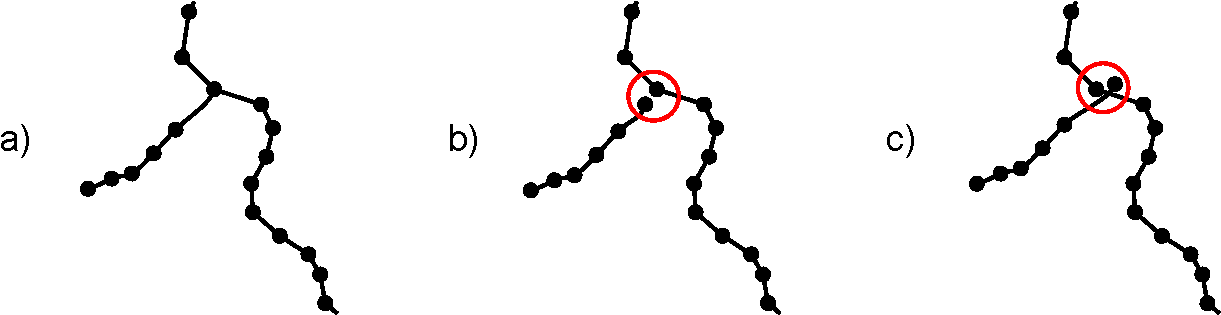
\includegraphics[width=\textwidth]{Data_sources/Imprecisiones_digitalizacion.pdf}
\caption{\small Errores derivados del proceso de digitalizaci�n. a) Versi�n correcta, con nodos coincidentes. b) y c) Versiones con errores que causan una falsa desconexi�n entre las l�neas.}
\label{Fig:Imprecisiones_digitalizacion} 
\end{figure}


Debido a esto, las capacidades de edici�n de los SIG incorporan funcionalidades que permiten evitar estos errores en el momento de la digitalizaci�n, ayudando al operario en su tarea y permiti�ndole alcanzar una exactitud y precisi�n imposible de lograr sin estas funcionalidades. Entre ellas, es especialmente importante el establecimiento de tolerancias y ajuste autom�tico en funci�n de ellas (esto se conoce con el t�rmino ingles \textbf{snapping}), que ayudan a garantizar la coincidencia entre los distintos v�rtices. 


El hecho de que exista una completa coincidencia es especialmente importante cuando la capa vectorial que se digitaliza contiene \textbf{informaci�n topol�gica}. La topolog�a exige que la coincidencia sea correcta y defina perfectamente la relaci�n entre las entidades. La digitalizaci�n de entidades, en caso de querer recoger su topolog�a, debe realizarse siguiendo reglas adicionales tales como la digitalizaci�n una �nica vez de los lados comunes de pol�gonos. Debe, asimismo, recoger informaci�n adicional, como por ejemplo la necesaria para la definici�n de nodos en los cruces entre l�neas cuando existe relaci�n entre estas.


\section{GPS}

Uno de los hitos en la aparici�n de nuevas fuentes de datos geogr�ficos es la aparici�n de los \textbf{Sistemas Globales de Navegaci�n por Sat�lite}. Se trata de sistemas que permiten \textbf{conocer en todo momento y en cualquier punto del globo la localizaci�n exacta de dicho punto} con un margen de error del orden de unos pocos metros o menos. Para ello, se basan en el env�o de se�ales entre un dispositivo situado en el punto concreto y una red de sat�lites, pudiendo establecerse la posici�n exacta mediante las caracter�sticas de dicha transmisi�n.

El ejemplo m�s extendido de estos sistemas es el \textbf{Sistema de Posicionamiento Global} (Global Positioning System, o \textbf{GPS}). El GPS cuenta con una constelacion de 24 sat�lites activos, as� como estaciones terrestres que los controlan, y su funcionamiento se basa en la \textbf{triangulaci�n de la posici�n} de una unidad receptora, mediante las se�ales procedentes de un cierto n�mero de sat�lites. Esta triangulaci�n se basa en distancias entre la unidad receptora y dichos satelites, las cuales se calculan mediante diversos mecanismos. La posici�n se calcula no �nicamente en sus coordenadas \emph{x} e \emph{y}, sino tambi�n en \emph{z}, es decir en elevaci�n. El sistema GPS emplea como sistema geod�sico de referencia el WGS84.


El dise�o de la red de sat�lites est� pensado para garantizar que en cualquier punto de la superficie terrestre y en cualquier momento, un receptor puede localizar el n�mero necesario de sat�lites para obtener con exactitud su precisi�n. 

Existen \textbf{numerosas fuentes de error} que causa desviaciones apreciables en el calculo de coordenadas mediante GPS. Entre ellas destacan los errores en la posici�n de los sat�lites, errores por el rebote de la se�al en otros con anterioridad a alcanzar el receptor, errores por el paso de la se�al por la atm�sfera, as� como los de precisi�n de los relojes empleados para el c�lculo de distancias. La \textbf{disponibilidad selectiva} era un error aleatorio introducido en la se�al GPS con fines militares, pero fue eliminada en el a�o 2000.

Entre las t�cnicas empleadas para corregir estas desviaciones, destaca el denominado \textbf{GPS diferencial}, pensado en origen para eliminar el error de la disponibilidad selectiva, aunque tambi�n eficaz para corregir una buena parte los restantes errores citados anteriormente.

Para la aplicaci�n del GPS diferencial se requiere no solo un receptor �nico (aquel del cual se quiere calcular su posici�n), sino tambi�n otro \textbf{receptor fijo} de referencia cuyas coordenadas se conocen con alta precisi�n. Este receptor fijo es, a su vez, un receptor de alta precisi�n y, adem�s de calcular su propia posici�n, emite informaci�n que las unidades receptoras pueden aprovechar para corregir sus mediciones. El receptor m�vil, l�gicamente, tiene que estar capacitado para este tipo de correcciones, para as� poder hacer uso de la se�al de la estaci�n de referencia.

El fundamento de esta t�cnica es que los errores que afectan al receptor m�vil \textbf{tambi�n afectan al de referencia}. No obstante, la magnitud del error que afecta al receptor de referencia puede conocerse, ya que se conoce la coordenada exacta de este, y en base a eso puede eliminarse el error que afecta al receptor m�vil, asumiendo que ambos errores son de similar �ndole.

En la actualidad, aplicando estas t�cnicas de correcci�n diferencial, un GPS puede obtener precisiones del orden de 2 metros en latitud y longitud, y 3 en altitud. Sin correcci�n diferencial, esta precisi�n es de unos 10--20 metros.

La precisi�n del sistema GPS depende del tipo de receptor GPS (o, en el lenguaje com�n, GPS a secas) que se emplee, obteni�ndose mayores precisiones con receptores m�s avanzados, siempre dentro de las posibilidades del propio sistema GPS. Existen muchas clases de receptores GPS, siendo dos de ellas las principales en relaci�n con los SIG:
\begin{itemize}
	\item \textbf{GPS para uso general}. Unidades \textbf{peque�as y port�tiles}, de bajo coste, para actividades al aire libre, donde no se requiere una precisi�n elevada sino simplemente un conocimiento de la posici�n aproximada. Se emplean, por ejemplo, para recoger rutas en senderismo o navegaci�n. 
	\item \textbf{GPS para la medici�n topogr�fica}. Unidades de medio tama�o, generalmente con una antena independiente que se conecta a la unidad y que el propio operario carga a la espalda. La antena garantiza \textbf{mayor precisi�n} y una mejor localizaci�n de sat�lites en condiciones tales como zonas bajo arbolado. Est�n pensados para un uso profesional en levantamientos o replanteos, ofreciendo buena precisi�n en todas las coordenadas. 
	
\end{itemize}	


La capacidad principal de una unidad GPS en relaci�n con un SIG es la de \textbf{recoger coordenadas}. Esta funcionalidad permite almacenar puntos o trazados completos, encontr�ndose el operario inm�vil o bien en movimiento a lo largo de dicho trazado. Es habitual utilizar los vocablos ingleses de la terminolog�a GPS para denotar los distintos elementos que pueden recogerse, conoci�ndose a un punto de inter�s aislado como \textbf{waypoint} y un trazado como \textbf{track}. Una serie ordenada de \emph{waypoints} se conoce como \textbf{route} (ruta).

En el trabajo con el receptor GPS, el operario se puede detener en un punto cualquiera y memorizar las coordenadas del mismo, a�adiendo as� un \emph{waypoint} a la lista de los ya almacenados. Para crear un trazado, se suele disponer de funcionalidades de recogida autom�tica de puntos, de tal modo que el receptor memoriza estos a intervalos fijos de tiempo. El operario simplemente ha de desplazarse por el trazado y dejar que el receptor haga su trabajo mientras tanto. 


\section{Informaci�n Geogr�fica Voluntaria}

Hemos mencionado ya que los dispositivos tales como receptores GPS de bajo coste pueden emplearse para recoger informaci�n geogr�fica y crear datos geogr�ficos, y que cuando esto se une a los conceptos participativos de la denominada \textbf{Web 2.0}, surgen iniciativas de gran inter�s en las que el usuario de a pie, sin necesidad de una formaci�n espec�fica como cart�grafo, puede aportar sus datos para que otros los exploten posteriormente. Aunque no se trata de una fuente de datos como tal, y los elementos y dispositivos empleados ya los hemos visto a lo largo de este cap�tulo, el cambio que supone la inclusi�n de una filosof�a acorde con las ideas de la Web 2.0 es tan notable que merece ser tratado por separado. No se trata de un cambio en la propia toma o preparaci�n de datos, o de una tecnolog�a nueva que se aplique a estos, sino de un \textbf{cambio social y filos�fico} que redefine el propio concepto de la informaci�n geogr�fica en lo que a la creaci�n del dato geogr�fico respecta, y cuyas consecuencias son ciertamente importantes, ya que abren el �mbito de la creaci�n cartogr�fica a un nuevo y amplio grupo de personas.

Se conoce como \emph{Informaci�n Geogr�fica Voluntaria o Participativa} (en ingl�s, Volunteered Geographical Information, VGI) al uso de Internet para crear, gestionar y difundir informaci�n geogr�fica aportada voluntariamente por usuarios de la propia red. El conjunto de herramientas y t�cnicas que emplean esos usuarios para aportar su informaci�n conforma lo que se ha dado en llamar \textbf{neogeograf�a}. La comparaci�n entre proyectos de creaci�n de VGI y la bien conocida Wikipedia sirve perfectamente para ilustrar qu� es lo que entendemos por VGI y neogeograf�a, ya que la VGI es el resultado de aplicar los conceptos de la Web 2.0 al �mbito de la informaci�n geogr�fica. 

En el caso particular de esta �ltima, la neogeograf�a ha supuesto un profundo cambio en algunas de las ideas b�sicas de la cartograf�a, modificando asimismo la concepci�n tradicional de la informaci�n geogr�fica, sus caracter�sticas o el papel que esta ven�a desempe�ando en muchos �mbitos (o incluso d�ndole un papel en campos donde con anterioridad el uso de informaci�n geogr�fica era escaso). Algunas de las ideas principales sobre la neogeograf�a son las siguientes:

\begin{itemize}
	\item \textbf{Popularizaci�n y democratizaci�n}. La producci�n cartogr�fica ha estado siempre en manos de gobiernos u organismos, y en muchas ocasiones fuertemente censurada debido a su elevado valor estrat�gico. Con la VGI, la creaci�n de informaci�n geogr�fica se democratiza y se convierte en un proceso participativo libre y sin restricciones.  Se invierte el esquema <<hacia abajo>> de producci�n y uso de informaci�n geogr�fica.
	\item Los ciudadanos se convierten en \textbf{sensores} y tienen mayor consciencia de su realidad geo--espacial.
	\item Se elimina parte del <<misticismo>> de la producci�n de informaci�n geogr�fica	
\end{itemize}

En la actualidad, el proyecto de VGI de mayor relevancia es \textbf{OpenStreetMap} (OSM), un <<proyecto colaborativo para crear mapas libres y editables>>.


\section{Metadatos}

Con independencia de la forma en que se hayan obtenido, los datos pueden requerir otros datos adicionales para interpretarse. Por ejemplo, si tenemos las coordenadas de un punto, para interpretarlo correctamente necesitamos conocer, entre otras cosas, el sistema de coordenadas en que vienen expresadas esas coordenadas. El dato con el que trabajamos (las coordenadas), requiere unos datos adicionales (por ejemplo, el c�digo EPSG del sistema de referencia empleado) para cobrar verdadero sentido.

Surge as� el concepto de \textbf{metadatos}. Los metadatos son \textbf{datos acerca de los datos}, y su misi�n es \textbf{explicar el significado de los datos}. Es decir, ayudan a los usuarios de los datos a entender mejor el significado que estos tienen y la informaci�n que guardan. Los metadatos son un documento adicional que acompa�a a los datos, y que permite una mejor gesti�n y una utilizaci�n m�s precisa de ellos.

Trabajando en el entorno de un SIG, los metadatos se \textbf{asocian a una capa y a su contenido}, y pueden \textbf{referirse a ambas componentes} (tem�tica y espacial)


El concepto de metadato no es algo nuevo y exclusivo de los datos digitales, ya que un mapa impreso tambi�n contiene metadatos en cierta forma. Una leyenda o un texto en un margen del mapa con informaci�n sobre la fecha en que se ha creado son tambi�n metadatos. En el caso de los datos geogr�ficos digitales, los metadatos no forman parte del dato directamente sino que \textbf{son independientes de este}. Ello permitir� \textbf{realizar operaciones separadamente con los metadatos}, tales como b�squedas, que abren nuevas posibilidades y dan un gran valor a estos.

Dos de las funciones principales de los metadatos son \textbf{garantizar el uso correcto de los datos y facilitar su gesti�n, localizaci�n y consulta}.

Los datos espaciales, como muchos otros datos, son creados habitualmente para un determinado objetivo, y este objetivo no ha de ser necesariamente evidente o contenerse como tal en los datos mismos. Cuando se emplean esos datos para un objetivo distinto a aquel para el que fueron dise�ados, pueden surgir problemas debido a que se est� realizando un proceso para el que los datos con los que se trabaja presentan carencias.  Por ejemplo, consultar los metadatos puede \textbf{evitar el trabajo con datos desfasados o de precisi�n insuficiente}, ya que conociendo estos par�metros es posible juzgar si los datos son adecuados al fin que se persigue con ellos.

Los creadores de datos deben procurar \textbf{acompa�arlos de metadatos precisos y suficientes}, y los usuarios deben \textbf{consultarlos antes de utilizar} dichos datos. 

Respecto a la gestion de los datos, los metadatos facilitan la organizaci�n y la realizaci�n de tareas tales como la busqueda de datos dentro de una colecci�n de estos. Los metadatos constituyen un <<resumen>> de las caracter�sticas principales de los datos, y pueden ser empleados para labores de b�squeda y localizaci�n de datos de un tipo dado. Los metadatos \textbf{facilitan y agilizan la localizaci�n} de los datos cuando estos se buscan \textbf{por criterios geogr�ficos}. A�adiendo a los metadatos elementos como la extensi�n del �rea cubierta por los datos, este tipo de b�squedas se efect�an de forma m�s �gil y efectiva. En este sentido, el uso de metadatos es fundamental para el establecimiento de \textbf{catalogos de datos}, los cuales ya que responden a las peticiones del usuario del cat�logo en funci�n de la informaci�n que los metadatos contienen.


\subsection{Contenido y creaci�n de metadatos}

La informaci�n que contienen los metadatos para una capa de datos espaciales depende de factores tales como el \textbf{modelo de representaci�n} empleado, el \textbf{formato} en que se almacenan los datos (formato de archivo, base de datos, etc.), la \textbf{organizaci�n, entidad o individuo responsable} o el \textbf{elemento al que se asocian} (conjunto de capas, capa individual, entidad\ldots).
 
 
Algunos de los elementos comunes que se incorporan a los metadatos geogr�ficos son la informaci�n \textbf{de identificaci�n} (para identificarlo de forma �nica y distinguirlo de otros), la informaci�n \textbf{sobre la calidad de los datos} (incluyendo su origen y el de los datos de los que deriva, apareciendo asi el concepto de \textbf{linaje} de los datos), la informaci�n \textbf{sobre la componente no espacial} o la informaci�n \textbf{sobre la distribuci�n} (acceso, licencias, etc.)

Los metadatos puede \textbf{crearse en el origen} mismo de los datos, recogiendo la informaci�n al mismo tiempo que se producen los datos en s�. Tambien pueden \textbf{extenderse posteriormente} por parte de distribuidores, organizadores o usuarios.

La creaci�n de los metadatos se realiza en su mayor parte \textbf{de forma manual}, existiendo aplicaciones espec�ficas para ello. Los metadatos que pueden extraerse de las capas de datos directamente, tales como la extension cubierta por estos, pueden crearse de forma autom�tica.

Los metadatos se almacenan en general como \textbf{ficheros adicionales} a los ficheros de datos, o bien como \textbf{parte de una base de datos}.




\pagestyle{empty}


\chapter{Software and technology}

\pagestyle{fancy}

The classic concept of GIS is that of a complete software application which implements all the tools needed for working with geographical data: creating or editing, managing, analyzing and visualizing. Along with that, other types of applications have appeared which, although they do not match exactly that definition, have to be considered as part of the GIS world.

We will divide GIS applications into three main blocks: \textbf{desktop GIS, web-based GIS}, and \textbf{mobile GIS}. They will be described in detail in this chapter. We will also provide additional information about some technologies that they are based on.


\section{Desktop GIS}

There are five fundamental functionalities of a desktop GIS: \textbf{data input and output, visualization, editing, analysis, and map design}. Most desktop GIS tools have these five capabilities, although the level of functionality for each of them might differ. Some tools might be more prepared for data editing, while others might focus on analysis.

\subsection{Data input and output}

A desktop GIS must be able to \textbf{read data} and, optionally, to \textbf{save} it. This last functionality is needed in case the GIS can produce new layers, but not in those that do not contain analysis or editing capabilities.

There are a \textbf{very large number of data formats for geographical data}, and most GIS use common libraries to be able to read and write them, allowing them to share data among them and improve their connectivity.

Apart from being able to read data files, it is now also important to be able to connect to \emph{databases} and \textbf{remote services}. We will talk about those later in this chapter.

\subsection{Visualization}

Visualization is a fundamental capability of GIS. It is, of course, important when the main purpose of using GIS is to create cartography, but also when our work is focused on data editing or analysis, since visual exploration of the data is a previous step.

The visualization part of GIS is mainly comprised of a \textbf{canvas} on which layers are rendered. The user can add or remove layers, and also change their \textbf{symbology}, that is, the way in which the layer data is converted into graphical elements. Layers are rendered in a given order which allows to create a \emph{rendering hierarchy}.

Along with the canvas, there are \textbf{navigation tools} that allow the user to modify the area that is being displayed by zooming in, zooming out or panning (Figure \ref{Fig:Navigation_tools}). 

\begin{figure}[!hbt]
\centering
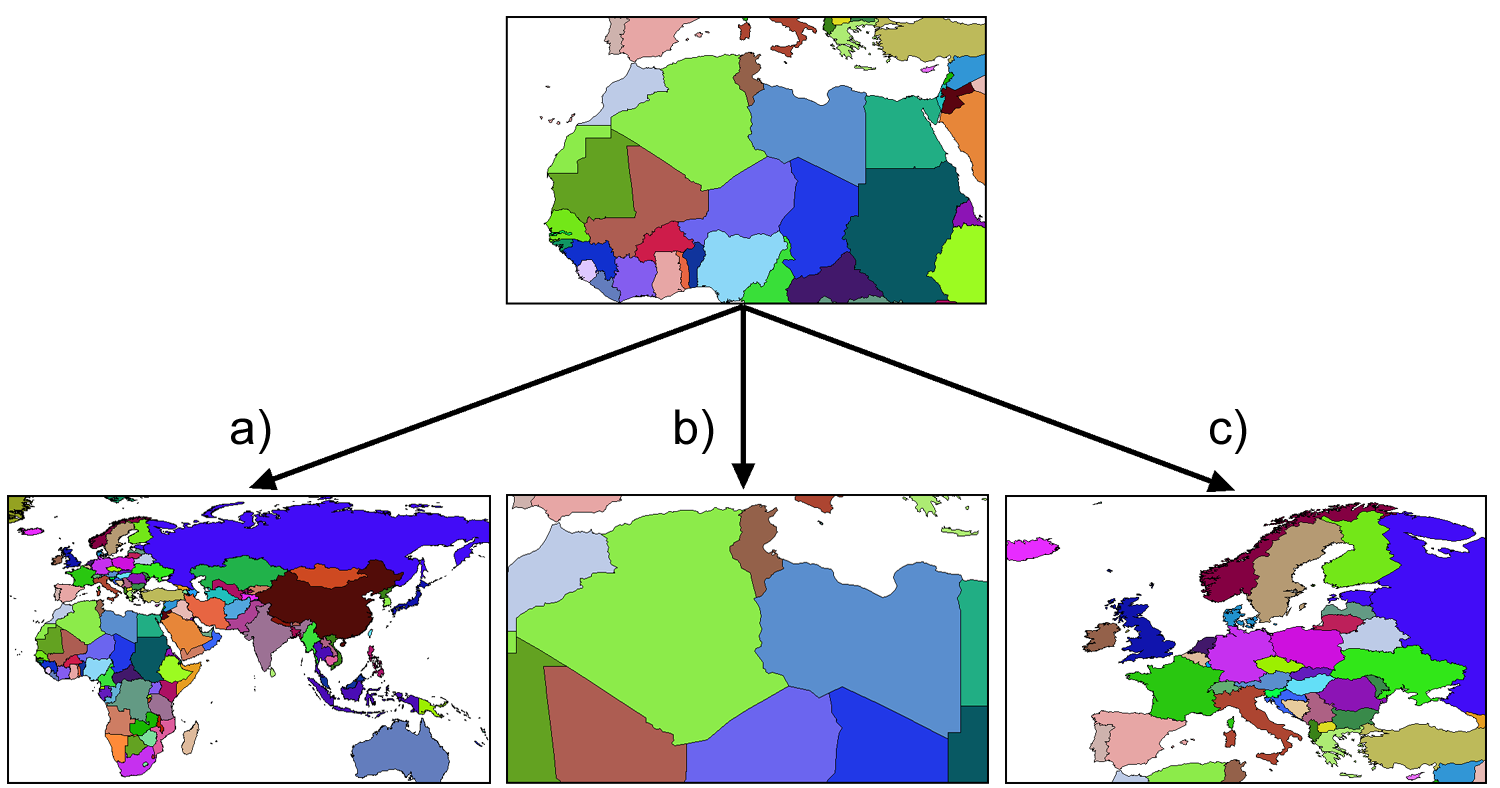
\includegraphics[width=.99\textwidth]{Software/Navigation_tools.png}

\caption{\small Navigation tools that are common in a desktop GIS. a) zoom out, b) zoom in, and c) pan}
\label{Fig:Navigation_tools} 
\end{figure}

The most remarkable feature of geographical data visualization in GIS is that, unlike what happens with a classic printed map where its characteristics cannot be changed, the user can select \emph{what} he/she sees and \emph{how} he/she sees it. Geographical data is \textbf{independent of the information needed to visualize it} and, therefore, it can be represented in different ways. This is true even for data that has an inherent visual nature, such as images, since even in that case the rendering can be adjusted and modified by the user.

Although in the most common case the canvas is bidimensional, certain GIS are also capable of \textbf{three-dimensional rendering}. In this case, navigation tools are more complex and they allow for adjusting perspective, vision angles or vertical exaggeration, among other parameters.

\subsection{Analysis}

Analysis is a fundamental functionality of GIS since its origins. Others, such as visualization, although we cannot imagine GIS without them nowadays, were very limited in the early days. Analysis, however, has always been at the core of GIS.

The current trend in GIS is to consider analysis capabilities as \textbf{modular tools} that are run on a base platform which includes the data input and output capabilities, along with the visualization component. Analysis tools are independent, but they can be used together to create more complex analyses.

Analysis tools might be completely independent of the visualization component or be linked to it. In the first case, the analysis is performed on a set of layers and parameters without any interaction with the map while in the second case, the user might interact with the view to define how the analysis is performed (for instance, selecting a coordinate or a region in the canvas which will then be used as a parameter for the analysis tool).

The result of an analysis tool in GIS can be geographical (a new layer) or not (a simple value, such as the one resulting from some statistical analysis of the input data).

Analysis tools can be organized into \textbf{workflows} which help\textbf{automate} analysis routines. Also, the analysis functionality of desktop GIS can usually be used from \emph{scripting languages}, which allow definition of more complex models and data flows. This is one of the main strengths of current GIS tools, since it provides the user more power and flexibility.

\subsection{Editing}

The geographical data with which we work in GIS are not static. Information contained in a layer \textbf{might have to be changed or corrected}, and the functionality that allows the user to do that is important if we want the GIS tool to be versatile. Without them, geographical data lose part of their potential, and that is the reason why most desktop GIS tools implement editing capabilities to some extent.

This capabilities can be used to \textbf{create new layers} or to \textbf{update existing ones}. The following are some editing tasks that can be performed with GIS:

\begin{itemize}
\item Editing the geometries of a vector layer feature.
\item Editing the attribute values of a vector layer feature, including editing the list of attributes of the layer, adding or removing them.
\item Adding new features to a vector layer or removing existing ones.
\item Editing cell values in a raster layer.
\end{itemize}

Tools used to edit geometries inherit a large part of their design from CAD software. In certain cases, they are extended with new functionalities, as happens in the case of editing geographical data with topology (CAD software does not consider topology).


\subsection{Map design}

Most desktop GIS are capable of producing cartographic documents which can later be printed and used as a classic paper map. These documents are composed in the GIS from the data, and use the same functionality that it is used for the on-screen rendering (symbology, etc.).

Along with that, other tools allow the user to \textbf{design and compose the map}, and to \emph{adjust its elements} (rendered layers, legend, title, etc.), and are inspired by those found in design software. 

Some desktop GIS include elements to \emph{automate cartographic production}, such as templates or tools to generate map series (Figure \ref{Fig:Map_series}).

\begin{figure}[!hbt]
\centering
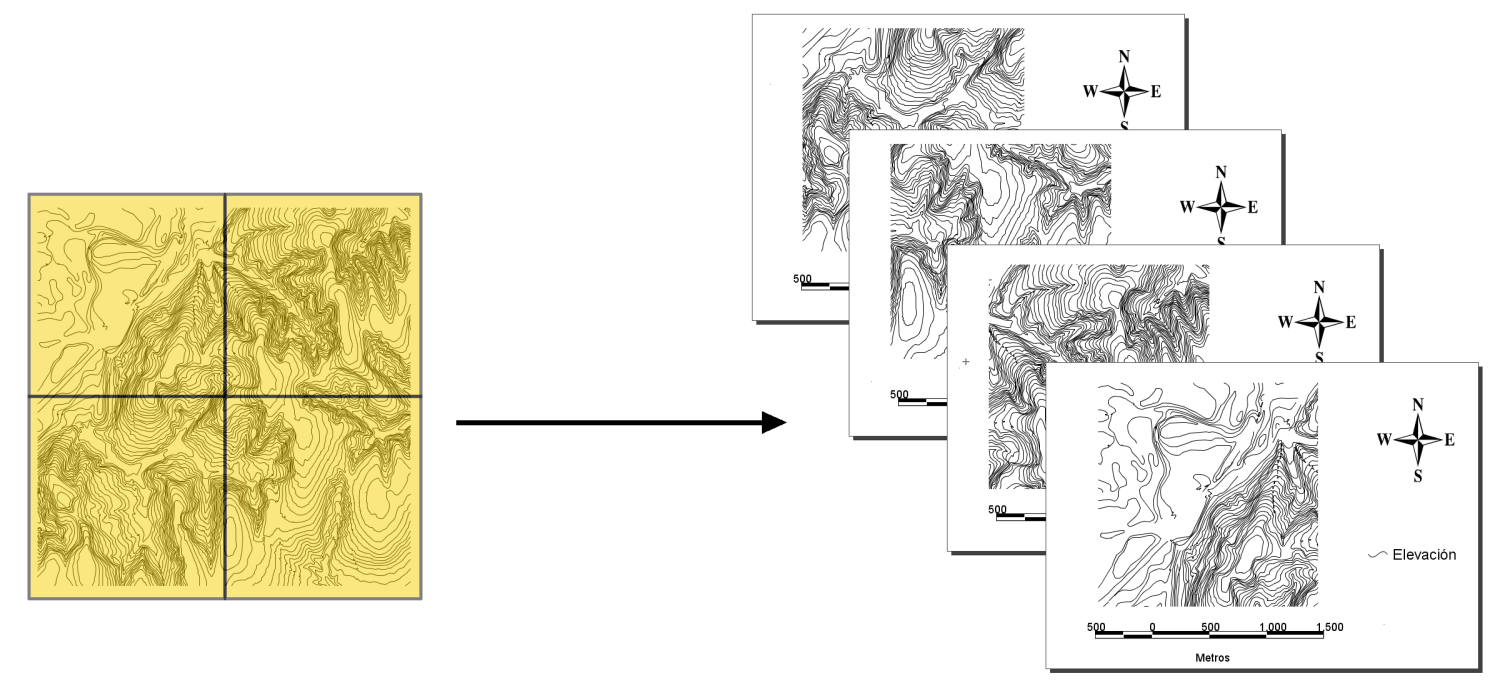
\includegraphics[width=\textwidth]{Software/Map_series.png}
\caption{\small Automated creation of map series in a GIS.}
\label{Fig:Map_series} 
\end{figure}

This is possible thanks to the \textbf{separation between geographical data and the design of the cartographic document}, similar to what we noted for the case of visualization.


\section{Web mapping. Clients and servers}

One of the most relevant advances in the history of GIS is the advent of \textbf{Web mapping}. Web mapping technologies are used to incorporate GIS elements as part of websites, with internet browsers being then the base platform on which GIS functionality is executed. These technologies include not just the elements run on the browser, and have been key in shaping and developing others such as \textbf{remote data services}, which are used not only by Web Mapping applications but also by desktop GIS.

The concepts of \emph{server} and \emph{client} are fundamental in this context. Let's discuss them in a bit more detail.

A \textbf{server} is the element that provides (serves) a given content through the network. In our GIS context, this content means basically geographical data. The \textbf{client} is the element that requests the data, receives it and works with it. 

A web browser is a client, since it makes a request to get the content of a website and shows it to the user. When we enter a web address in the address bar of a web browser, we provide the information needed to establish the connection between the server and the client and to transfer the data from one to the other.

Let's see how that works. Suppose that we want to visit the following website:

\begin{center}
\small\texttt{http://victorolaya.com/writing}
\end{center}

The requests is done based on the web address ---more technically, a Uniform Resource Locator (URL)---, which is a reference to a web resource that specifies its location on a computer network and a mechanism for retrieving it. We can divide it in the following parts:

\begin{itemize}
	\item \texttt{http}: The protocol to use, which defines the way client and server will communicate with each other.
	\item \texttt{victorolaya.com}: The host name. This part identifies the server machine connected to the network where the page that we want to visit is stored. It is a human-readable version of a numeric code that indicates the address.
	\item \texttt{writing}: The page we want among all the ones that the server can provide. 
\end{itemize}

The process that allows us to have that page in our web browser comprises the following steps:

\begin{enumerate}
	\item The client makes the request.
	\item The server machine is identified and the request is driven to it.
	\item The server prepares the page that has been requested and sends it back to the client (or it sends an error message in case it could not find or prepare the page).
	\item The client receives the page and renders it so the client can see it.
\end{enumerate}


Figure \ref{Fig:How_internet_works} shows a summary of this.

\begin{figure}[!hbt]   
\centering
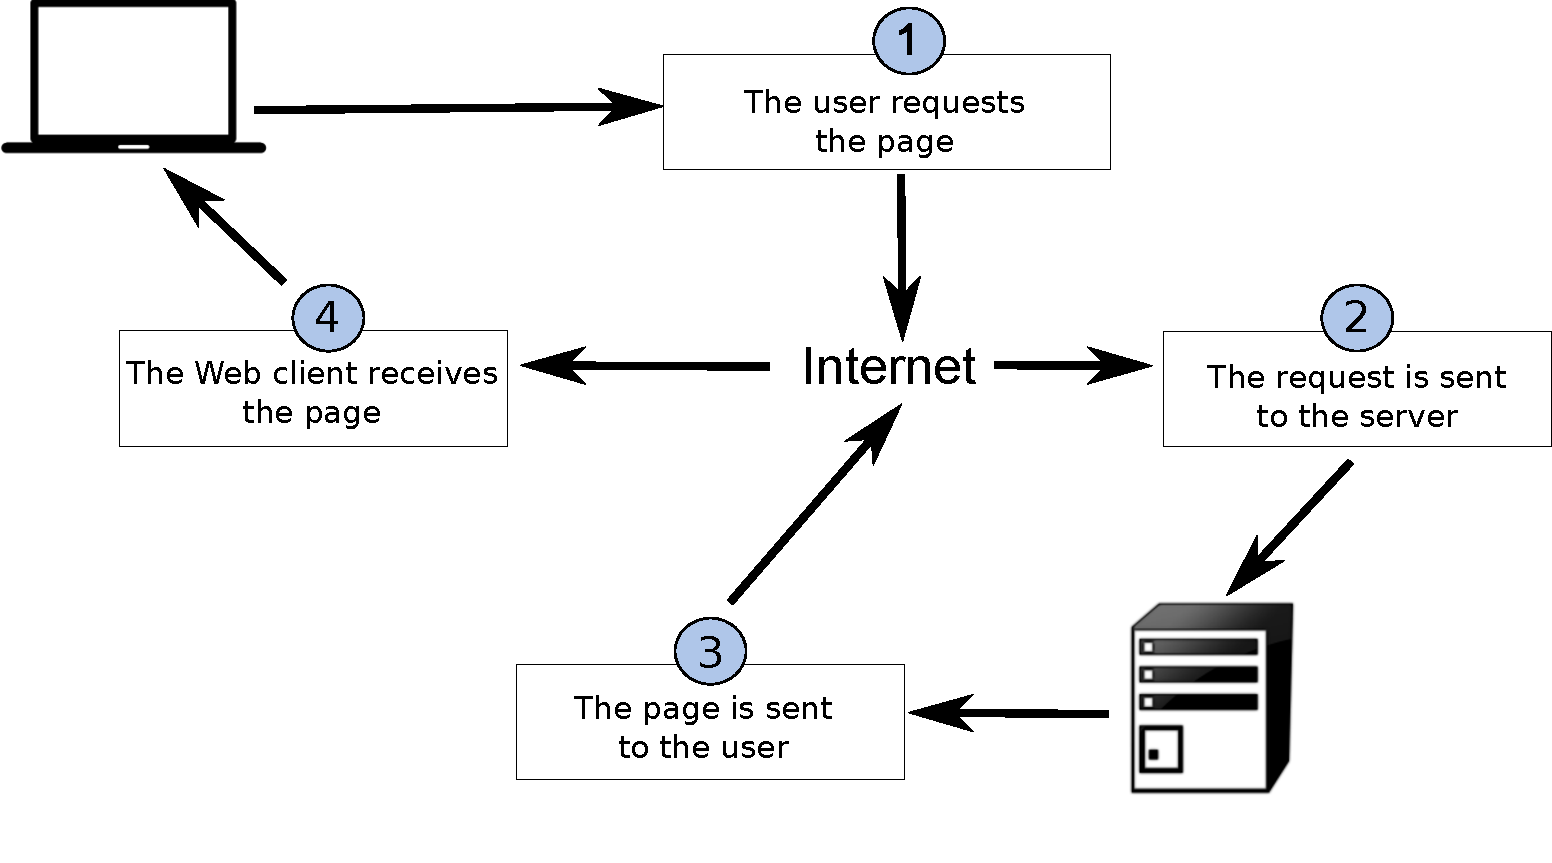
\includegraphics[width=\columnwidth]{Software/How_internet_works.pdf}
\caption{\small Client-server interaction mechanism that takes place when visiting a website.}
\label{Fig:How_internet_works} 
\end{figure}

A relation is established between clients and servers, in which an arbitrary number of clients connect themselves to a server, from which they obtain data whenever each of them makes a request. In this client-server architecture, the server has the data to be shared through a service, while clients only provide information about themselves needed to validate and perform the data sharing.

Now let's see how these ideas apply to the field of GIS.

Regarding servers, they can have four main capabilities:

\begin{itemize}
\item \textbf{Serve rendered geographical data}. Generally known as \textbf{map servers}, they provide maps. That is, images created from geographical data. If data is already an image (such as an aerial or satellite photograph), the server will just send it as it is. If data is not an image (vector layer or raster layer other than image), the server will create an image based on the geographical data. The symbology used to do this can be a default one that the server uses for all requests or it can be provided by the client in the request. 

In both cases, the client also specifies the dimensions of the requested map image that is served, and then the server prepares it.


\item \textbf{Serve the data directly}. A more flexible option is to serve the geographical data itself. The client requests the data and once it has been transmitted across the network, can use it however he/she needs. In case the data is to be visualized, the symbology has to be set in the client side, since the server is not taking care of that and provides the raw data.


\item \textbf{Serve the result of queries}. Another functionality that the server can have is to return not just the full set of geographical data, but a subset of it. The client can specify a \textbf{filter} and the server will use it to create a subset that will later be sent in the response. Also, the server can provide \textbf{descriptive values} about the data it has. The client, which might be connected to several services and obtain the values, can use those values to filter which services to use (for instance, asking them the extent of their data and then selecting only those that have data about a given study area). As we have already seen, \textbf{metadata} have a great relevance in this context, since they allow this kind of queries to be executed (and the corresponding requests to be responded to) efficiently.

\item \textbf{Serve processes}. Finally, a server can provide new data, whether geographical or not, computed from geographical data. In this case, the server provides a processing service, and it processes the data that is passed to it as part of the request. The request can contain the data itself, or a reference to it. If a reference is passed, the data might already be in the server, or it can be in another one. In this last case, the first server will become a client of the second one, will retrieve its data, process it, and send back the result to the original client (Figure \ref{Fig:Remote_data_and_services}).


\begin{figure}[!hbt]   
\centering

\includegraphics[width=0.95\textwidth]{Software/Remote_data_and_services.png}
\caption{\small Remote processing service using data from a second server.}
\label{Fig:Remote_data_and_services} 
\end{figure}

\end{itemize}

About clients, they can be divided in two classes:

\begin{itemize}

	\item \textbf{Heavy clients}. Heavy clients are independent applications that do not run on top of another one such as a web browser. They usually have a larger size since the application has to care of all the program logic.

	Heavy clients handle and use data not coming from web services, such as local data files. They are not just clients, but full-fledged applications that work even without its client part.

	Nowadays, most desktop GIS are heavy clients themselves as they have the functionality of classic GIS but can also consume web services.


	\item \textbf{Light clients}. They normally have a smaller size and their capabilities are more limited. They run on web browsers and most of the time rely on remote data from servers.

	Although originally, they focused on data visualization (adding map views to websites, with a certain degree of interactivity), they have begun to implement more advanced functionalities such as analysis functionality (whether on the client side or using a processing service) or data editing.

	The term \emph{Web mapping} is used to refer to the lighter clients which focus only on rendering maps, while the term \emph{Web GIS} is used for those with more functionality, incorporating some of the tools traditionally found in desktop GIS.
\end{itemize}

\section{Some techniques related to GIS services}

Two important techniques used in the context of the client--server architecture for geographical data are \textbf{tiling} and \textbf{caching}. These techniques, whether implemented on a light client or a heavy one, allow for more responsive interfaces and reducing the amount of data sent over the network, overcoming to a certain extent the problems that a slow network might cause. Both are used mainly with map servers (servers that provide rendered images).

Tiling divides the images that the client is working with into smaller ones, forming a mosaic. By correctly managing the tiles in that mosaic, the amount of data transmitted can be reduced. When the request is sent to the server, instead of a single image, a set of them is requested. Although this does not reduce the amount of data, the tiled structure will allow a more flexible and optimized handling of data once a new image is needed, as will soon be explained.

Caching is a technique frequently used not just for web SIG, but as a general tool in the context of the internet. Web browsers store previous responses from web servers, such as web pages and images, in a so-called \emph{cache}. When data that was previously requested is requested again, it can be taken from the cache instead of from the corresponding server, which is usually faster and more efficient.

Combining tiling and caching increasing responsiveness and results in an optimized data management. Let's see how that works, using the example shown in figure \ref{Fig:Tiling}.

\begin{figure}[!hbt]   
\centering
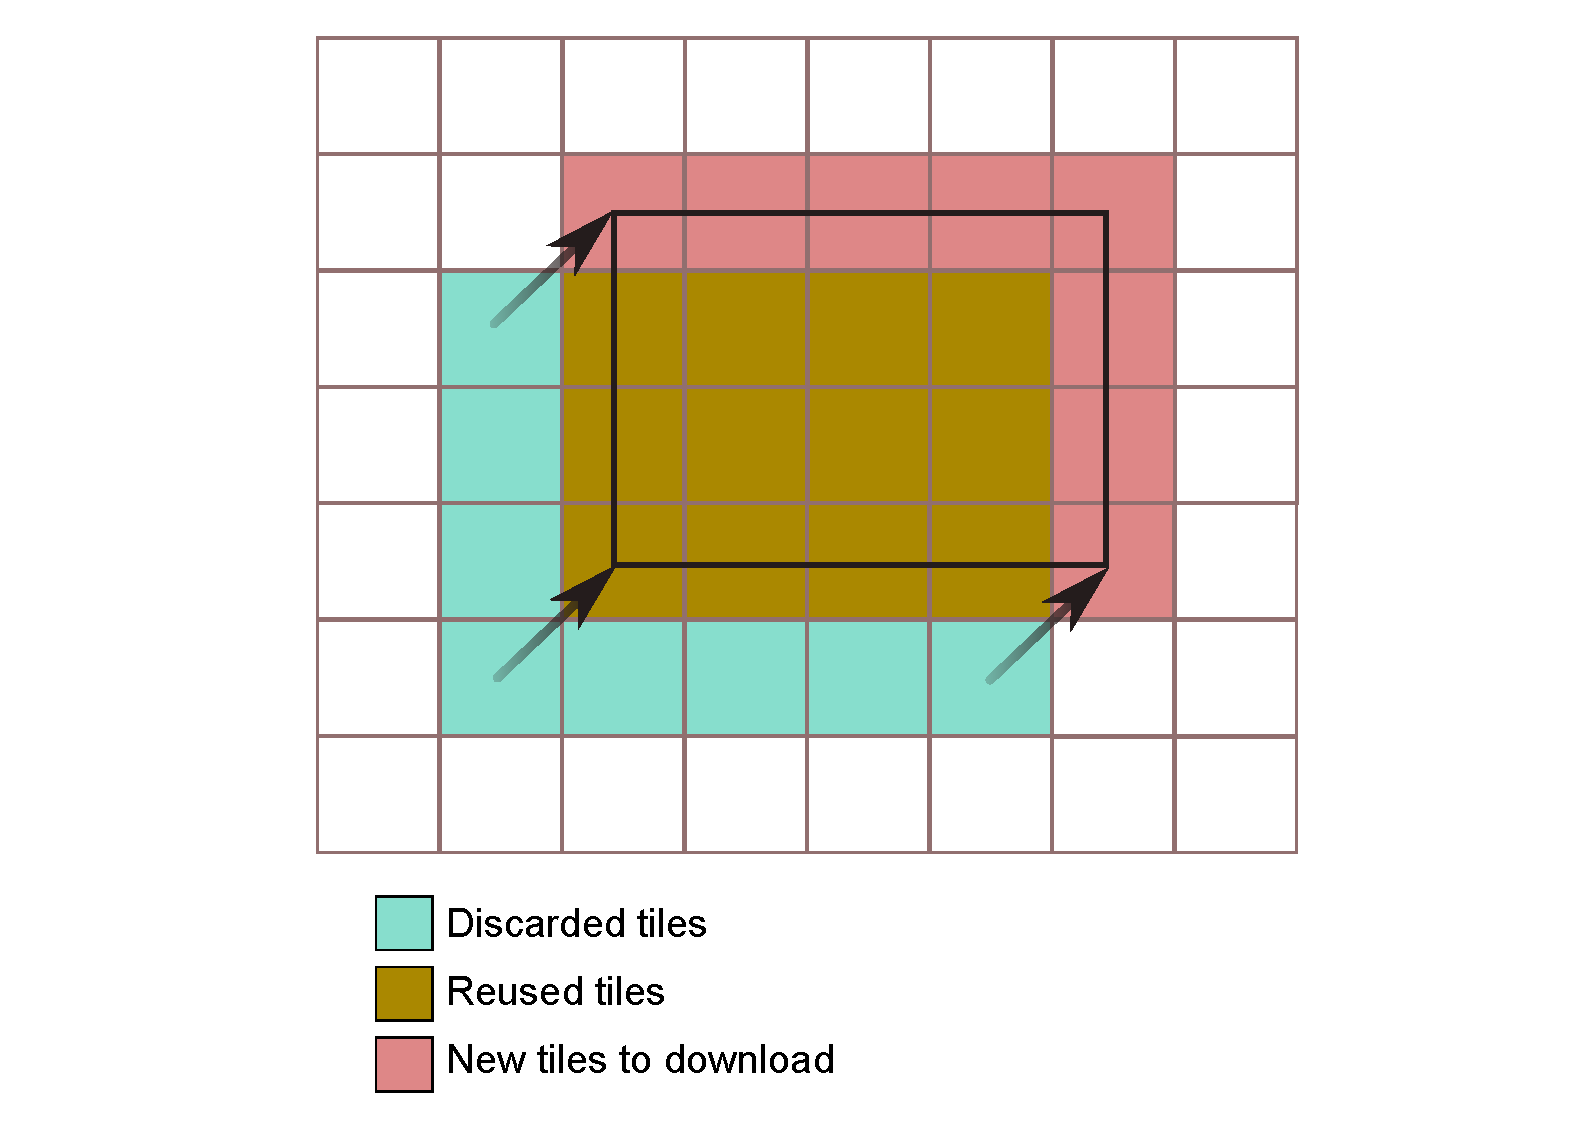
\includegraphics[width=\textwidth]{Software/Tiling.pdf}
\caption{\small Combination of tiling and caching techniques to optimize data handling in a web GIS application.}
\label{Fig:Tiling} 
\end{figure}

Initially, the application displays an area that cover 20 elements or tiles. All those tiles have already been downloaded from the server, and stored in the application cache, which means that using them again does not require making a new request to the server. Without caching and tiling, when the application user changes the area to be displayed as shown in the figure, a whole image has to be requested, with exactly the same size as the image to be rendered in the screen. However, if tiling and caching are applied, we just have the whole new image to be painted divided in 20 parts, and, since some of them are stored from a previous request, we just have to request a small number of them (8 in this case, corresponding to the areas not covered by the previous image). The amount of data that is requested to the server and transmitted over the network is much smaller.

Caching can also be implemented on the server side. We have seen that map servers provide already rendered images based on some data. Rendering that data can be time consuming and, if it has to be done for each request, that would mean a lot of computing cost for the server. Instead, images are pre-rendered at different scales so when a client request is received by the server, it just has to crop the pre-rendered image instead of producing the response image from the base data.

A recent technique that is gaining popularity is \emph{vector tiling}. Using the same approach as in the case of the tiling we have just seen (that is, cutting the data in pieces), vector layers are divided and only the required data are sent to the client.

This allows the client to request and use vector layers and be responsive at the same time. Without vector tiling, this would be impossible for large layers. The advantage in this case is that the symbology can be defined by the client. Also, the user experience is improved, since for instance, transitions become more fluent when changing the map scale, due to the scalability of vector data.




\section{Standards}

To ensure the the client-server system works correctly, it is important to define how the communication between servers and clients takes place. Some \textbf{normalization} is needed, and there must be common and well-defined elements implemented by both the client and the server. This \emph{lingua franca} that allows clients and servers to communicate is what we call a \textbf{standard}.

In an ideal situation, a complete \textbf{interoperability} would exist independent of formats and applications used. Clients and servers would be able to connect with each other, regardless of their own characteristics. Standards are the element that allows that to happen, because they define a common framework in which clients and servers communicate. As long as a client or a server follows the standard, it will be able to communicate with all others that do it as well. Standards provide \textbf{technological homogeneity}.


Interoperability means that any element of the client-server system can be replaced with another one, and the interaction between all parts of the system will not  be affected. A client or server might have different functionalities, but regardless of its origin (its manufacturer), it will be able to interact with the other elements, if all implement the same standard.

A standard is considered as such when it is used by a group or community, which accepts it to define the characteristics of a product or service within it. Standards can be established by public acceptance and custom (\emph{de facto} standards) or they might have legal recognition and be proposed by some official organization (\emph{de iure} standards).

A standard is \textbf{open} if \textbf{its definition is available} to everyone who wants to know more about it and use it for any activity related to it.

The following are some of the fundamental principles that open standards are based on:

\begin{itemize}
	\item \textbf{Availability}. Open standards are available to anyone, to read and to use.
	\item \textbf{Maximize end-user choice}. Open standards create a fair, competitive market, and do not lock users in the closed environment of a given vendor. 
	\item \textbf{No royalty}. Implementing a standard is free and has no cost, unlike the case of a patent.
	\item \textbf{No discrimination}. Open standards and the organizations behind them do not favor any implementer of the standard over the rest of them.
	\item \textbf{Extension or creation of subsets}. Standards can be extended with additional elements or reduced to less-detailed subsets.
\end{itemize}

To know the impact that a standard has in the context of GIS, let's take a look at figure \ref{Fig:Non_interoperable}, which represents a non-interoperable architecture that does not use standards.

\begin{figure}[!hbt]   
\centering
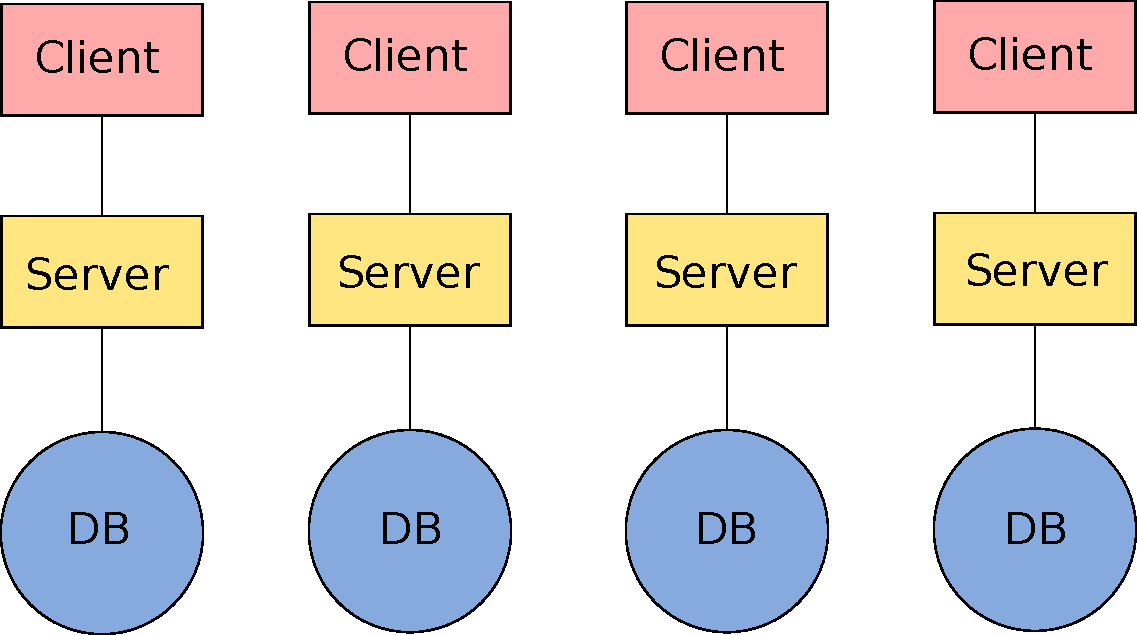
\includegraphics[width=.7\columnwidth]{Software/Non_interoperable.pdf}
\caption{\small Non-interoperable architecture.}
\label{Fig:Non_interoperable} 
\end{figure}

Data stored in each database are available only by using one client, the one corresponding to the server that serves those data. The remaining data are not available for that client. Each client-server-database group is an independent island, technologically isolated from the rest of them.

Disadvantages of a non-interoperable architecture like that include the following:

\begin{itemize}
\item \textbf{Waste of resources}. Each service must manage its own data. That is complex and has higher costs than sharing data with other compatible services.
\item \textbf{Need to know multiple clients}. Since we need a different client for each service, the user must be familiar with all of them. Being capable of using just one client is not enough to use all the available data, since that client can only access a small part of all that data..
\item \textbf{Combining data is not possible}. Two datasets that are available through two different services cannot be used in the same client, as it cannot communicate with the corresponding servers.
\item \textbf{Combining functionalities is not possible}. If data is only available to a given client, the functionality in another one (which might not be implemented in the first) cannot be used on that data. When working with that data, the user's possibilities are limited to what the corresponding client can do.
\end{itemize}

Now let's take a look at a fully interoperable architecture based on open standards, as seen in figure \ref{Fig:Interoperable}.

\begin{figure}[!hbt]   
\centering
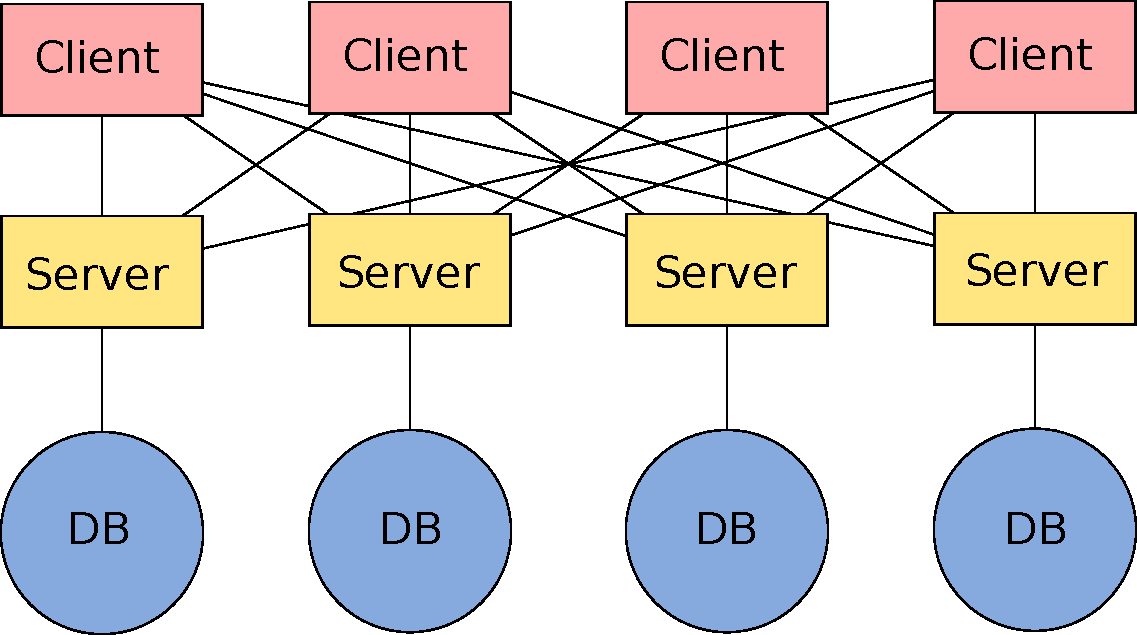
\includegraphics[width=.7\columnwidth]{Software/Interoperable.pdf}
\caption{\small Interoperable architecture.}
\label{Fig:Interoperable} 
\end{figure}

In this case, there is a server that manages and offers the services for each database, but all clients can access all servers, since they are based on open standards and communication is possible between any two of them.

\subsection{Relevant standards in GIS}

The most common standards for geographical information are created and promoted by the  \textbf{Open Geospatial Consortium (OGC)}. The OGC is ``an international not for profit organization committed to making quality open standards for the global geospatial community''.

Some of the most relevant OGC standards are the following ones:

\begin{itemize}
\item \textbf{WMS}. To serve maps (images)
\item \textbf{WCS}. To serve coverages (currently only raster layers).
\item \textbf{WFS}. To serve geographical features and attributes (vector layers). It can also allow editing features from the client.
\item \textbf{WPS}. To serve remote processing services.
\item \textbf{GML}. To store geographical information.
\item \textbf{CSW}. To make queries to a catalog that contains geographical data.
\end{itemize}

Each one of these standards is described in the corresponding specification, which is subject to change and improvement. Several versions exist for each of them.

Along with these standards are those made by organizations such as \textbf{ISO} o \textbf{W3C}, with a more general scope, but also important in the context of GIS. Among them, the most relevant standards are the ISO ones that define \textbf{how to store metadata} and the W3C standards related to \textbf{communication over the Internet}.

\section{Mobile GIS}

GIS on mobile platforms such as mobile phones or tablets has a clear relation with both desktop GIS and web GIS. It takes the elements from them and adds others derived from running on a mobile platform which expand their possibilities.

Mobile devices nowadays offer two main capabilities from the point of view of GIS: \textbf{wireless access to Internet} and \textbf{ability to know the position} of the device. 

Internet access can be used to obtain maps and geographical information from a given server, or to send field data acquired with the aid of the mobile device.

The position of the mobile device is usually known based on the GPS receiver that is part of most mobile phones. However, other approaches are also possible, from computing the position \textbf{based on the phone network} to using some \textbf{indoor positioning system} if it is available.

Knowing the position of the device allows the mobile GIS application to provide additional functionality. For instance, it might be used to make \textbf{field data acquisition} easier and more efficient (the coordinates of measured points do not have to be entered manually), or to provide \textbf{location-based services} (LBS).  

Some of the main groups in which these services can be grouped are listed next.

\begin{itemize}
	\item \textbf{Navigation}. Shortest path computation, route guidance, etc.
\item \textbf{Data acquisition}. Any type of data can be registered in the field, and the device associates to them its own position automatically.
\item \textbf{Information}. Business directories, travel guides, etc.
\item \textbf{Advertising}. Location-based advertisements, promotions for nearby shops, etc.
\item \textbf{Tracking}. Of both people and products, along predefined routes or arbitrary ones.
\item \textbf{Management}. Of infrastructures, installations or fleets.
\end{itemize}

When running in a mobile platform, a GIS has additional information about the context it is running on (position, direction of movement, speed, illumination, etc.), that it can use to provide more functionality than a desktop or web GIS running on a non-mobile platform.

\pagestyle{empty}

\chapter{Databases}

\pagestyle{fancy}

Databases are used in all disciplines in which an efficient data handling is needed, specially if those data are large. The data that is used in GIS are usually rather large, and the improvements in data acquisition have caused geographical data to be now more precise and, consequently, larger. 

Databases not only have the advantage of being able to work with large datasets, but also other ones such as managing multiple users or providing efficient access and indexing. For this reasons, they are a fundamental element in any software context, including GIS.

A \textbf{database} is an \textbf{organized and systematically stored collection of data}. Databases provide a better way of handling and using data, thanks to their structure.

Some of the advantages of using a database instead of a traditional file-based approach for storing data are:

\begin{itemize}
	\item \textbf{More independence}. Data are independent from both the users and the software.
	\item \textbf{More availability}. Databases facilitate the access to data from different context and applications, making them more useful for a larger number of users.
	\item \textbf{More security (data protection)}. Replication and synchronization of data becomes easier.
	\item \textbf{Less redundancy}. Which implies a smaller volume of data and faster access.
	\item \textbf{More efficiency in data capture, encoding and input}.
\end{itemize}

This has a direct influence in the results that are obtained from the explotation of database data, and we find the following advantages:

\begin{itemize}
	\item \textbf{More coherence}. Better management leads to better data, and that produces results with a better quality.
	\item \textbf{More efficiency}. Accessing the data is easier and more effective.
	\item \textbf{More informative value}. It is easier to extract the information that is contained in the data, since one of the goals of a database is the increase the value of data as source of information.
\end{itemize}

Users also get advantages when using a database, such as the following ones:

\begin{itemize}
	\item \textbf{Easier access}. The user of the database just has to worry about \emph{using} the data. A solid infrastructure to do it is available, and so are the tools needed for it.
	\item \textbf{Easier data reutilization}. Data is easier to share when using a database.
\end{itemize}

In short, we can say that the main characteristic of a database is the \textbf{centralization} of data that it implies, which results in a \textbf{better data access, management and organization}.


\section{Relational databases}

From the many different models that have been defined for creating a database, the most popular one, both in the GIS context and outside of it, is the one used in databases known as \textbf{relational databases}. This model uses a scheme based on \textbf{tables}, which is both easy to understand and to use for analysis and data queries. Tales have a certain number of \textbf{records} (rows) and \textbf{fields} (columns).

The table itself is knows as a \textbf{relation}, since it contains the relation that exists between its elements. Columns represent the \textbf{attributes} associated to a feature, while rows contain the \textbf{records}. A row is formed with a set of $n$ attributes, which form a \textbf{tuple}.

A database usually contains more than a table, since the information to store is of many different types, and it is convenient to separate it into several tables. Apart from the relations that the table itself implies, relations between tables can also be defined. This is commonly know as a table \textbf{join}. To perform a table join, we need to have some attribute that can be used to unequivocally represent a tuple. This attribute is known as a \textbf{key attribute}, and it must be \textbf{unique and invariable} for each tuple. For instance, if we have a table where each row represents a person, an attribute containing the Social Security can be used as a key attribute.

When working with geographical data, it is common to use \textbf{the spatial component as key}, since it is usually unique.

Relations between tables can be of several types, depending on the records of one table that are related with the ones of the other table. We have \textbf{one to one}, \textbf{one to many} and \textbf{many to many} relations. for instance, if we have a table with cities and another one with persons, and we define a relation \emph{lives in}, it will be a one to many relation, since many people can live in a a single city, and each person lives in only one of them.


\section{Database management systems}

Along with databases, the fundamental element to exploit them are \textbf{database management systems} (DBMS). These systems are an \textbf{intermediary element between the data and the software that consumes them}. Software such as a desktop GIS does not access the database directly, but instead \textbf{through a DBMS}.

The following are some of the characteristics that a DBMS must have:

\begin{itemize}
	\item \textbf{Transparent access to data}. The DBMS creates an abstraction of the data that makes it easier to work with them, hiding the internal elements that are not relevant for exploiting the data.

	Procedures such as \textbf{queries} are done through a DBMS, which takes care of interpreting them, apply them on the database and returning the corresponding result. The GIS does not query the database, but instead communicates with the DBMS.
	\item \textbf{Data protection}. If the database contains sensible information, a DBMS must \textbf{control the access to it}, restricting it to certain users and implementing the protection mechanisms that are needed for this.
	\item \textbf{Efficiency}. A DBMS must be capable of efficiently handling \textbf{a large volume of data and a large number of operations} (for instance, many users accessing simultaneously), and provide a quick response to user requests.
	\item \textbf{Transaction management}. Operations on a database such as adding or deleting a record are perform using what is known as a \textbf{transaction}. A transaction is a unit of work performed within a database management system against a database. A DBMS is said to be \textbf{transactional} if it can guarantee the integrity of the data and does not allow transactions to remain uncompleted. 

\end{itemize}

Since software such as a GIS communicates with the DBMS and does not access the database directly, a language to establish this communication is needed. Languages used to make queries to a DBMS are known as \textbf{query languages}. The most popular of these languages is the \textbf{Structured Query Language (SQL)}.

\subsection{Spatial databases}

We have seen the fundamental ideas about general databases, which can contain any type of data. Adding spatial data to this is not trivial, and adds more complexity and makes it necessary to use a different approach. For a database to be considered spatial, it should adapt to the particular nature of spatial data, and include additional elements.

First, the database has to be able to \textbf{store spatial data natively}. That means that a geometry can be stored in the table, just like it happens with other data types that can be used for table attributes, such as numerical values or text strings. Not only the database must be able to store spatial data, but also to \textbf{understand it} and be aware of its properties, so it can support queries related to that data. 

This is what make the database fully spatially enabled, unlike a storage mechanism in which the geometry is stored using some of the basic data types (for instance, using a string containing the geometry coordinates), and the database does not know about its spatial nature (it makes no difference between that string and any other containing other type of information).

Although raster data can be stored as well, \textbf{spatial databases work mostly with vector data} and are better adapted to them. The geometries are stored as part of the attributes of a table record, which corresponds to a feature in the vector representation model. The thematic component can be stored in the database without requiring further adaptation.

Assuming that the database is prepared to store spatial data and correctly work with it, we now need to \textbf{adapt the query language}. Along with the usual operations that a DBMS can perform, new ones are added that use the spatial properties of spatial data. A query language that allows to make queries related to the spatial component of the data is known as a \textbf{spatial query language} .


\section{Queries}

A query is an operation in which we \emph{ask} the geographical data about the information they content. This type of analysis is one of the key elements of GIS, since it represents a large part of the work that is done with a GIS software.

Although queries are not exclusive of databases, they become more powerful and efficient with the help of a DBMS and a query language.

In the context of GIS, a query represent something similar to what we do when we use a classic paper map and, based on it, we respond to questions such as \emph{which is the closest river to X city?} or \emph{which rivers cross the Y province?}. We must not forget, however, that geographical data has two components: a thematic one and a spatial one. Questions such as the ones above refer only to the spatial component, but we can make queries that refer to the thematic one, or, moreover, to both of them simultaneously.

A very simple example of a query is \textbf{selection}. This is an operation that is commonly performed in a GIS, to just work with a subset of all the features in a layer. In figure \ref{Fig:Selection} you see how the GIS user defines a rectangular area, and features that fall within its limits are selected. Selection criteria can be as simple as this one, or more complex, and they might also include the thematic component (here we are just using the spatial one)

\begin{figure}[!hbt]   
\centering
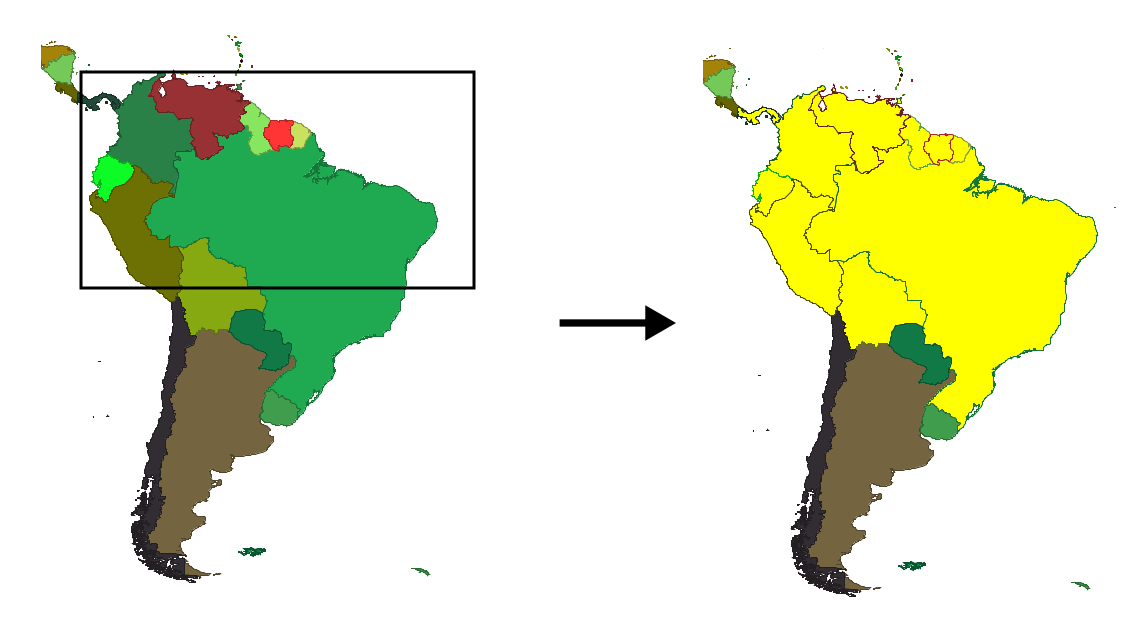
\includegraphics[width=\textwidth]{databases/Selection.png}
\caption{\small Manual selection of features by defining a rectangular region.}
\label{Fig:Selection} 
\end{figure}


A query can also be used to extract certain information from a database according to our needs, and to later create a new layer with it. This operation is very useful when the database contains a large amount of data, but we only need a part of those data. We might create a subset based on spatial criteria (for instance, if the database contains information for the whole world and just want the one corresponding to a given country), a thematic one (the database contains many attributes associated to teach feature, but only a few of them are of interest to us), or a combination of both. To extract that information and create a subset of the original data, we will use a query.

Let's see some more examples of queries. Let's assume that we have a layer with the world countries, and a set of economic and social parameters associated to each of them. For each country, we also have a polygon representing its boundaries.

We can make queries like the following ones:

\begin{itemize}
 \item Which countries have a GDP larger that Spain's one?
\item Which countries have grown economically during the last year?
\item Which countries have a population of more than 200 million people? 
\end{itemize}

In this queries, we are not using the spatial component (we do not need the polygon associated to each country). We could make those queries if we had country data without any spatial component, and using a regular database with no spatial capabilities.

Queries might include several criteria. For instance:

\begin{itemize}
 \item Which countries that have grown economically during the last year have a population of more than 40 million people?
\item In which countries where English is spoken population increased during the last year?
\end{itemize}

To express this queries in a way that can be later adapted to a query language, we need to use \textbf{logical operators}. The above queries would be rewritten as follows.

\begin{itemize}
 \item Which countries have grown economically during the last year \emph{and} have a population of more than 40 million people?
\item In which countries is English spoken \emph{and} the population increased during the last year?
\end{itemize}

Query languages that can be used to communicate with the DMBS support this operators for queries.

If the DBMS is spatial and \emph{understands} that certain columns of a table contain spatial information, it will support queries that use that information, such as the following ones:

\begin{itemize}
\item Which country spans the most degrees of latitude?
\item How many countries are completely contained in the southern hemisphere?
\item Which countries are located at less than 2000 km from Spain?
\end{itemize}

To respond to these queries, we just need to analyze the spatial component, and we do not need the rest of the attributes data. These queries are purely spatial. Although they extend what we had done before, we are not adding here any new way of studying geographical data that was not possible without a GIS. We could respond to those queries using just a classic paper map.

The true power of spatial queries is to allow querying both the thematic and the spatial component. For instance, with queries such as these:

\begin{itemize}
 \item Which countries in the southern hemisphere have a population density higher than the one of Peru?
\item How many countries with a population of more than 10 million people share their borders with Russia?
\end{itemize}

These queries require analyzing the thematic component, and at the same time include criteria that are based on the spatial and topological relations of the associated geometries.

Queries can include \textbf{several layers}. For instance, if along with the countries layer that we have been using, we have a layer with rivers, we could respond to a query such as \emph{Which countries does the Nile river cross?}. This is be a purely spatial query that uses two layers.

Table joins, which were discussed for regular databases with no spatial data, can also be performed with a spatial criteria. These are known as \textbf{spatial joins}.

Here is an example of a spatial join. Suppose that we have a layer with world cities and the layer with countries that we have been using in previous examples. We can define a relation between the two corresponding tables, which will associate to each city all the attributes of the country it belongs to. A field with the country name in both tables is needed for that, to use it as the linking point. 

However, even if we do not have such a field, we can join the tables if we have spatial data for both cities and countries. All cities that belong to a given country must be located within its boundaries. This can be used to define the relation between the tables, and we can know which country it belongs to, just by finding the polygon from the countries list in which the points representing the city is located.


\subsection{Spatial indexes}

If we make a query to a spatial database, responding to it might involve a large number of operation. For instance, if we want to know which countries have a population of more than 10 million people, we need to read the population of every single country in our table and compare it to that value. If the table has a large number or records, the query might take long to be processed. We can clearly see that this is not the optimal way of processing a query.

By using what is known as \textbf{indexes}, we can reach the data that will form the response of our query in a shorter time, without having to pass through all the data contained in the database.

This is easy to understand with an example. Imagine a telephone book. It contains a large number of entries, but you can easily find a name without having to read them all. This is because a) the data is ordered (\textbf{indexed}) in a particular way (alphabetically) and b) you know how to use that indexing (you know the order of letter in the alphabet). With that, you know that it does not make sense to search for Peter Johnson in the pages that correspond to letter A or B, and you can skip them.  

Apart from indexes for numerical or alphanumerical values, which are easy to create, another type of indexes, known as \textbf{spatial indexes} are of great importance in the context of GIS. The concept is similar to non-spatial indexes, and serve the same purpose: to \textbf{optimize searches using a correct data structure}, in this case based on its spatial component.

We will use another example to help understand how an spatial index works. Suppose that we are using our layer with countries and the want to find those that are located at less than 2000 km from of Spain. How would we proceed to response to this query? 

A naive approach would be to measure the distance between Spain and all the remaining countries, then select those at a distance of less than 2000 km. We would get the correct result, but this approach is far from optimal. 

Finding a better approach is easy. For instance, with a little knowledge of world geography, we can immediately exclude all countries in America. We can be sure that they will not be part of the response, since the distance between Spain and America is already larger than 2000 km. We do not know the distance between those countries and Spain, but we are sure that it will be more than 2000 km. Therefore, it makes no sense to measure the distances to all of them.

That knowledge of world geography that allows us to reduce the number of countries to work with is actually like a spatial index. It cannot be used to respond to the query, but it \textbf{provides an approximation that makes it easier to respond to it}. We can discard a large number of countries, and then perform the most costly operations (the measurement) with just a subset.

Thanks to spatial indexes, queries are more efficient and we can work with larger datasets.

Spatial indexes are stored along with the data they refer to, whether in separate files or inside the database itself. Spatial DBMS have \textbf{built-in capabilities to compute spatial indexes} and store them, and once they have been computed, they are used whenever the DBMS has to respond to a spatial query.


\pagestyle{empty}


\chapter{Spatial analysis}



\pagestyle{fancy}

Analysis is one of the key capabilities of GIS. Spatial analysis is the \textbf{quantitative analysis of phenomena, considering the geometric, geographical or topological properties of their elements}. Properties such as position, distance, or area are relevant when performing spatial analysis.

We perform spatial analysis when we use a classic printed map to search for the highest peak in a given map sheet, read the elevation of a given element such as a city, or plan a turistic activity checking the places to visit and how to move between them using the best roads or following the fastest route. Of course, we can also perform this kind of operations within a GIS.

Analysis generates new data, and that data can be in the form of \textbf{new layers, tables, or simple values}.

The result of an analysis might express \textbf{the same variable} as the original data (for instance, computing the average value), or \textbf{a different one} (for instance, if we compute a slope layer from an elevation layer).

Spatial analysis requires spatial data, which can be of a \textbf{single type}, or, instead, of \textbf{multiple types that are combined}. For instance, in the case of finding the highest point in a map, the result is just a coordinate and the only variable used is the elevation. In the case of computing the average elevation of a city, two variables are used: the elevation and the space occupied by the city (defined, for instance, by a polygon with its boundaries). Although all that information is traditionally contained in a single map sheet, in a GIS they will be in separate layers, both if which will be inputs for this particular analysis.

Analysis in a GIS gives us answers to questions that can be:

\begin{itemize}
 \item Related to position or extension.
\item Related to shape or distribution.
\item Related to spatial associations.
\item Related to spatial interactions.
\item Related to spatial variation.
\end{itemize}

\section{Some examples of spatial analysis}

The following sections describe some common types of spatial analysis.

\subsection{Spatial queries}

We already discussed queries in the chapter devoted to databases.

Queries can be combined with other analysis tools, for instance, to \textbf{select} a subset of feature with which we will later perform some other analysis.

\subsection{Topological analysis}

Queries can be refered not just to the position of geographical elements, ut also to their \emph{relation with other elements}. If we have topological information, we can perform analysis that responds to questions such as:

\begin{itemize}
\item How can I reach a give coordinate from my current position using the existing road network? 

\item Which countries share their border with France?
\end{itemize}

\subsection{Measurement} 

Spatial properties can be quantified and measured. Among the most basic ones, we find length, area, perimeter or shape factors. More elaborated ones such as slope or multiple indices derived from basic masurements can also be computed with the help of a GIS.


\subsection{Combination}

One of the most typical procedures within a GIS is the \textbf{combination and overlay} of layers. The separation of geographical data into layers facilitates this kind of operations, and turn GIS into the optimal platform to perform any analysis that requires combining information from different variables.

In the case of vector layers, overlay operations such as \textbf{union, intersection, difference or clipping} are frequently used. Figure \ref{Fig:Intersection} shows an example of an overlay operation between polygon layers.

\begin{figure}[!hbt]   
\centering
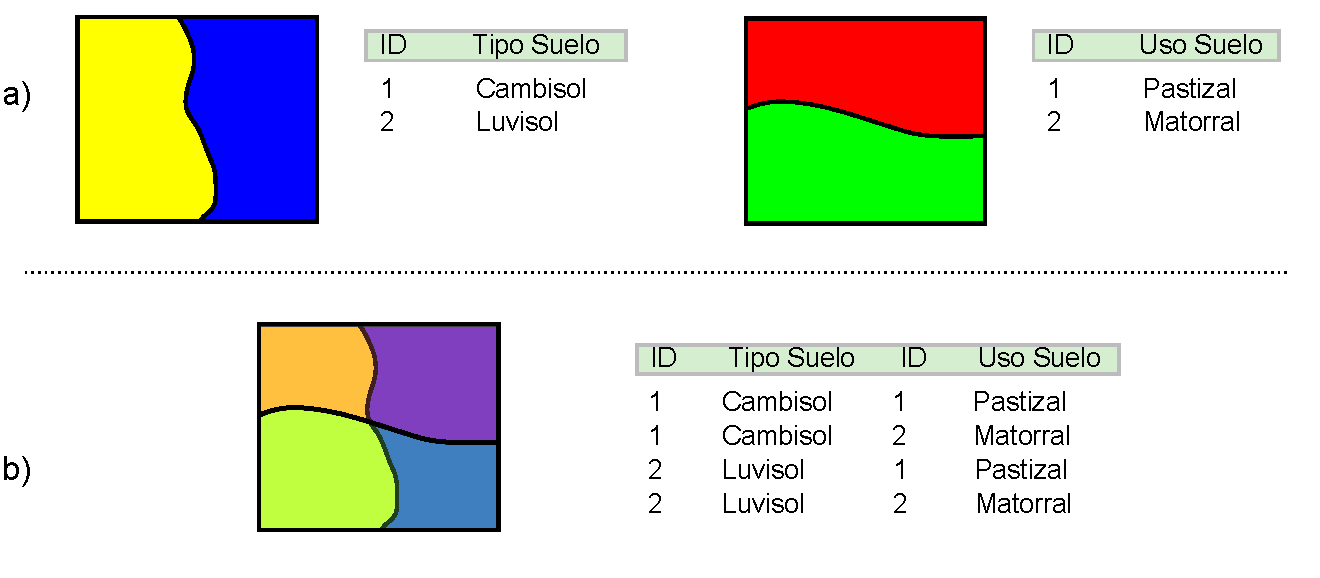
\includegraphics[width= \columnwidth]{Analysis/Intersection.pdf}
\caption{\small Intersection between two polygon layers.}
\label{Fig:Intersection} 
\end{figure}

\subsection{Transformations}

We include in this group a large set of operations that alter the input data in different ways. Among them we find \textbf{coordinate transformations}, \textbf{simplification of geometries} or the \textbf{creation of influence areas (buffers)}. These transformations may affect both the spatial component and the thematic component of the data. 

A particular case, already mentioned in a previous chapter, is the \textbf{conversion between representation models}. Figure \ref{Fig:Conversions} shows an example of this. Starting with a scanned map (a raster layer) with contour lines, these can be traced and a vector layer created based on them. The lines in that vector layer can be later converted into a raster DEM using interpolation techniques. From the raster DEM it is possible to obtain contour lines at an arbitrary contour distance (of course, within the level of detail of the original data).

\begin{figure}[!hbt]   
\centering
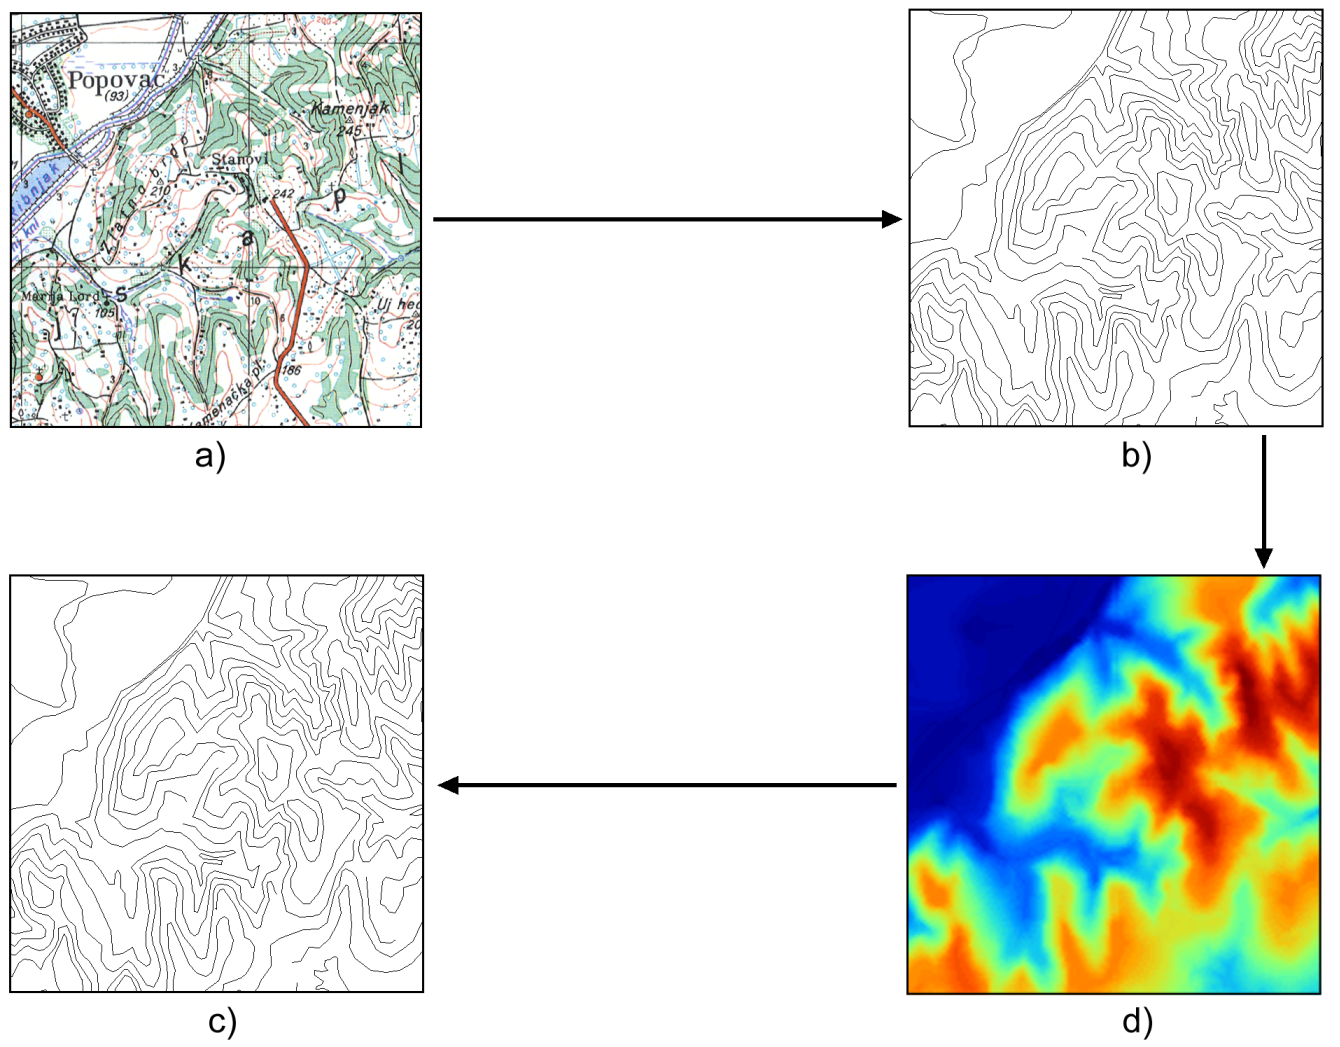
\includegraphics[width= \columnwidth]{Analysis/Conversions.png}
\caption{\small Conversion between representation models for an elevation layer.}
\label{Fig:Conversions} 
\end{figure}

\subsection{Terrain analysis}

Terrain analysis is one of the most powerful capabilities we find in GIS. From basic parameters such as \textbf{slope} or \textbf{aspect}, to highly specific morphometric ones, and passing through a large collection of tools for \textbf{hydrological analysis}, a vast array of analysis capabilities is available in this field.

\subsection{Descriptive statistics}

The common elements of classic statistics have their equivalents when working with geographical data, and they allow us to \textbf{quantitatively describe} the data we work with. Here we include centrality and dispersion measures,  pattern analysis, and many others. These can be themselves used in hypothesis testing, in case there is a spatial component involved.

These statistical values allow us to respond to questions such as:


\begin{itemize}
\item Is average height a constant value across a given country?

\item Is there a predominant movement direction for individuals of a given species, or do they move erraticaly?
\end{itemize}

\subsection{Inference}

Another important statistical analysis in GIS is the one that helps infering the behaviour of variables and their evolution.

\textbf{Change modelling} is one of the many fields that are rapidly evolving thanks to the help of GIS.

\subsection{Optimization and decision-making}

The layered structure of geographical information in a GIS, which, as we have seen was ideal for overlay operations, provides also an optimal framework for estudied the combined effect of multiple platforms. GIS is the perfect framework for \textbf{multiple-criteria analysis}.

Questions such as the following ones can be responded using a GIS:

\begin{itemize}
\item Which one is the best place to build a new power station considering its effect on the environment and the people living close to it?

\item Where should a hospital be located to provide the best possible service to the inhabitants of a given region?
\end{itemize}


\section{Particularities of spatial data for its analysis}

Spatial data has some great potential thanks to its particular properties, but at the same time these properties might \textbf{limit or condition} working with them. In some cases, they might represent problems that have to be considered when analyzing them; in others, they are just something that anyone working with them should know, but that are not problematic \emph{per se}.

\subsection{Scale}

We can study geographical information at \emph{different scales}, and depending one we use, the results we will otain will be different. For this reason, apart from considering scale when rendering and visualizing geographical data, the \textbf{analysis scale} should be considered as well when performing any analysis.

The analysis scale should depend on the \emph{data properties} (accuracy, data type, etc.) and the \textbf{analysis to be performed} with them.

This can be easily understood with the help of \ref{Fig:Scales}. If we want to categorize the form of terrain at a given point, we need to analize the elevation of the point and also the elevation in its surroundings. Depending on the size of that analysys <<window>> around the center point (which is what defines the analysis scale), the results can be very different. In the image, for a small value of the analysis radius, the terrain will be categorized as being a peak. For a larger region, however, it will be considered the bottom of a valley.



\begin{figure}[h]   
\centering
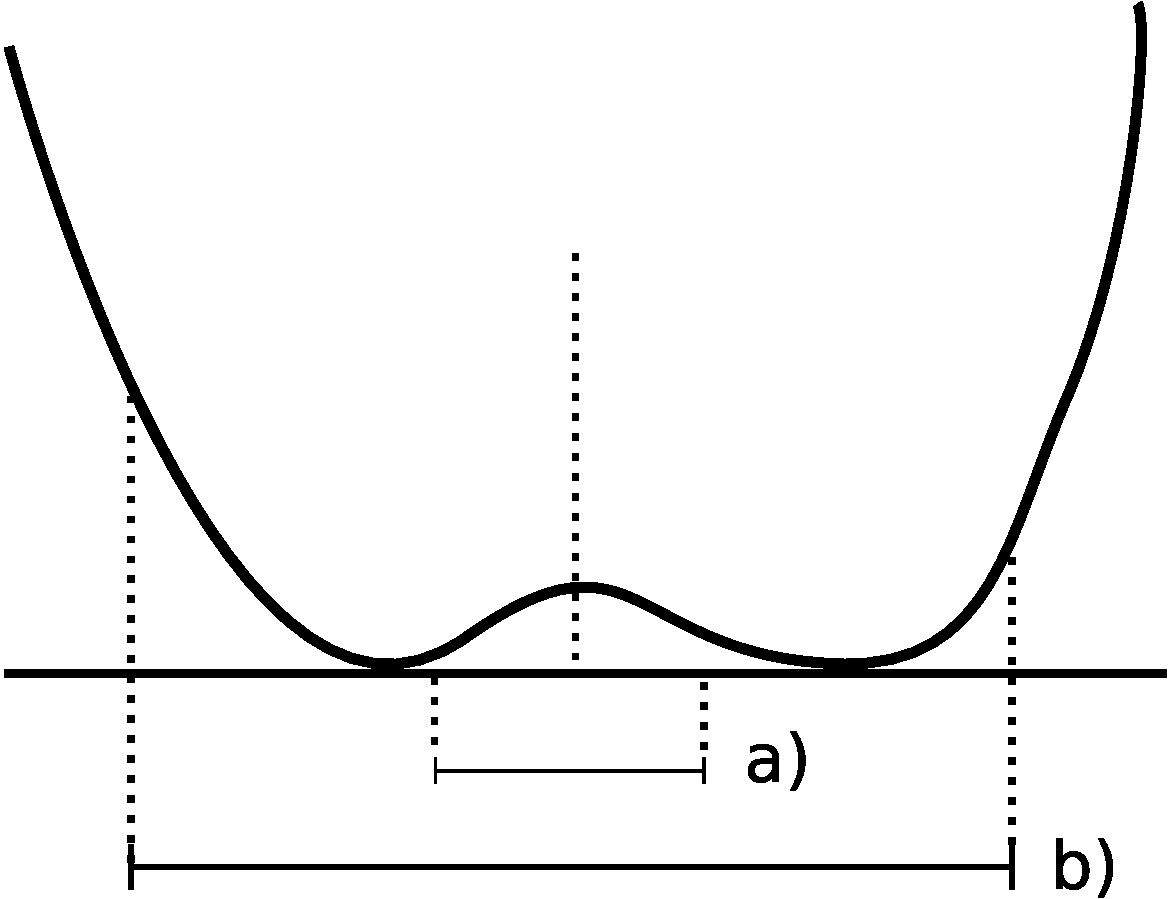
\includegraphics[width= .45\columnwidth]{Analysis/Scales.pdf}
\caption{\small Depending on the analysis scale, the form of the terrain can   be classified as a peak (a) or a valley bottom (b).}
\label{Fig:Scales} 
\end{figure}

Therefore, we must <<look>> at the terrain at the correct distance for which the information that it gives us is the most interesting and correct for the kind of analysis that we are performing. Apart from the fact that there is an optimal analysis scale for each type of analysis, it is also interesting to work at \textbf{multiple scales}, since that will provide us more information than what we can obtain working only at a single scale.

Another example of how the analysis scale affects the analysis result is found in the case of \textbf{taking measurements}. As it can be seen in figure \ref{Fig:Fractal_line}, the measurement unit (which is implicitely defined by the level of detail of the data) that is used causes the results to be different. 

\begin{figure}[h]   
\centering
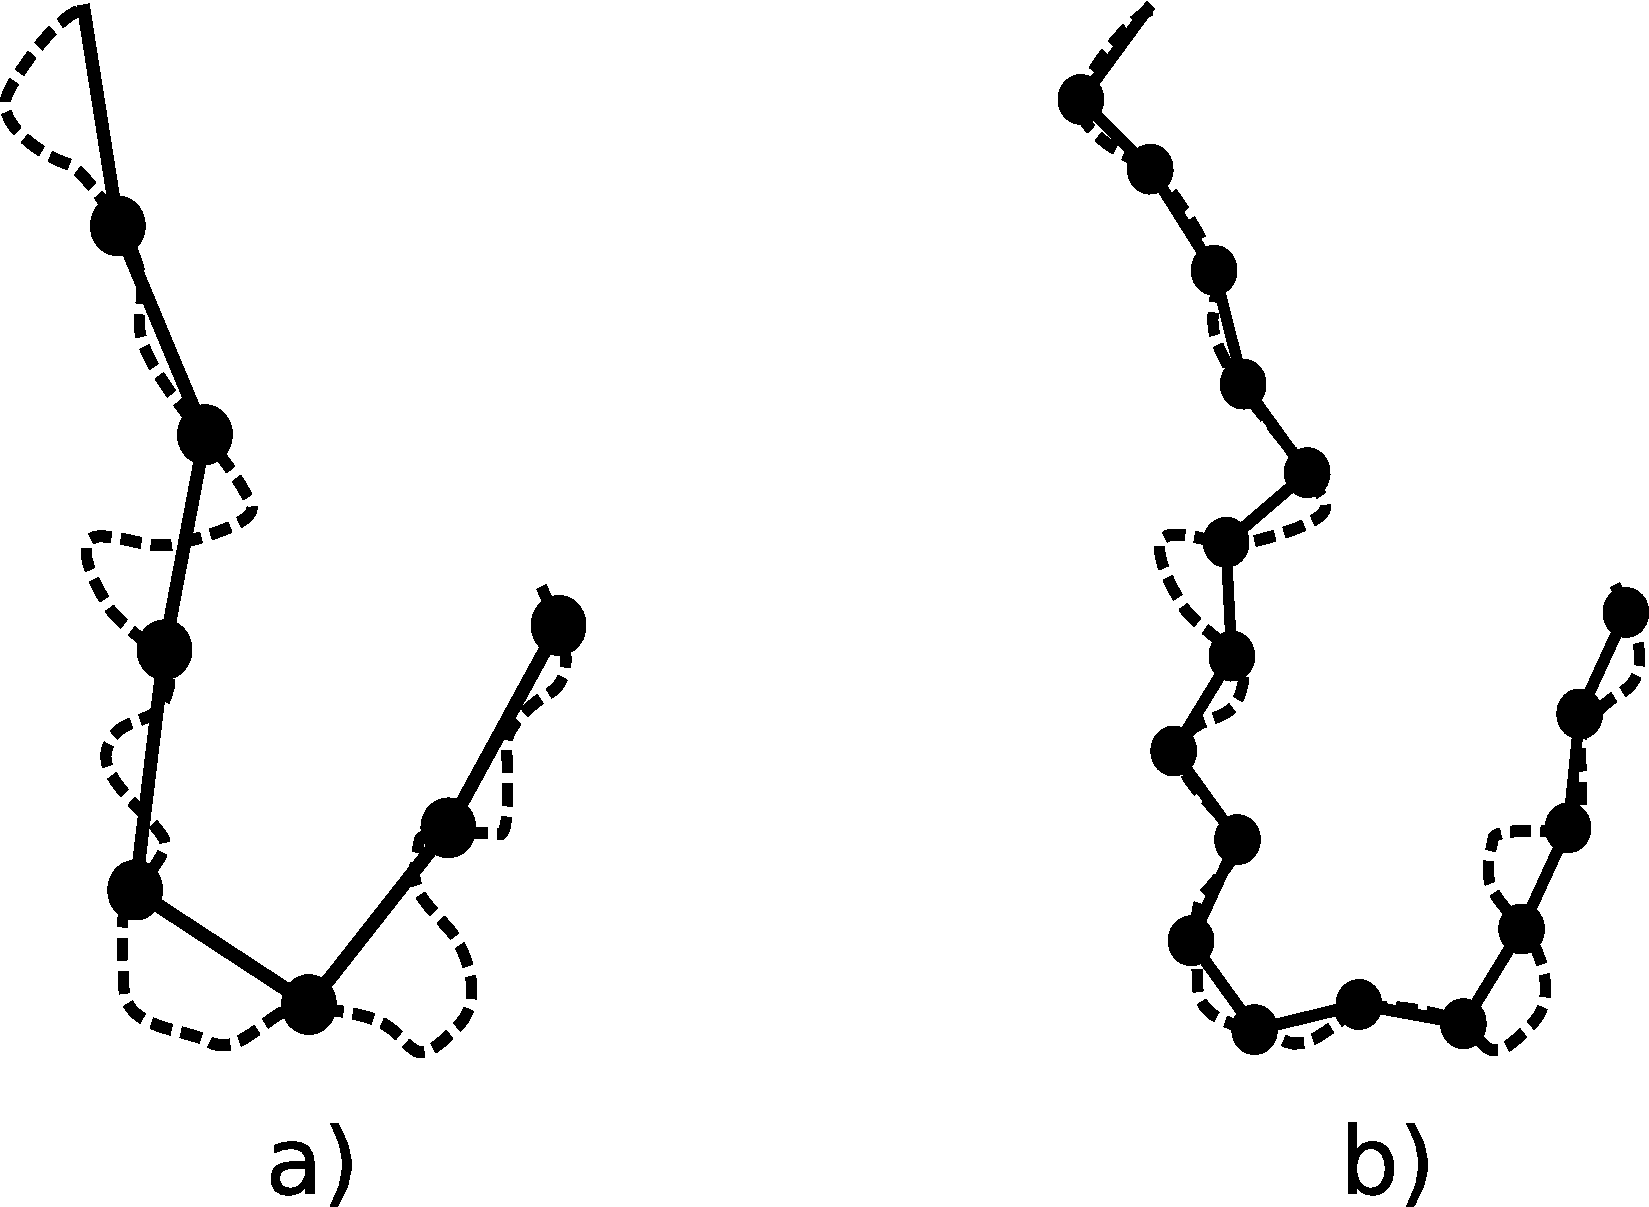
\includegraphics[width= .45\columnwidth]{Analysis/Fractal_line.pdf}
\caption{\small Measurement unit affects the value of the measurement.}
\label{Fig:Fractal_line} 
\end{figure}

A vlue by itself might not have mening if it is not accompanied by the scale that was used to obtain it.

The concept of \textbf{fractal} has a direct link with this.


\subsection{The Modifiable Areal Unit Problem}


Many of the variables that with which we work in a GIS \textbf{cannot be measured at a single point}, and they must be \textbf{aggregated for a given area around that point}. Examples of that are the percentage of the population within a given age range, or the population density. 

Areas defined to work with these variables are \textbf{esentially arbitrary}, such as countries, counties, districts, etc., and they are defined without taking into account any criteria related to spatial anlysis. Using different areas (different units for computing the values of the variable) will yield different results.

This problem is known as the \textbf{Modifiable Areal Unit Problem} (PUAM). Solving or reducing its effect is complex, and no solution exists that can be applied in all cases, but whenever we work with this type of geographical data, it is important to keep in mind that there will be a source of statistical bias that cannot be neglected.

Another problem relateb with the PUAM is the so-called \textbf{ecological fallacy}, which result from (wrongly) assuming that the values computed for a given area can be assigned to the individuals of the population within that area. This would be true only in the case of complete homogeneity.


\subsection{Spatial autocorrelation} 

\textbf{Spatial autocorrelation} is the \textbf{correlation of a variable with itself}, in such a way that values of the variable at any point are correlated with values of that same variable in close-by points. For instance, in the case of temperature, points close to a heat source will have a higher temperature that those far from it or closer to a cold spot. If we study the distribution of an infectious disease, reported cases are likely to appear grouped, and a large number of them normally cause the neary populations to also be largely affected by the disease.

Another way of expressing this is using the well-known \textbf{Tobler's First Law of Geography}, which states that <<everything is related to everything else, but near things are more related than distant things>>.

In the above cases, sppatial autocorrelation is said to be \textbf{positive}. However, it can be also \textbf{negative}, if higher values are surrounded by lower ones, or there can be no correlation at all, when values in separate points are \textbf{independent} and do not affect each other regardless of distance.

Figure \ref{Fig:Autocorrelation} shows three raster layers which demonstrate the above types of spatial autocorrelation.

\begin{figure}[!hbt]   
\centering
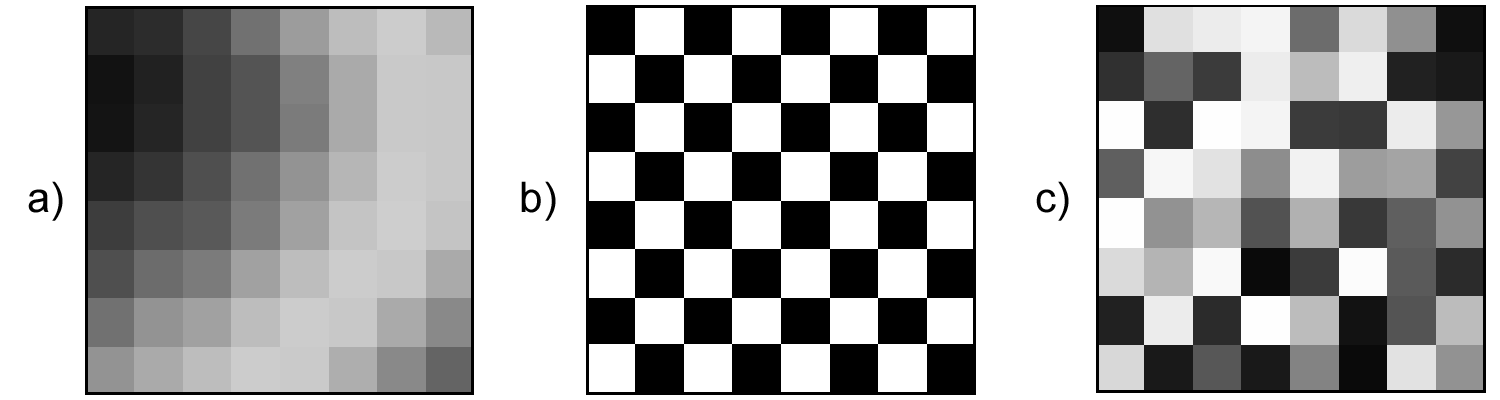
\includegraphics[width=\textwidth]{Analysis/Autocorrelation.png}
\caption{\small a) Positive spatial autocorrelation. b) Negative spatial autocorrelation. c) No spatial autocorrelation (independency).}
\label{Fig:Autocorrelation} 
\end{figure}

The existence of spatial autocorrelation has many important consequences.

First, many of the most commmon statistical analyses assume depency of the variable that is being studied. Since there is a dependency on the spatial component, this component has to be introduced as another variable to consider, in order to ensure that results are sound.


Something similar happens when data have a \textbf{spatial trend}(values of a variable depend on the position, like, for instance, temperature values, which show a clear trend as latitude changes), since that also invalidates the assumption that data are independent.

If positive correlation exists, \textbf{statistical inference is less effective}. The same number of observations contain less information about the phenomena represented by the variable.

The consequences of spatial autocorrelation, however, are not only negativa. If points located in the vicinity of a given one are related to it, and the value of a variable are affected by that proximity, that can be used to \textbf{estimate values} at any point, knowing the values in a set of naerby points. That is the fundamental idea behind \textbf{interpolation methods}.


\subsection{Structure}

Both the data itself and the properties of the phenomeon they represent (such as the aforementioned spatial correlation) have some sort of structure. This structure can have a relevant effect on the analysis results, and should be taken into account.

The two basic statistical concepts related to the spatial structure of a process are \textbf{stationarity} and \textbf{isotropy}. Stationarity indicates that the process is \textbf{translation-invariant}. That is, its properties are constant across the whole space and there is no spatial trend. Isotropy means that the process is \textbf{rotation-invariant}, and happens in the same way in all directions.

\subsection{Border effects}

The areas in which we perform spatial analysis \textbf{have boundaries}. These might be artificial ---for instance, the limit of the aerial photograph we are working with---, or natural ---if we study a forest that is close to a lake, the shore will be limit of the forest. Boundaries \textbf{distort the result of analysis}, specially for those variables that have to be aggregated (density, etc., as we saw for the case of PUAM)

In some cases, the border effect might manifest itself only for those point close to the border. In others, however, \textbf{all the points related or somehow connected to the border} might be affected, regardless of the distance to it.

\pagestyle{empty}
\chapter{Visualizaci�n y representaci�n de datos espaciales. }


\pagestyle{fancy}

When working with a GIS, most of the time we will visualize the data we work with. Although certain data, such as satellite images or maps from a map server, include their own rendering and can be visualized \emph{as they are}, in most cases us the user of a GIS who defines the way geographical data is rendered. In other words, the GIS user \textbf{takes the role of the cartographer}, and for this reason must be familiar with the ideas and techniques used by cartographers.

Along with the concepts and tools from classic cartography, GIS include elements from what is known as \tetbf{scientific visualization}, such as \textbf{interactivity} or \textbf{multidimensional data rendering}. This approach, richer the classic one from cartography, is known as \textbf{geovisualization}.

In this chapter, we will see some fundamental ideas about data visualization, and how they are applied to both the traditional field of cartography and the GIS and geovisualization context.

\section{Basic ideas about data visualization}

When we visualize any kind if geographical information, whether on a computer screen or on a printed map, we are using a \textbf{visual language} to convey that information. 

The study of signs of a language is called \textbf{semiology}. In the case of a visual language, we have a \textbf{graphic semiology}. This semiology works with the signs of the language that we use to visualize geographical data, and helps us understand why and how visual elements serve their purpose of correctly conveying the information from which they are created.

\subsection{Visual variables}

Visual elements have several properties that can be used to transmit information. Depending on the case, some of them might more suitable than others.


\begin{figure}[!hbt]
\centering

\includegraphics[width=\columnwidth]{Visualization/VisualVariables.pdf}
\caption{\small Usage of visual variables. From left to right: position, shape, size, hue, value, texture and orientation.}
\label{Fig:VisualVariables} 
\end{figure}

These properties are known as \textbf{visual variables}, and are applied to the geometric elements used to visualize geographical information. Those elements can be differentiated using the following visual variables, which are shown in figure \ref{Fig:VisualVariables}: position, shape, size, hue, value, texture and orientation.

Usage of \textbf{Position} is rather restricted in the case of a map, since the real position of the element to be rendered should be respected. It is seldom used. 

The \textbf{shape} is defined by the perimeter of the object. This variable is mostly used in the case of point data, using a symbol of a given shape located at the exact coordinates of the point to be rendered. It is difficult to apply to linear symbols, and in the case of areal symbols it requires altering the shape of the symbol itself.

\textbf{Size} indicates the dimensions of the symbol. In the case of points, it can be applied by changing the size of the symbol itself. In the case of lines, changing their thickness is the most usual way of using this visual variable on them. It is not used in areal symbols, except for the case of using a texture fill, in which the size variable is applied to the texture and not to the symbol itself.

Size \textbf{alters how other visual variables are perceived}, specially in the case of small sizes.

\textbf{Texture} refers to pattern used to fill the body of the symbol. It can be applied to lines, using dash paterns, but it is mostly applied to areal symbols.

Color is the most important of all visual variables. Two of its components can be used as individual visual variables themselves: hue and value.

\textbf{Hue} is what we usually call color. That is, the name of the color (blue, red, green, etc.)

Hue can be \tetbf{can be altered by the hue of surrounding elements}, specially in small symbols. Although human perception has a great sensitivity to it, it might be difficult to identify in small symbols, and it can be wrongly identified if the symbol has other larger ones with different hues in its surroundings.

\textbf{Value} defines the darkness of the color. For instance, light blue and dark blue have the same hue, but they have different value.

Differentiating between two symbols can be more difficult depending on the type of symbol. It is easier to in the case of areal symbols, while in the case of linear and point symbols it depends on their size. Smaller sizes make it more difficult to compare values and to extract the information that the visual variable is trying to convey.

\textbf{Orientation} is applied to point symbols, unless they have some sort of symetry that makes it difficult to identify the orientation of the symbol. For areal symbols, it is applied to their texture. It's not applied in the case of linear symbols.

\subsection{Properties of visual variables}

Visual variables can have four basic properties.

\begin{itemize}
	\item \textbf{Associative}. A visual variable is said to be associative if, when applied, doesnt change the visibility of an element. That is, it's not possible to give more important to an element using that visual variable. 
	\item \textbf{Selective}. A visual variable is said to be selective if, when applied, generates different categories of symbols.
	\item \textbf{Ordered}. A visual variable is said to be selective if it can be used to represent a given ordering,
	\item \textbf{quantitative}. When, apart from being ordered, it can be used to express ratios.
\end{itemize}

In the above list, variables are ordered according to the so-called \textbf{levels of organization}. The associative property is at the lower level, while the quantitative one is at the highest. The level of organization of visual variables is relevant when combining them, as we will see later. Also, the level of organization of a variable defines the type of information that the variable can transmit.

Figure \ref{Fig:PropertiesVisualVariables} shows different renderings of a set of point symbols, explaining in each case one single visual variable.

\begin{figure}[!hbt]
\centering
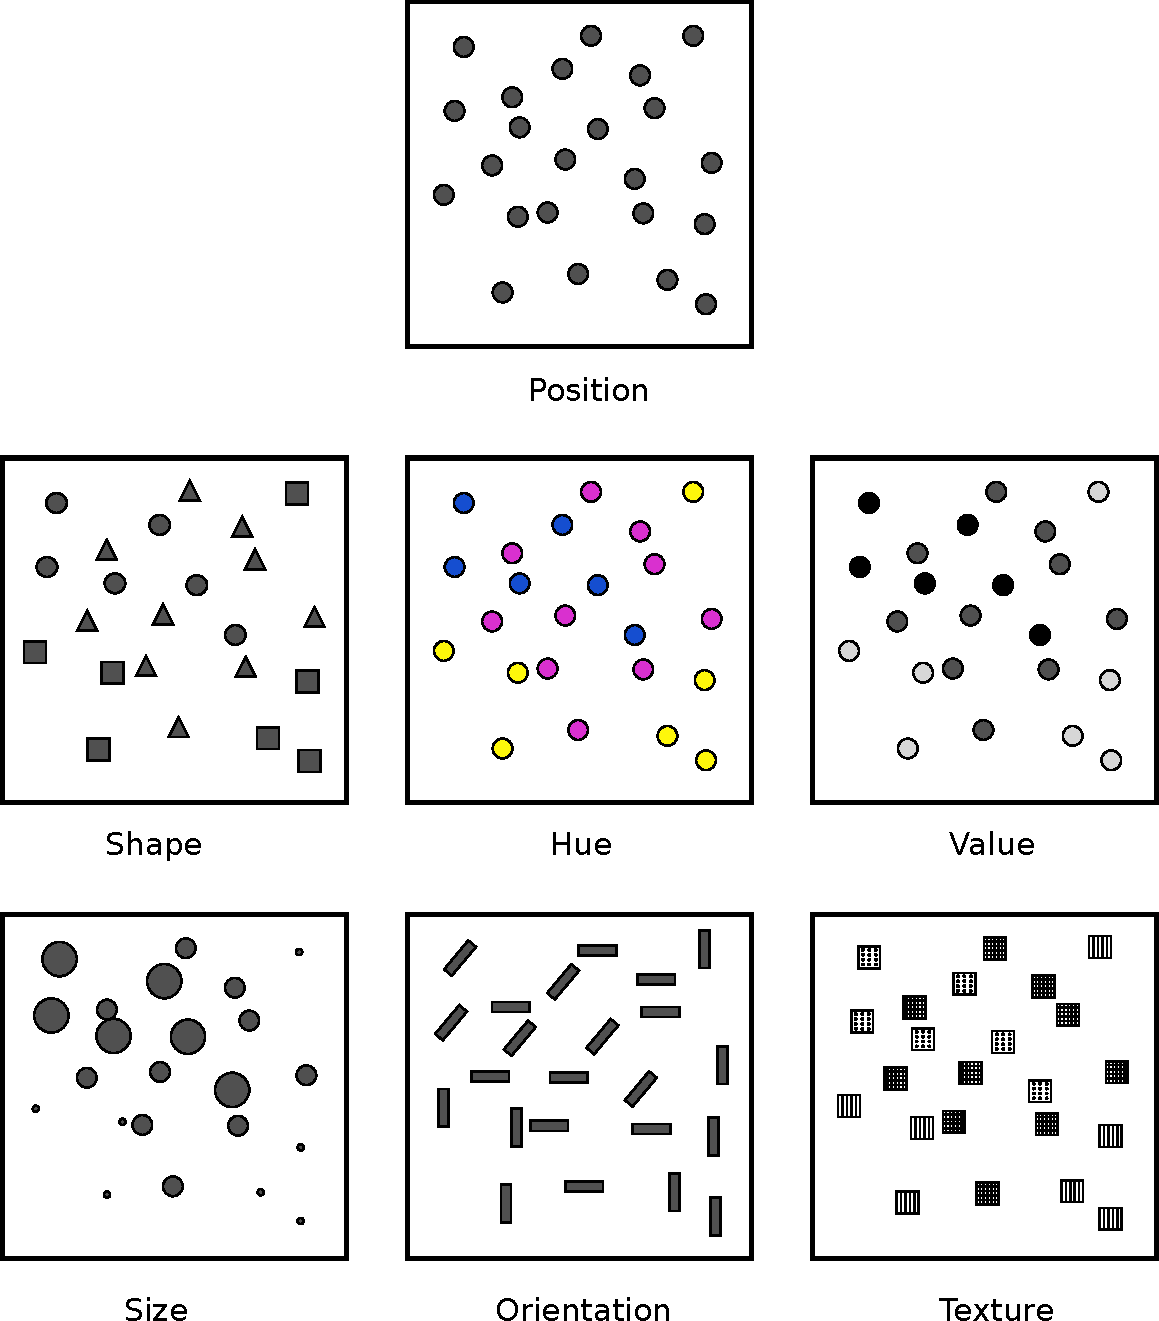
\includegraphics[width=\columnwidth]{Visualization/PropertiesVisualVariables.pdf}
\caption{\small Visualization of a set of point symbols using a single visual variable in each case.}
\label{Fig:PropertiesVisualVariables} 
\end{figure}

Starting with the associative property, we see that, except for size and value, all other visual variables do not make elements to be preponderant in the image. There is not an orientation than can be called more important that the rest of them. The same happens with texture, color, shape or position.

With size, however, it is clear that a larger one gives symbols a more prominent role. In the same way, a larger value (darker color) attracts the attention of the observer much more than a color with a lighter value.

Regarding the selective property, we can say that a variable has if, with a quick look, we can easily identify the elements that belong to a given group, that group being defined by that visual variables. The most clear example of this hue. We can quickly separate from a set of symbols those that are red or yellow. All visual variables, excepting shape, have this property, although it might not be so inmediate to notice that as in the case of hue  have this property. Shape does not make elements form groups spontaneously.


The ordered property is found in those visual variables that we can use to define an ordering. Ony position, texture, size and value have it. For instance, in the image corresponding to the the visual variable hue, we cannot say which element we would place at the beginning  or end of a scale defined by hue itself. With value, however, we can, since that scale would range between the lighter tones to the darker ones, and we can visually differentiate them and sort them.

Finally, the quantitative propery is found in those visual variables that can be used to visually estimate quantities and ratios. Only position and size have it. For instance, we can see that the big circles in the image corresponding to the size visual variables are more or less twice the size of the smaller ones.

Table \ref{Tabla:PropertiesVisualVariables} contains a summary of all this.

\begin{table}[!hbt]
\small
\centering  \label{Tabla:PropertiesVisualVariables}
\begin{tabular}{p{3.6cm}ccccccc}  
 & \rotatebox{90}{\textbf{Position}} & \rotatebox{90}{\textbf{Size}} & \rotatebox{90}{\textbf{Shape}} & \rotatebox{90}{\textbf{Value}} & \rotatebox{90}{\textbf{Hue}} & \rotatebox{90}{\textbf{Texture}} & \rotatebox{90}{\textbf{Orientation}} \\ \midrule   
\textbf{Associative}& $\diamondsuit$ & - & $\diamondsuit$ & - & $\diamondsuit$ & $\diamondsuit$ & $\diamondsuit$ \\
\textbf{Selective}& $\diamondsuit$ & $\diamondsuit$ & - & $\diamondsuit$ & $\diamondsuit$ & $\diamondsuit$ & $\diamondsuit$ \\
\textbf{Ordered}&$\diamondsuit$ & $\diamondsuit$ & - & $\diamondsuit$ & - & - & - \\
\textbf{Quantitative}& $\diamondsuit$ & $\diamondsuit$ & - & - & - & - & -  \\
\bottomrule \end{tabular}
\caption{\small Properties of visual variables.}
\end{table}

Las variables visuales pueden combinarse (por ejemplo representando elementos con puntos de distinto tama�o y tono). Al hacerlo, deben tenerse en cuenta las propiedades de estas del mismo modo que cuando se emplean de forma individual. Las propiedades a reforzar ser�n aquellas que convengan m�s al tipo de informaci�n representado, y deben presentarlas todas las variables a combinar para que el efecto conjunto sea m�s acusado.


\subsection{The perception of visual variables}

The perception of visual variables \textbf{might be altered by the environment}. It is important to study this from two points of view: \textbf{perceptual constancy} (how much we can modify visual elements and their surroundings before they fail to to convey the same information and can be misidentified) and \textbf{perceptive aids} (how we can help visual element to be perceived exactly in the way that we want to)

Perceptual constancy defines how objects are \textbf{perceived in the same way regardless of the changes in the environment}. For instance, if an object is round, such as a wheel, it will have a round shape when we look at it from a perpendicular direction. If we now look at it from a different angle, we will see an ellipse instead of a circle. However, we will not think it is not round, and we will still identify its shape correctly. That is an example of the perceptual constancy of the shape.

Not all visual variables have such a perceptual constancy. When the perception of an element changes even if the object itself does not, a \textbf{perceptual contrast} is said to exist. Perceptual contrast might cause a visual element to be wrongly perceived, and the information that it transmits to be misinterpreted.

The following ones are some of the main ideas about perceptual contrasts to take into account when creating a map:

\begin{itemize}
	\item Size is the visual variable that is more affected by perceptual contrasts. The apparent size of an object might change if it is surrounded by other elements of a different size. This is particularly relevant when using point symbols in a map.	
	\item Values is also altered when other elements with a differnet valu appear nearby, specially if there is a large numebr of them.
	\item Hue is altered by the presence of other hues. In a map, we should consider how the background color might affect the one of foreground symbols. 
	\item Complementary hues, when put together, might cause a <<vibration>>sensation in the border between them.
\end{itemize}

Regarding perception aid, the mosst important factor when creating a map is the \textbf{correct separation between the figure (the foreground objects) and the background}. The properties of the visual variables must to be used to create different levels in the visualization, assigning more relevance to some element in order to focus the attention on the information that they transmit.

To make certain layers (the most relevant ones for the purpose of the map) more visible, a \textbf{correct hierarchy} must be establish with the help of visual variables. This hierarchy will add <<depth>> to the information displayed in the map, and some elements will be perceived as being more important than ohers. Layer ordering already defines a structure and a hierarchy, but that is not enough in most cases, and visual variables should be used to reinforce it.

Figure \ref{Fig:HierarchyMap} shows why a correct hierarchy is needed to create a good map.

\begin{figure}[!hbt]
\centering
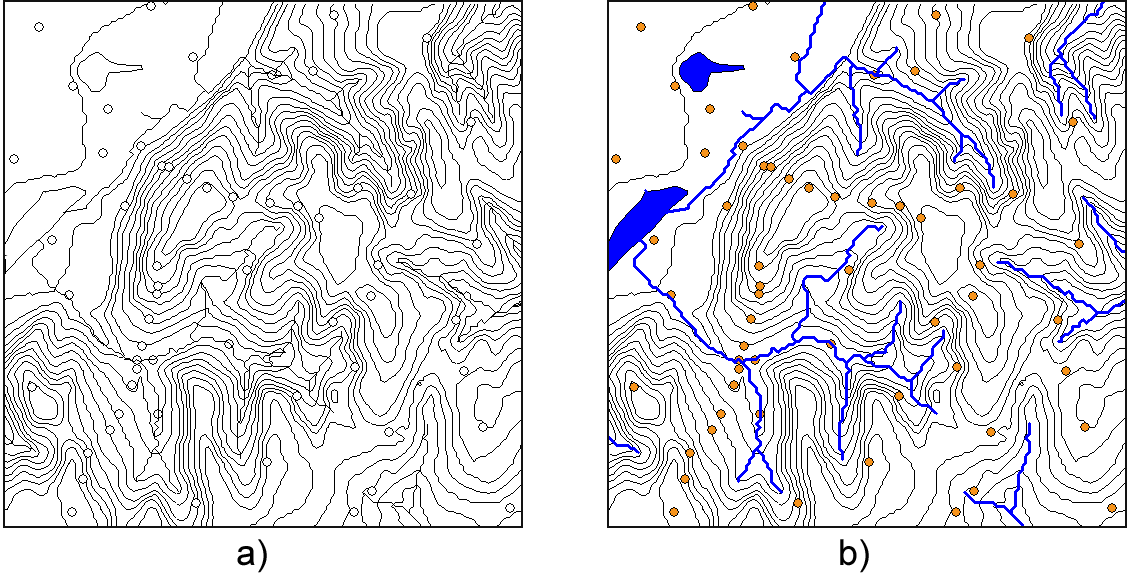
\includegraphics[width=\columnwidth]{Visualization/HierarchyMap.png}
\caption{\small Comparison between a map without hierarchy (a) and a map with a correct hierarchy (b).}
\label{Fig:HierarchyMap} 
\end{figure}


\section{Maps and cartographic communication}

Maps are a method of communication that uses a language with a particular purpose: \textbf{describing spatial relations}. A map is, therefore, a symbolic abstraction of a real-word phenomenom, which implies that it has some degree of simplification and generalization.

The visual language that we have just seen becomes now a cartographic language when it is adapted to the particular case of creating maps, and knowing its rules is needed to create cartography that is later useful for the map user. All these ideas related to map production form what is known as \textbf{cartographic design}.

Cartographic design involves taking decisions (in this case, by the GIS user who takes the role of the cartographer). This decision must be guided by the \textbf{purpose of the map} and the \textbf{public it is target at}, and depending on these factors the cartographer must decide \textbf{the projection} (which not always has to be the original one of the data) 
, the \textbf{scale} (depending on the level of detail and taking into account the limitations of the data), the \textbf{type of map} (we will see more about this later in this chapter), or the \textbf{symbols} to use.

There are two main types of cartography: \textbf{base cartography} (also called \textbf{fundamental} or \textbf{topographic}) and \textbf{thematic cartography}.

Base cartography represents the classic maps that have been created by cartographers during most part of the history of cartography. This type of map serves the purpose of precisely describing \emph{what} is on the surface of the Earth.

Thematic cartography focuses on \textbf{displaying information about a given phenomenon} (a given geographical variable), which can be of any type: physical, social, political, cultural, etc. We exclude from this list those phenomena that are purely topographic, which are the subject matter of base cartography.

We can also say that base cartography represents \textbf{physical elements} (a stream, a coast line, a road, a valley, etc.), while thematic cartography focuses on \textbf{representing values and attributes}.

Thematic cartography uses base cartography (usually included in thematic maps) to help the map user to understand the spatial behavior of the variable being represented, and also to provide a geogrpahical context for it.


\subsection{Types of information and their visualization}

We already know that the thematic component of geographical information can be numeric or alphanumeric, and that numeric variables can be nominal, ordinal, intervals, or ratios. Selecting a correct symbology according to the type of information that we are working with is key to produce an effective map. In particular, we must use a visual variable that has the correct properties (levels of organization) for the variable that we want to visualize.

For instance, the associative property and the the selective property are of interest just for qualitative information, while size is the only visual variable that we can use that has the quantitative property, and, therefore, the only one that should be used to represent ratios.

The following are some of the most important ideas about this, refered to the aforementioned types of information.


\begin{itemize}
	
	\item \textbf{Nominal}. Nominal information is correctly represented using the visual variable shape. This information shows \emph{what} is found in the differnt locations of a map, and not \emph{how much} is found, and it more related to base cartography than to thematic cartography. Using different symbols for point elements and line elements is a common and very effective solution. For the case of areal symbols, hue and texture are the most common solution.

	Alphanumeric information is has similar properties, and the same ideas apply to it as well.
	

	\item \textbf{Ordinal}. Since values of the variable define an order, a visual variable wiwth the ordered property is needed to correctly visualize this type of information
	
	\item \textbf{Interval and ratio}. Visual variables with the ordered property can be used in this case. However, size is a better choice in this case, since it is the only one that has the quiantitative property.

	Values are normally grouped in classes, so the same value of the visual variable (same size of the symbols or same coloro value, for instance) is used for different values of the variable that we are visualizing. There are different strategies for this, which try to maximize the information that the map transmits. The most commons ones are \textbf{equal interval, intervals using percentiles} or \textbf{natural intervals}, which try to minimize the variance within each class.

	Using one or another of these methods can have a noticeable effect in the visualization, as it is shown in figure  \ref{Fig:IntervalClasses}.

	\begin{figure}[!hbt]
	\centering
	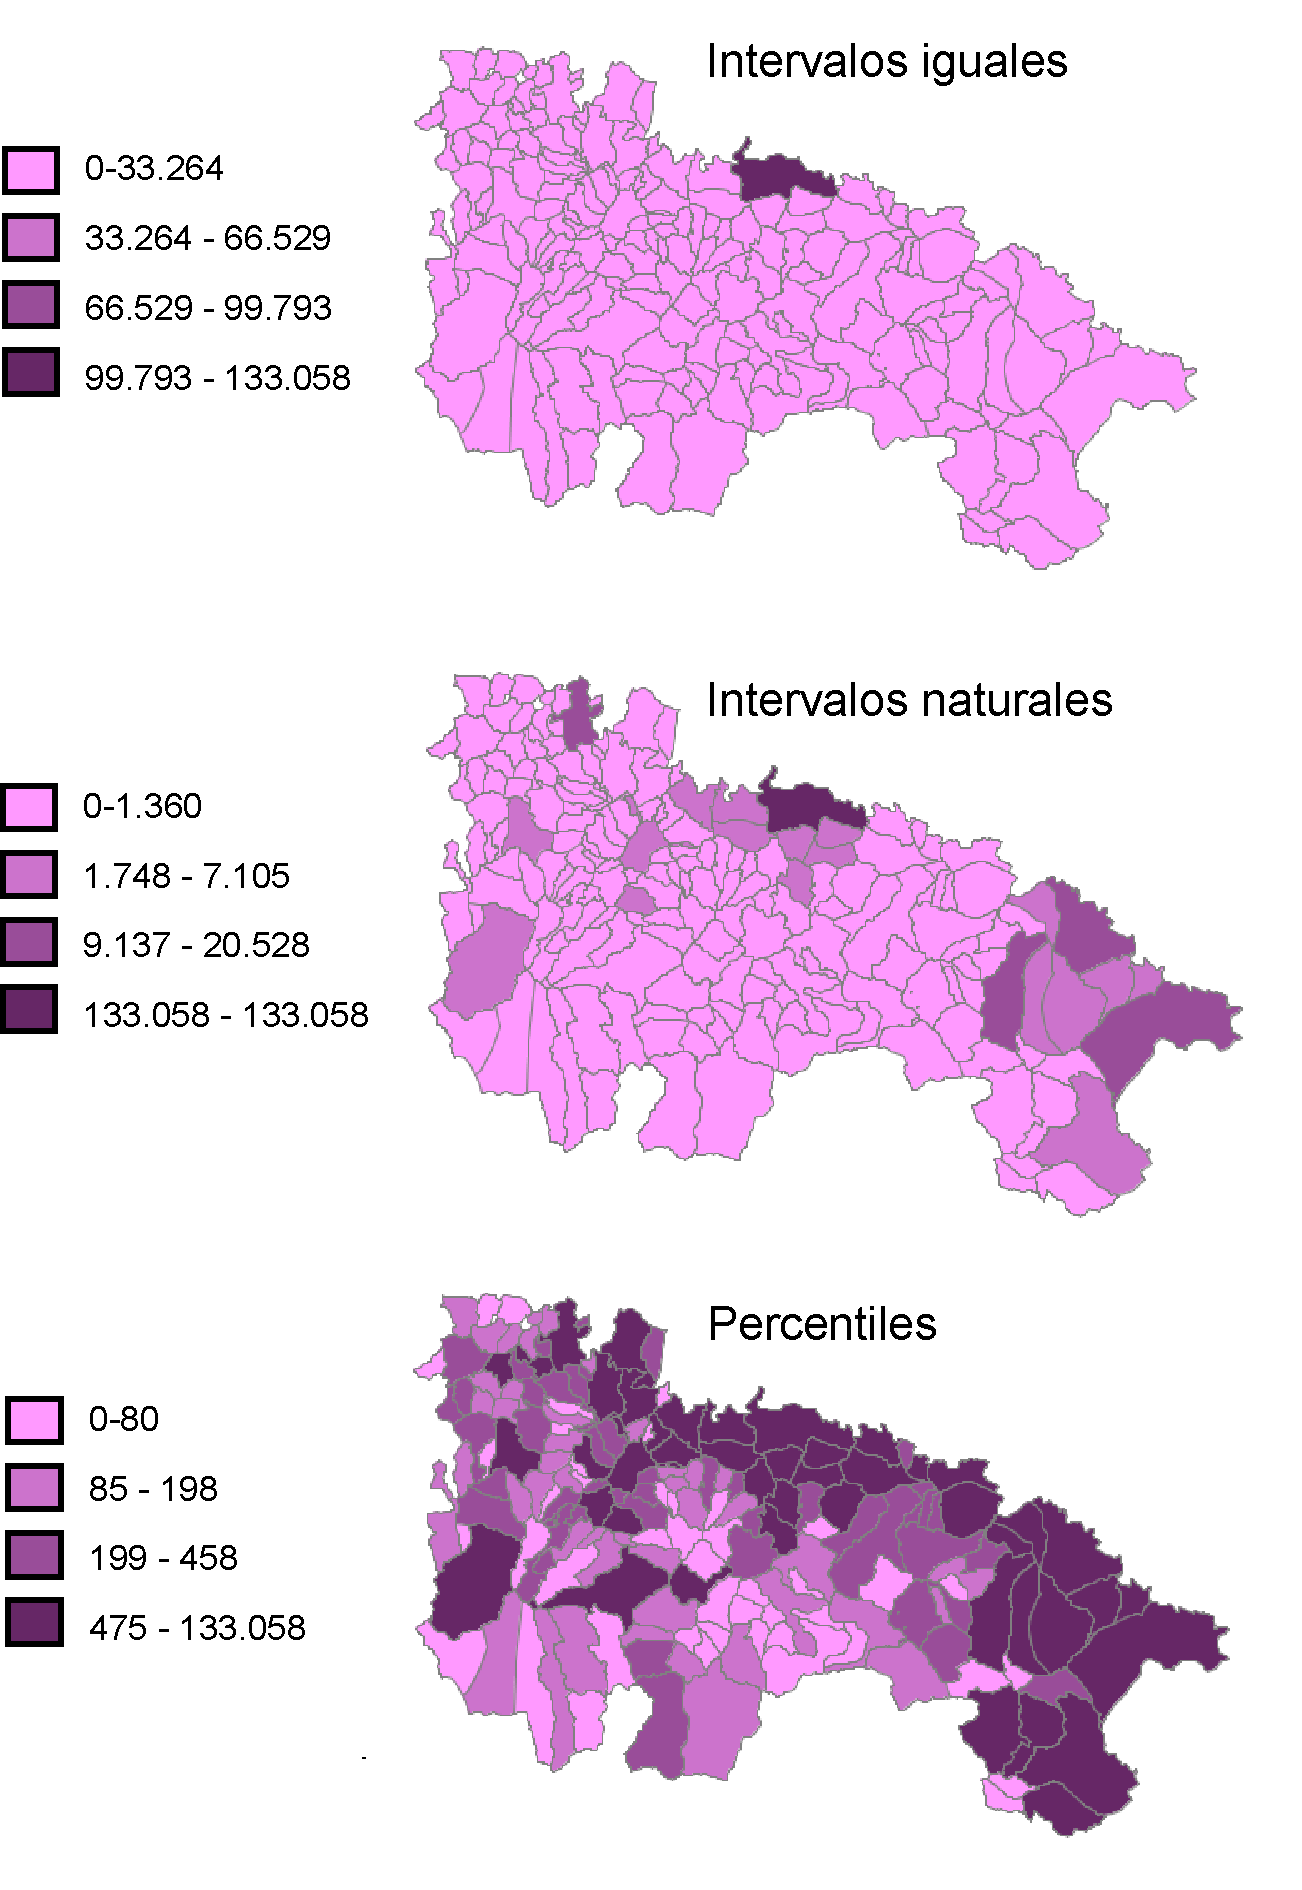
\includegraphics[width=.7\columnwidth]{Visualization/IntervalClasses.pdf}
	\caption{\small Comparison between different methods of defining intervals.}
	\label{Fig:IntervalClasses} 
	\end{figure}


\end{itemize}


It is important to remark that, although levels of organization indicate increasing potential (that is, with a variable such as size or value we can convey all the information that can be conveyed with hue, since they have properties with a higher level), \textbf{it is not always a better idea to use variables with higher level of organization}, and it is not true that they will always be better than those with a lower one. For instance, using the visual variable value for a map with qualitative information (like using a ramp of different tones of blue for a map with soil type information) might not be a good idea, because it has the ordered property, and that might cause the map user to think that there is some hierarchy (that some soil types are <better>> than others), which is false.


\subsection{Map elements. Map composition}

A map is not just the part of it that represents the geographical information, but a set of multiple elements, one of them being the one that contains the geographical information itself.

A \textbf{correct layout of the map elements} is as important as a correct symbology, since these, like symbology itself, are designed to help the map user to better interpret the information that it contains.

The following are the main elements that can be used to compose a map (Figure \ref{Fig:MapElements}):

\begin{figure}[!hbt]
\centering
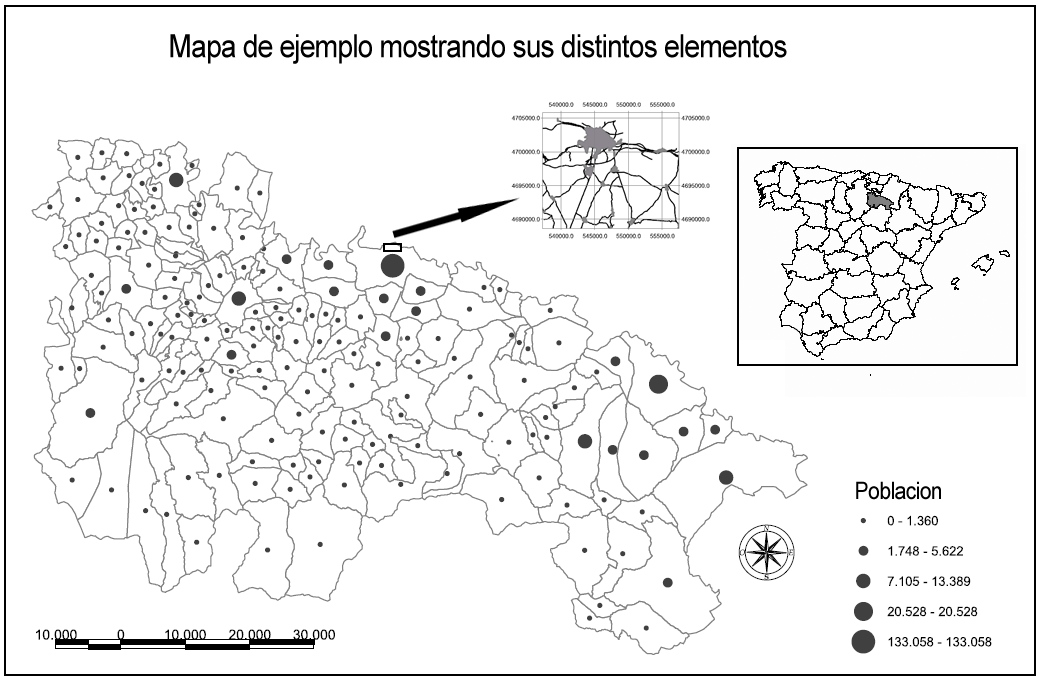
\includegraphics[width=\columnwidth]{Visualization/MapElements.png}
\caption{\small Map with its most common elements.}
\label{Fig:MapElements} 
\end{figure}

\begin{itemize}
\item \textbf{Name or title}. Needed to know the information that is contained in the map.
	\item \textbf{Author}. Individual or organization that created the map.
	\item \textbf{Additional information about the map}. For instance, the coordinate reference system used or its creation data, among others.
	\item \textbf{Data frame}. The frame which contains the rendered geographical information. It is the central element and will use most of the space of the map. 
	\item \textbf{Graticule}. On top of the data frame, it locates the content of our map in the Earth's surface and provides a geographical reference. It also serves the same purpose as the scale, helping to estimate distances. It is usually added at all scales, but it is more relevant in the case of small scales.
	\item \textbf{Legend}. When designing a map, we should try to use a symbology that is as expressive as possible. However, sometimes it is not possible to include all the information with just the symbology itself, and a legend is requried. The legend has to be clear and easy to interpret as well. A legedn that is too large or difficutl to understand is probably telling us that the symbology that we have selected can be improved.
	
	The legend and the data frame form a single unit, and should be together (legend inside the data frame), not separated in different frames or with boundaries between them, unless the data frame uses all the space of the map and it is not possible to visually separate both elements clearly.
	

	\item \textbf{North arrow}. Although by convention have a south-north orientation (north is at the top of the map), it does not always have to be like that. An arrow pointing north or a compass rose help clarifying the map orientation.

	\item \textbf{Scale}. Map scale should be displayed both numerically and graphically (scale bar).
	\item \textbf{Locator map}. It allows to locate the map in a larger geographical context. IT is specially relevant in the case of map series, to show the relation between the current map and the rest of them, acting as an index map.
	\item \textbf{Detail maps}. Used when there is an area that we can show with a greater level of detail. The area that it corresponds to should be indicated as well in the main map. 
\end{itemize}

It is also important that the map \textbf{emphasizes its purpose}, giving more importance to those element that serve it better.

\section{Types of thematic maps}

There are many different ways of visualizing a given variable in a map. Several of them can be combined in a single map, specially if it includes more than one variable. In this case, the combination should strive to obtain the maximum possible clarity for all of them, so the rendering of a variable does not shadow the remaining ones.

In this section, we will describe the following types of thematic maps: proportional symbol maps, point density maps, isoline maps and choropleth maps.


\subsection{Proportional symbol maps}

A propotional symbol map represents \textbf{quantitative variables} using symbols whose size \textbf{is proportional to the value} of the variable. That is, it uses the visual variable size (the only one with the quantitative property), to transmit the value of the variable being represented. If the symbol used is linear (such as a bar), its length is used to scale the values to render. If it is areal, are a is used. That means that, in case of using circles, a value theee times larger than a reference one, will not be rendered with a circle with a radius three times longer, but with a circle with an area three times the area of the reference circle.

Symbol scaling can be done in a continuous way, but it is usually more convenient to use a discrete approach, grouping values in classes and assigning a single size for all values in each class, usually the size that corresponds to the center value of the class. 

To avoid problem when perceiving the size of each symbol, it is important to show in the legend the relation between the different sizes and their corresponing value, as can be seen in figure \ref{Fig:LegendProportionalSymbols}

\begin{figure}[!hbt]
\centering
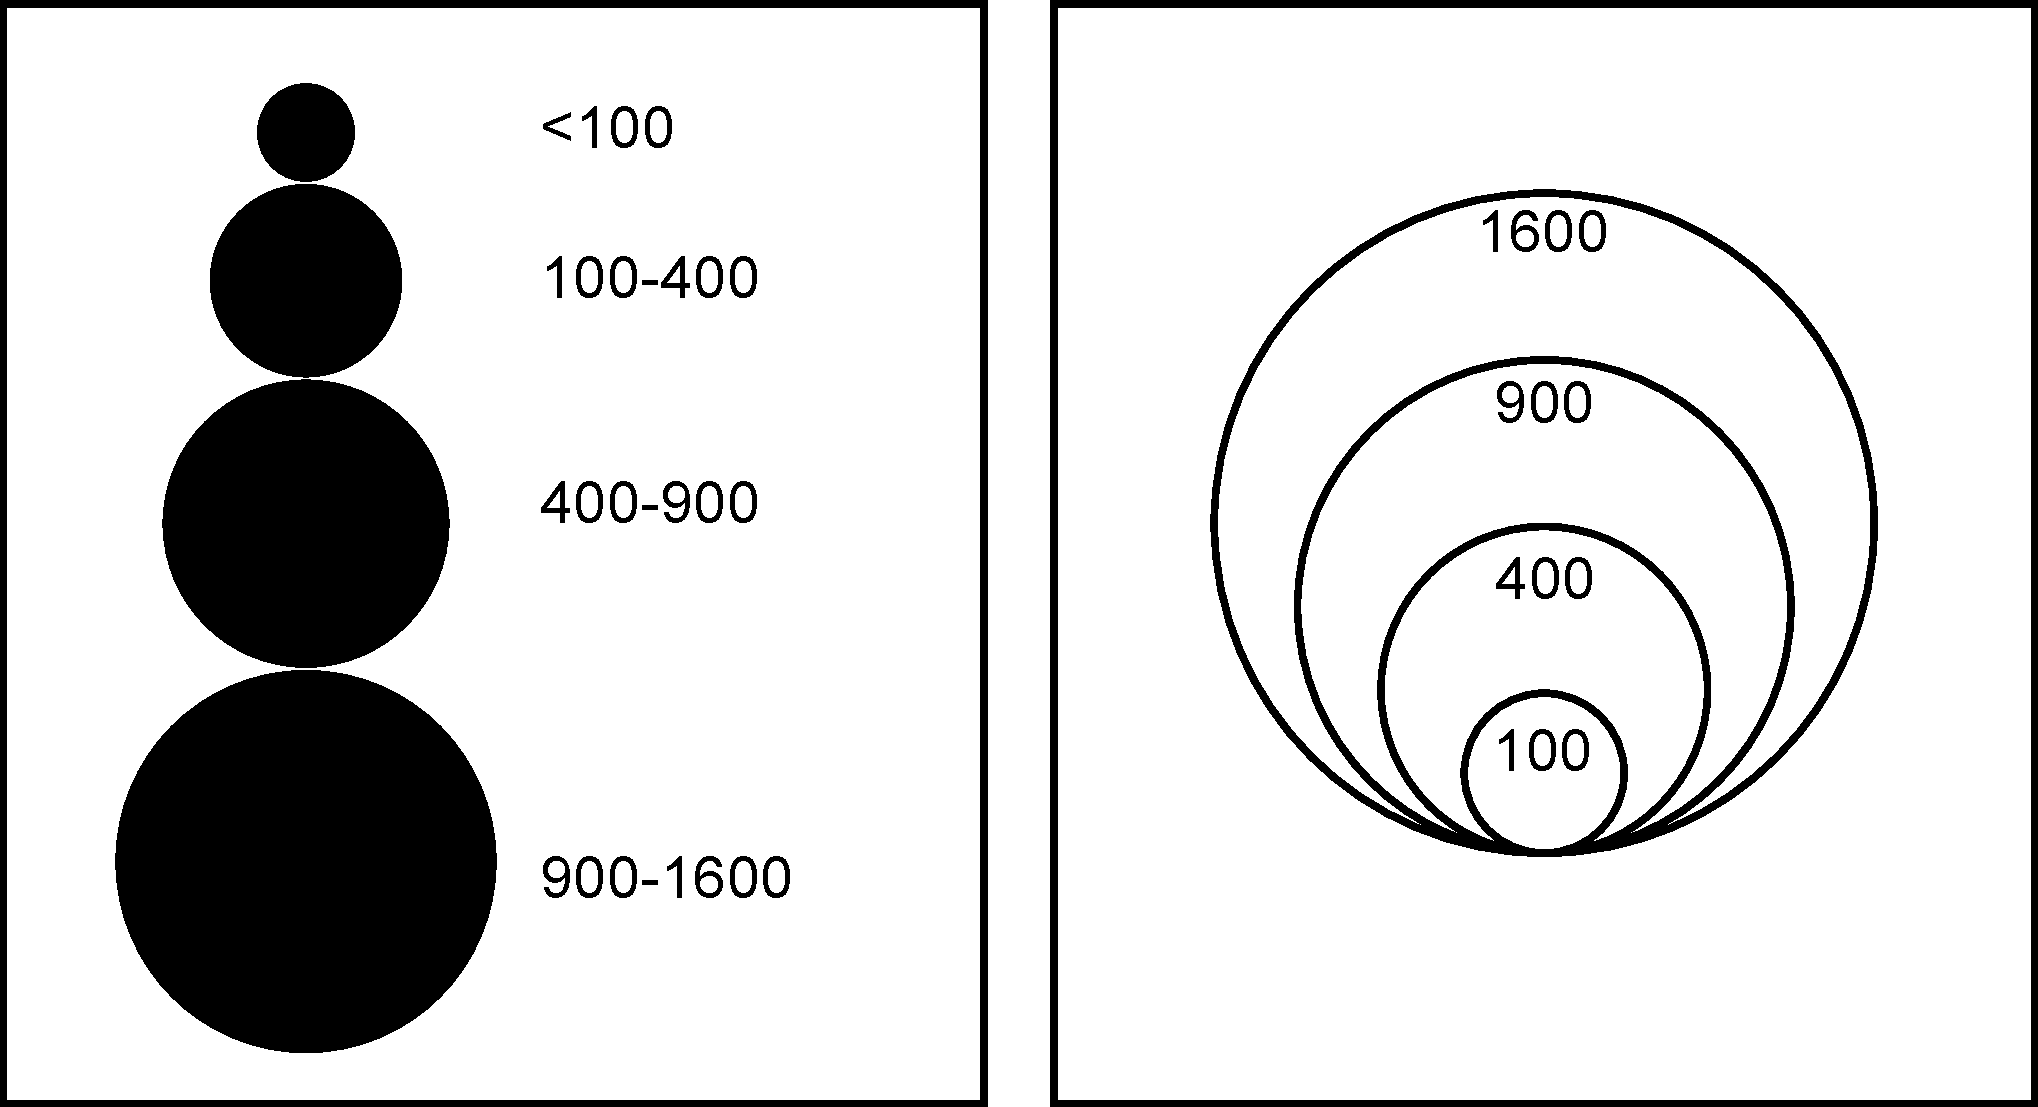
\includegraphics[width=.65\columnwidth]{Visualization/LegendProportionalSymbols.pdf}
\caption{\small Dos ejemplos de leyendas para un mapa de s�mbolos proporcionales.}
\label{Fig:LegendProportionalSymbols} 
\end{figure}


\subsection{Point density maps}

Point density maps are particularly suitable for countable variables such as population or crop yield. Thes quantities are represented using \textbf{repeated points}, whose number is proportional to the quantity itself. Each point represents a unitary value, and all the point within an area add up to the total value of the variable in it. All points have the same size and shape, unlike what we saw in the case of proportional symbols.

When creating a point density map, three parameters have to be define: the \textbf{value of each point} (that is, how many units of the variable the point represents), its \textbf{size} and its \textbf{position}.

The value of each point should be define \textbf{based on the range of values} covered by the variable, so points in the resulting map are not too scarce or too numerous. This value will be included in the legend, usually in text form, writing, for instance, that <<a point represents 1000 inhabitants>>.

Size must guarantee that points are visible and at the same time they do not take too much space in the map. The \textbf{optimal size is linked to the value of each point} that has been selected, and both parameters should be considered together, so as to find the best combination of them. 

The position of the points is of great importance, as it should not convey wrong information or cause the user to misinterpret its meaning. If we do not have any additional information, points should be regularly distributed, covering the whole area that correspond to the variable value. If, on the other hand, we have more information about the distribution of the variable, we should use it to give the points a more realistic position. For instance, if we are creating a density map with population values for regions, there should be more points in the surroundings of the cities within the region, since there are more inhabitants in those areas.

Another thing to consider is the meaning of the variable and whether or not the phenomenom that it represent can appear at a given point or not. For instance, if the variable that we are representing is the number of water bird know to nest in each region, it will be wrong to place the density points in forst areas or city ones, since it might be infered that birds are found there, which is not true.

Image \ref{Fig:MapPoints} shows an example of a point density map.


\begin{figure}[!hbt]
\centering
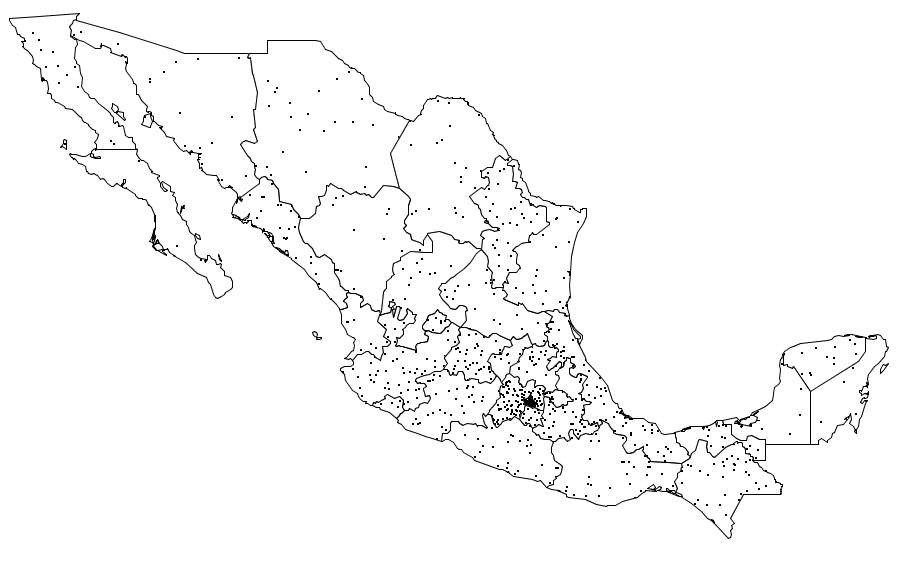
\includegraphics[width=.8\columnwidth]{Visualization/MapPoints.png}
\caption{\small Point density map.}
\label{Fig:MapPoints} 
\end{figure}


\subsection{Isoline map}

Isoline map are commonly used to represent \textbf{continuous variables}. Containing only lines, they mix well with other types of maps without being  obtrusive.

An isoline map is formed by a set of lines, each of them connecting points that have the same value of the variable being represented. These lines cannot cross with each other, since a point cannot have two valeus at the same time. The most common useage of isolines are contour lines in topographic maps, which represent points with the same elevation.

Isolines are defined by their \textbf{equidistance}, which defines the difference between the values represented by any two contiguous isolines. A lower equidistance means more isolines and a denser map.

Size is the only visual variable used with isolines. It is used to highlight those that representa a value that is multiple of a given number, to make the map easier to read. These lines are know as \textbf{index lines}.


\begin{figure}[!hbt]
\centering
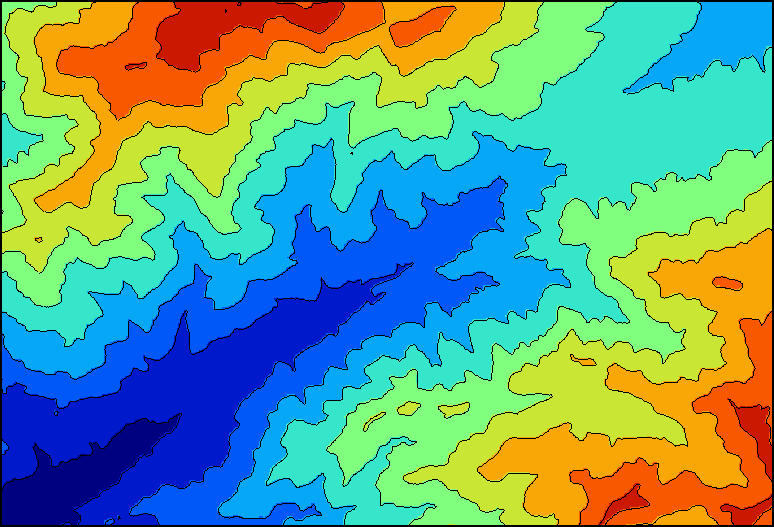
\includegraphics[width=.8\columnwidth]{Visualization/Isolineas.png}
\caption{\small Map with isolines and hypsometric tints.}
\label{Fig:Isolineas} 
\end{figure}


Lines are labeled with their value over the line itself, usually only on the index lines (the value of other lines between the index ones can be easily figured out knowing the equidistance).

A particular case of isolines are the so called \textbf{hypsometric tints}. apart from drawing the lines themselves, the areas between them are colored, each with a different color (usually using a graduated scheme).

Figure \ref{Fig:Isolines} shows an example of this.


\subsection{Choropleth maps}

Choropleth maps are a very common type of map in GIS. For instance, maps in figure \ref{Fig:IntervalClasses} were all choropleth maps.

In a choropleth map, there is a set of areas, each of them representing a single value of a variable. This value applies to the whole area, and is normally represented using hue applied to the areal symbol.

Choropleth maps have some  important limitations. One of them is the \textf{sharp change in the boundaries between area}. which might be interpreted as a abrupt change in the variable value in that boundary. This could hide the continuity of the variable distribution, in case it exists. Another problem is the \textbf{homogeneity within each area}, which might lead to thinking that the variable has a uniform distribution, even if that is false.


In many cases, an in order to correctly transmit the information contained in the variable, its values have to be \textbf{normalized using the area of each region}.


\section{Visualization in a GIS}

Now that we know the basic ideas about visualization and how thay are applied to maps, it is time to see how these are used in the context of a GIS. Two ideas are particularly relevant in this contexts: The fact that we work with \textbf{multiple layers} to be represented together, and the particularities of \textbf{on-screen rendering and the interactivity it offers}.

\subsection{Combining multiple layers}

In most cases, visualizing a layer alone by itself is not the best way of visualizing the information it contains. In a map, we normally find several types of information, and that is not just for the sake of space, but because it helps the map user to understand and interpret the main information. For instance, contour lines help to understand the meaning of a rivers and lakes, providing a valuable context.


When combining layers, we should try to create a sinergy between them, so they complement each other. This is mostly done by \textbf{correctly ordering the layers} and using \textbf{a symbology for each of them that does not interfere with the others}

When two layers have information for the same location, only the information of the layer on top will be seen. Layer ordering should maximize the information that is seen in the map, and prioritize the most important layers over those that contains secondary information.

We know that raster layers fill the space and contain values in all of their cells (pixels in the case of an image). For this reason, they will cover whatever is underneath and is not a good idea to place them at the top of the rendering order. Instead, they should be considered as \textbf{base layers on top of which the remaining layers are placed}.

With a similar reasoning, we can define the best way to order vector layers, placing polygon ones frist, then line ones, and then point ones at the top of the rendering order.


Sometimes, the rendering order \textbf{might be imposed by the meaning of layers}. For instance, if we are creating a map with a layer containing streams and another one containing roads, this last one should go on top of the first one, since roads usually pass over streams and not the other way round.

A common functionality that most GIS have is the use of \textbf{transparency} for layer. It can be applied to both raster and vector layers. Figure \ref{Fig:Transparency} was created using this technique. The polygon that defines the boundary of the watershed has a semi-transparent fill, which allows to see the shaded relief layer underneath. The result is a map in which the hydroogical meaning of the watershed is much clearer and easy to understand.

\begin{figure}[!hbt]
\centering
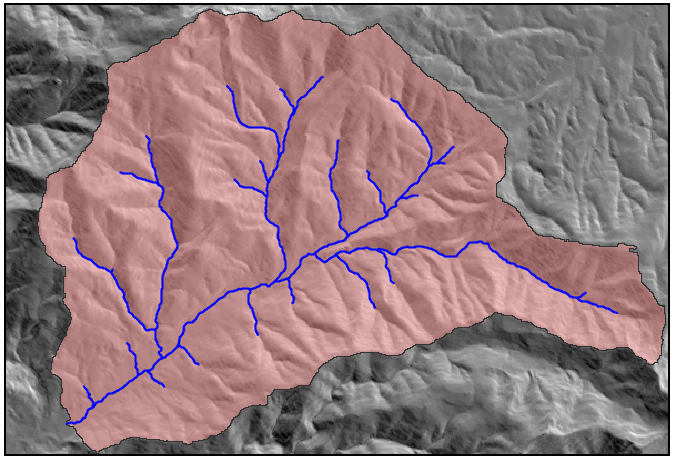
\includegraphics[width=.7\columnwidth]{Visualization/Transparency.png}
\caption{\small Combination of two layers using transparency.}
\label{Fig:Transparency} 
\end{figure}

In the case of raster layers, transparency can be applied partially, just rendering those cells that are within a given range of values.

If a variable is divided in many \textbf{separate layers} (horizontal division), the \texxtbf{same symbology} must be applied to all of them, in order to have a coherent map.


\subsection{Particularities of on-screen rendering}

Apart from the ideas that are aplied to printed maps, additional ones must be taken into account when the visualization takes place instead on a computer screen. A prineed map should not be designed in the same way as a map that is meant to be rendered on the screen.

The main elements to consider are the \textbf{low resolution of the screen} when compared to a printing device, and the \textbf{interactivity} of the visualization itself.

When creating a printed map, resolution is not a problem since the printing devices offer a level of detail that goes beyond what the cartographer might need. However, screen resolution is rather lower and certain elements might not be rendered with enough clarity. Although this elements can be used in printed maps, they should be replaced for on-screen maps. Among these problematic element we find \textbf{font with ornaments} such as shades, \textbf{fonts with serifs} (small lines attached to the end of the stroke to increase readability) or \textbf{texture fills of small size}.

Regarding interactivity, we must take into account that, unlike a printed map, an on-screen map is not a static element, but a dynamic one. That doesnt mean that the map changes by itself, but instead that the user can alter it using the tools that we have already seen (zoom, pan, etc.)

For instance, since the scale can be changed by the user, that might cause problem with certain elements such as symbols and text labels. If all elements are scaled proportionally, reducing the scale will make the labels too small and impossible to read. On the other hand, if the scale is increased, labels might be too large, as can be seen in figure \ref{Fig:ProblemsChangeScale}. 


\begin{figure}[!hbt]
\centering
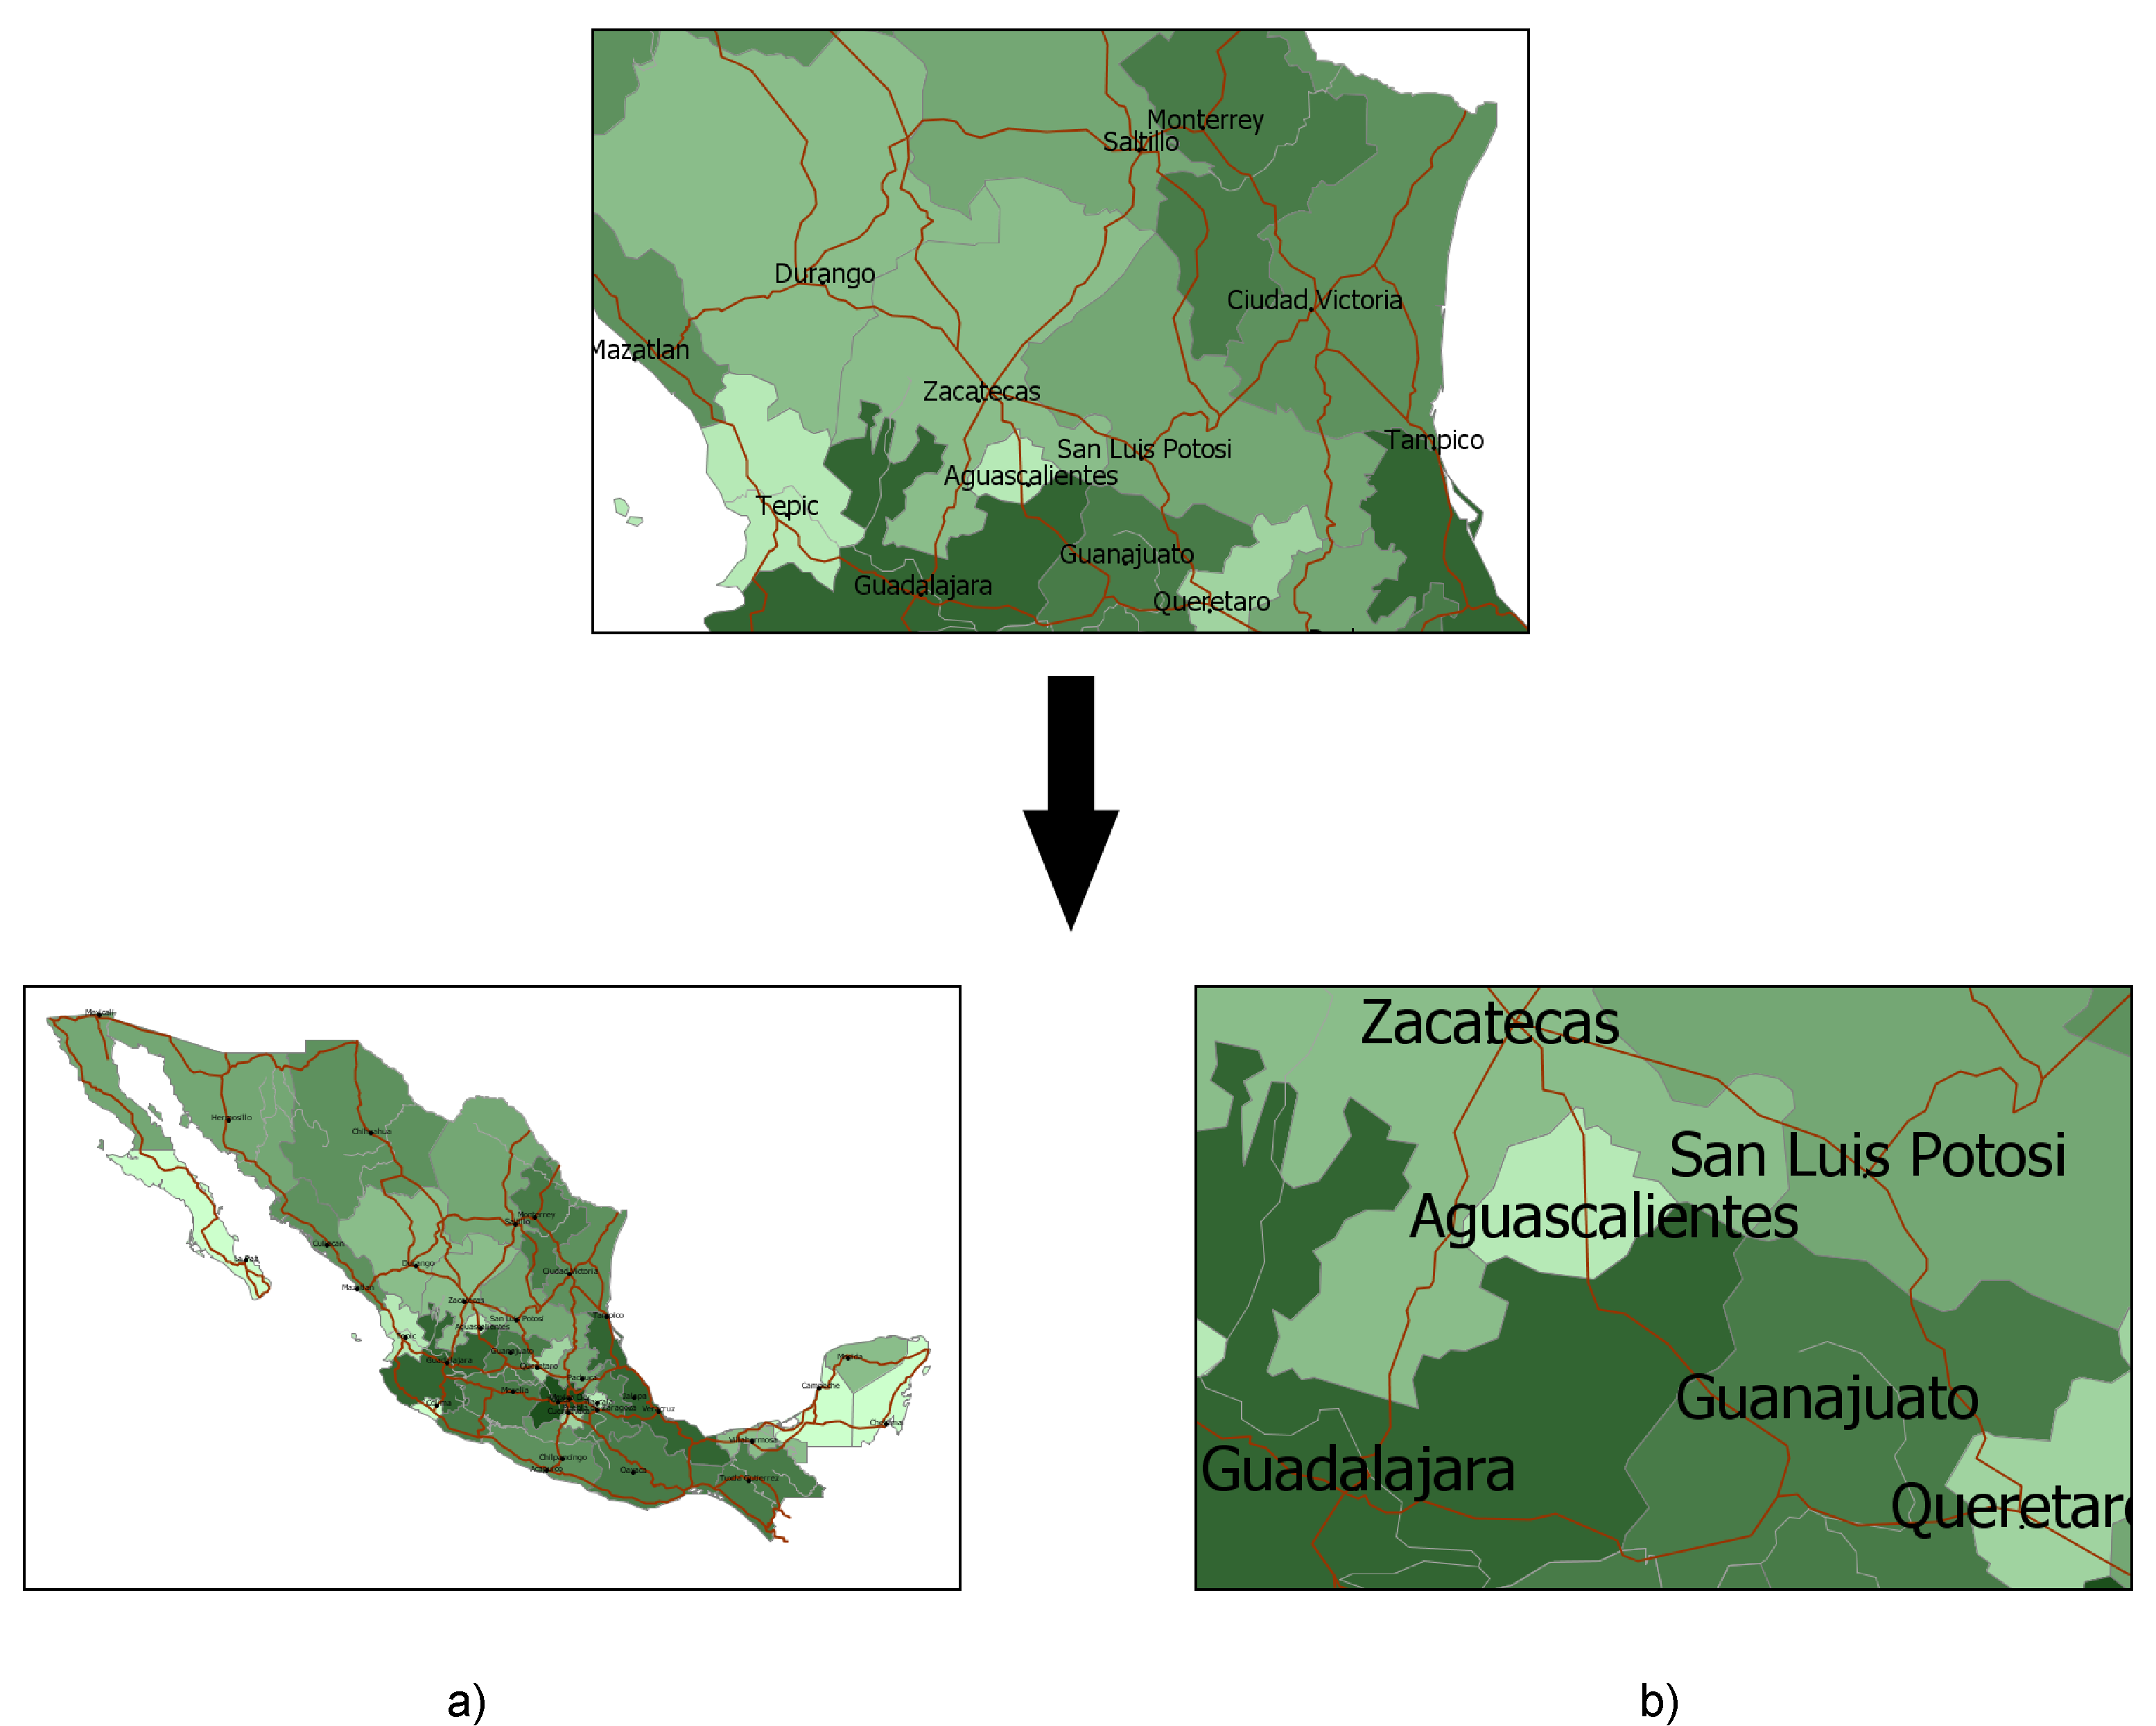
\includegraphics[width=\columnwidth]{Visualization/ProblemsChangeScale.pdf}
\caption{\small  A scale change modifes the size of symbols and text labels, and it can make them too small (a) or too large (b).}
\label{Fig:ProblemsChangeScale} 
\end{figure}

A solution to that is to use an \textbf{absolute size} for those elements, so they always have the same size regardless of the scale. With lower scales, however, that might result in maps that are saturated, as can be seen in figure \ref{Fig:SaturatedMap}.

\begin{figure}[!hbt]
\centering
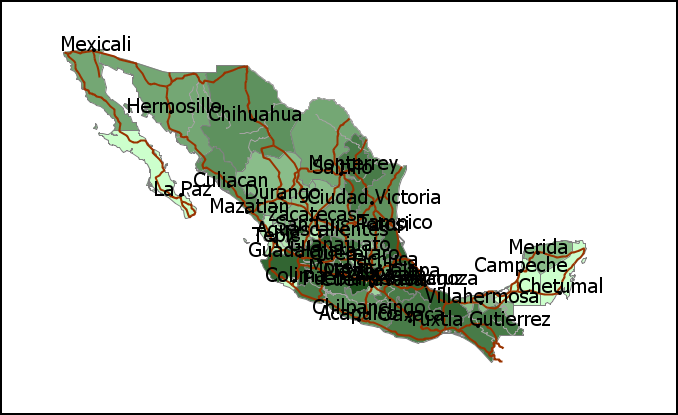
\includegraphics[width=.9\columnwidth]{Visualization/SaturatedMap.png}
\caption{\small Saturated map caused by rendering elements at a fixed size at a low scale.}
\label{Fig:SaturatedMap} 
\end{figure}

The ability of GIS to render layers at different scales can also cause \texbf{performance issues}. At low scales, the number of elements to be rendered can be too large, and painting them on the screen might take to omuch time. To avoid these problems, a \textbf{multiscalar approach} can be adopted, in which, depending on the scale, different layers and elements are rendered. For the same information, different versions with different levels of detail can be used, eachof them being used only at a given scale range.

\pagestyle{empty}
\tableofcontents
\end{mainmatter}

\cleardoublepage

\end{document}


